\documentclass[letterpaper,10pt]{book}
% Change to 10 pt
\usepackage{pdfpages}
\usepackage{morewrites}			% to counteract the no write space problem
\setcounter{tocdepth}{6}

\usepackage[framemethod=TikZ]{mdframed}

\usepackage{fancyhdr}

\usepackage{paralist}
\usepackage{amsmath}
\usepackage{amsfonts}
\usepackage{amssymb}
\usepackage{graphicx}

\usepackage{datetime}
%\usepackage{ulem}

%\usepackage[nottoc]{toobibind}

\usepackage[inline]{enumitem}

% Outer margin at 2.50 is exacty correct to fit the ``corruption alert'' tables
\usepackage[inner=1.0in, outer=2.50in, top=2.54cm,bottom=2.54cm, marginparwidth=2.25in]{geometry}

\usepackage{marginnote}
\usepackage{longtable}
\usepackage{booktabs}
\usepackage{xcolor}

\usepackage{soul}

%%%%%%%%%%%%
\definecolor{ForestGreen}{rgb}{0.00,0.29,0.098}
%%%%%%%%%%%%

\usepackage{marginnote}

\usepackage{imakeidx} 
\usepackage[
	backref=true,
	style=numeric,
%	citestyle=numeric,
	backend=bibtex
	]{biblatex}
\usepackage[driverfallback=hypertex,colorlinks=True]{hyperref}
\usepackage{cleveref}

\makeindex[name=scripture,columnsep=20pt, columnseprule=True,columns=3, title=Scripture References]
\makeindex[name=speaker,columnsep=20pt, columnseprule=True,,columns=2, title=Sermon Creator]
\makeindex[name=series,columnsep=20pt, columnseprule=True,,columns=2, title=Sermon Series]
\makeindex[name=date,columnsep=20pt, columnseprule=True,columns=2, title=Sermon Date]
\makeindex[name=event,columnsep=20pt, columnseprule=True,columns=2, title=Event]
\makeindex[name=topic,columnsep=20pt, columnseprule=True,columns=2, title=Topic]
\makeindex[name=AWIP,columnsep=20pt, columnseprule=True,columns=3, title=All Words in Passage]
\makeindex[name=NWIV,columnsep=20pt, columnseprule=True,columns=3, title=Number of Words in Verse]
\makeindex[name=PNIP,columnsep=20pt, columnseprule=True,columns=3, title=Proper Names in Passage]
\makeindex[name=PEIP,columnsep=20pt, columnseprule=True,columns=2, title=Prophetic Events in Passage]
\makeindex[name=TWPAQ,columnsep=20pt, columnseprule=True,columns=1, title=13-Word Phrases and Quotes]
\makeindex[name=PFTTIS,columnsep=20pt, columnseprule=False,columns=3, title=Phrases found 13 times in scripture]
\makeindex[name=WFTTIS,columnsep=20pt, columnseprule=False,columns=3, title=Words found 13 times in scripture]
\makeindex[name=WFITV,columnsep=20pt, columnseprule=False,columns=3, title=Words found in exactly 13 verses]
\makeindex[name=EVENTS,columnsep=20pt, columnseprule=False,columns=2, title=Sermon Log by Place]
\makeindex[name=QUESTIONS,columnsep=20pt, columnseprule=False,columns=2, title=Bible Questions]
\makeindex[name=DOCTRINES,columnsep=20pt, columnseprule=False,columns=2, title=Doctrines]
\makeindex[name=SONGS,columnsep=20pt, columnseprule=False,columns=1, title=Songs]
\makeindex[name=LOCATION,columnsep=20pt, columnseprule=False,columns= 2, title=Location]
\makeindex[name=FACEBOOK,columnsep=20pt, columnseprule=False,columns=2, title=Facebook]
\makeindex[name=DEVOTIONAL,columnsep=20pt, columnseprule=False,columns=2, title=Devotional Items]
%%%%%%%%%%%%%%%%% EXTRA COLORS
\definecolor{champagne}{rgb}{0.97,0.91,0.81}
\definecolor{bone}{rgb}{0.89,0.85,0.79}
\pagestyle{fancy}
\fancyhf{}
\fancyhead[LE,RO]{\today}
\fancyhead[RE,LO]{Daily Bible Reading}
\fancyhead[CE,CO]{-page \thepage  - }

\fancyfoot[CO,CE]{\leftmark}
%\fancyfoot[LE,RO]{CSCE 692, HW1}

\title{DBR\\
Daily \\ Reads}
\author{Keith Anthony \\
\today }
%+/ffffff +   \pagenumbering{gobble}
\bibliography{Bibliographies/All20220122}

\setlength{\fboxsep}{1.0pt}

\usepackage[utf8]{inputenc}
\usepackage{tikz}

\begin{document}
%%%%%%%%%%%% Tile Page

\begin{titlepage}

\begin{flushright}
\rightskip=-2.5cm
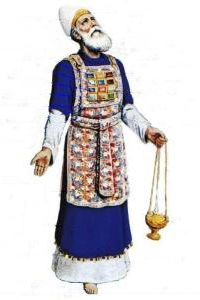
\includegraphics[width=50mm,scale=1.5]{Extras/Melchisedec.jpg}
\vspace{0.4in}  % Create a title for the document and write it in bold font
\LARGE{\textbf{\date}} % Again, do a line break
\linebreak 
% Create a subtitle \large{with Outlines, Statistics, Cross References, and Notes}
\vspace{0.5in}
\begin{flushleft}
\LARGE{Day \#65: Sunday, 6 March 2022 LITE  \\}\vspace{0.25in}
\LARGE{Joshua 1-3 Psalm 65 Proverb 6}
\end{flushleft}
\vspace{0.6in}
\bigskip

\normalsize{Xenia, Oh.\\}
\normalsize{created: \today}
\vspace{1.3in}

\end{flushright}
\end{titlepage}

\newpage 
\tableofcontents\hypertarget{TOC}{}
\listoffigures
\listoftables

\hyphenation{A-bim-e-lech bre-thren E-phra-im  Gib-e-o-nites Jer-u-sa-lem through-out Phil-i-stines The-o-phil-us Am-a-le-kites ven-geance Mesh-el-e-mi-ah onan-ism Phar-a-oh thoughts grev-ous-ness Hach-a-liah adul-ter-er Shad-rach}

%%%%%%%%%%%%%%%%% EXTRA COLORS
%%%%%%%%%%%%%%%%% EXTRA COLORS
%%%%%%%%%%%%%%%%% EXTRA COLORS
\definecolor{champagne}{rgb}{0.97,0.91,0.81}
\definecolor{bone}{rgb}{0.89,0.85,0.79}

\definecolor{ForestGreen}{rgb}{0.00,0.29,0.098}
\definecolor{GIVING}{cmyk}{1,0.0,0.72,.1}

\definecolor{MLPE}{cmyk}{1,1,0,.45}
\definecolor{SOCCER}{cmyk}{.77, 0, .42, .49}
\definecolor{PAYBILL}{cmyk}{0,0.83,0.76,0.07}
\definecolor{SERMON}{cmyk}{.14,.9,0,.30} % aka seance \href{http://www.flatuicolorpicker.com/purple-cmyk-color-model/}{seance}
\definecolor{BIBLE}{cmyk}{0,.17,.74,.17}
\definecolor{WORKBLUE}{cmyk}{1, .5, 0, .6}
\definecolor{myOrange}{cmyk}{0, .4, .98, .03}
\definecolor{myTan}{cmyk}{0.0,.07,.17,.10}
\definecolor{myRed}{cmyk}{0,1,1,0}
\definecolor{myWhite}{cmyk}{0,0,0,0}
\definecolor{BLUESoD}{cmyk}{.97,.84,0,.04}
\definecolor{WHITE}{cmyk}{0,0,0,0}
\definecolor{OLDGOLD}{cmyk}{0.05,0.3,1.00,0}
\definecolor{CASTLETON}{cmyk}{1,0,0.31,0.66}
\definecolor{cadmiumgreen}{rgb}{0.0, 0.42, 0.24}
\definecolor{jungle}{rgb}{0.203,0.4882,0.1718}
\definecolor{MYGOLD}{rgb}{1,.84,0}

\definecolor{MYLIGHTGRAY}{rgb}{.85,.85,.85}

\definecolor{codegreen}{rgb}{0,0.6,0}
\definecolor{codegray}{rgb}{0.5,0.5,0.5}
\definecolor{codepurple}{rgb}{0.58,0,0.82}
\definecolor{backcolour}{rgb}{0.95,0.95,0.92}


\mdfdefinestyle{MyFrame}{%
    linecolor=blue,
    outerlinewidth=2pt,
    roundcorner=5pt,
    innertopmargin=\baselineskip,
    innerbottommargin=\baselineskip,
    innerrightmargin=10pt,
    innerleftmargin=10pt,
    backgroundcolor=gray!25!white}


\mdfdefinestyle{MyFrame2}{%
    linecolor=black,
    outerlinewidth=2pt,
    roundcorner=5pt,
    innertopmargin=\baselineskip,
    innerbottommargin=\baselineskip,
    innerrightmargin=10pt,
    innerleftmargin=10pt,
    backgroundcolor=yellow!25!white}


%%%%%
%% for PFTTIS list
%%%%%

%%% And Joseph said unto
\index[PFTTIS]{And Joseph said unto!Genesis!Gen 40:008}
\index[PFTTIS]{And Joseph said unto!Genesis!Gen 40:012}
\index[PFTTIS]{And Joseph said unto!Genesis!Gen 41:025}
\index[PFTTIS]{And Joseph said unto!Genesis!Gen 42:014}
\index[PFTTIS]{And Joseph said unto!Genesis!Gen 42:018}
\index[PFTTIS]{And Joseph said unto!Genesis!Gen 44:015}
\index[PFTTIS]{And Joseph said unto!Genesis!Gen 45:003}
\index[PFTTIS]{And Joseph said unto!Genesis!Gen 45:004}
\index[PFTTIS]{And Joseph said unto!Genesis!Gen 46:031}
\index[PFTTIS]{And Joseph said unto!Genesis!Gen 48:009}
\index[PFTTIS]{And Joseph said unto!Genesis!Gen 48:018}
\index[PFTTIS]{And Joseph said unto!Genesis!Gen 50:019}
\index[PFTTIS]{And Joseph said unto!Genesis!Gen 50:024}


%%% a shadow
\index[PFTTIS]{a shadow!1Chronicles!1Chr 029:15}
\index[PFTTIS]{a shadow!Job!Job 008:09}
\index[PFTTIS]{a shadow!Job!Job 014:02}
\index[PFTTIS]{a shadow!Job!Job 017:07}
\index[PFTTIS]{a shadow!Psalm!Psa 102:011}
\index[PFTTIS]{a shadow!Psalm!Psa 144:004}
\index[PFTTIS]{a shadow!Ecclesiastes!Eccl 006:012}
\index[PFTTIS]{a shadow!Ecclesiastes!Eccl 008:013}
\index[PFTTIS]{a shadow!Isaiah!Isa 04:006}
\index[PFTTIS]{a shadow!Isaiah!Isa 25:004}
\index[PFTTIS]{a shadow!Jonah!Jnh 04:06}
\index[PFTTIS]{a shadow!Colossians!Col 02:017}
\index[PFTTIS]{a shadow!Hebews!Heb 10:001}

%%% blessed is the man
\index[PFTTIS]{blessed is the man!Psalm!Psa 001:001}
\index[PFTTIS]{blessed is the man!Psalm!Psa 032:002}
\index[PFTTIS]{blessed is the man!Psalm!Psa 034:008}
\index[PFTTIS]{blessed is the man!Psalm!Psa 065:004}
\index[PFTTIS]{blessed is the man!Psalm!Psa 084:005}
\index[PFTTIS]{blessed is the man!Psalm!Psa 084:012}
\index[PFTTIS]{blessed is the man!Psalm!Psa 094:012}
\index[PFTTIS]{blessed is the man!Psalm!Psa 112:001}
\index[PFTTIS]{blessed is the man!Proverbs!Pro 008:034}
\index[PFTTIS]{blessed is the man!Isaiah!Isa 056:002}
\index[PFTTIS]{blessed is the man!Jeremiah!Jer 017:007}
\index[PFTTIS]{blessed is the man!Romans!Rom 004:008}
\index[PFTTIS]{blessed is the man!James!Jam 001:012}


%%% carry them
\index[PFTTIS]{carry them!Leviticus!Lev 14:045}
\index[PFTTIS]{carry them!Numbers!Num 11:012}
\index[PFTTIS]{carry them!Joshua!Jsh 04:003}
\index[PFTTIS]{carry them!1Samuel!1Sam 20:040}
\index[PFTTIS]{carry them!1Kings!1Kng 08:046}
\index[PFTTIS]{carry them!2Chronicles!2Chr 06:036}
\index[PFTTIS]{carry them!Ezra!Ezra 05:015}
\index[PFTTIS]{carry them!Isaiah!Isa 40:011}
\index[PFTTIS]{carry them!Isaiah!Isa 41:016}
\index[PFTTIS]{carry them!Isaiah!Isa 57:013}
\index[PFTTIS]{carry them!Jeremiah!Jer 20:004}
\index[PFTTIS]{carry them!Jeremiah!Jer 20:005}
\index[PFTTIS]{carry them!Jeremiah!Jer 43:012}


\index[PFTTIS]{good tidings!2Samuel!2Sam 18:027}
\index[PFTTIS]{good tidings!1Kings!1Ki 01:042}
\index[PFTTIS]{good tidings!2Kings!2Ki 07:009 (2x)}
\index[PFTTIS]{good tidings!Isaiah!Isa 40:009 (2x)}
\index[PFTTIS]{good tidings!Isaiah!Isa 41:007}
\index[PFTTIS]{good tidings!Isaiah!Isa 52:007}
\index[PFTTIS]{good tidings!Isaiah!Isa 61:001}
\index[PFTTIS]{good tidings!Nahum!Nah 01:005}
\index[PFTTIS]{good tidings!Luke!Lk 02:010}
\index[PFTTIS]{good tidings!1Thessalonians!1Thess 03:006}


%%% dead body
\index[PFTTIS]{dead body!Leviticus!Lev 21:011}
\index[PFTTIS]{dead body!Numbers!Num 06:006}
\index[PFTTIS]{dead body!Numbers!Num 09:006}
\index[PFTTIS]{dead body!Numbers!Num 09:007}
\index[PFTTIS]{dead body!Numbers!Num 09:010}
\index[PFTTIS]{dead body!Numbers!Num 09:011}
\index[PFTTIS]{dead body!Numbers!Num 09:013}
\index[PFTTIS]{dead body!Numbers!Num 09:016}
\index[PFTTIS]{dead body!2Kings!2Ki 08:005}
\index[PFTTIS]{dead body!Isaiah!Isa 26:019}
\index[PFTTIS]{dead body!Jeremiah!Jer 26:023}
\index[PFTTIS]{dead body!Jeremiah!Jer 36:030}
\index[PFTTIS]{dead body!Haggai!Hag 02:013}

%%% great sea
\index[PFTTIS]{great sea!Numbers!Num 34:006}
\index[PFTTIS]{great sea!Numbers!Num 34:007}
\index[PFTTIS]{great sea!Joshua!Jos 01:004}
\index[PFTTIS]{great sea!Joshua!Jos 09:001}
\index[PFTTIS]{great sea!Joshua!Jos 15:012}
\index[PFTTIS]{great sea!Joshua!Jos 15:047}
\index[PFTTIS]{great sea!Joshua!Jos 23:004}
\index[PFTTIS]{great sea!Ezekiel!Eze 47:010}
\index[PFTTIS]{great sea!Ezekiel!Eze 47:015}
\index[PFTTIS]{great sea!Ezekiel!Eze 47:019}
\index[PFTTIS]{great sea!Ezekiel!Eze 47:020}
\index[PFTTIS]{great sea!Ezekiel!Eze 48:028}
\index[PFTTIS]{great sea!Daniel!Dan 07:002}


%%% have forsaken me
\index[PFTTIS]{have forsaken me!Judges!Jdg 10:013}
\index[PFTTIS]{have forsaken me!1Samuel!1Sam 08:008}
\index[PFTTIS]{have forsaken me!1Kings!1Ki 11:033}
\index[PFTTIS]{have forsaken me!2Kings!2Ki 22:017}
\index[PFTTIS]{have forsaken me!2Chronicles!2Chr 12:005}
\index[PFTTIS]{have forsaken me!2Chronicles!2Chr 34:025}
\index[PFTTIS]{have forsaken me!Jeremiah!Jer 01:016}
\index[PFTTIS]{have forsaken me!Jeremiah!Jer 02:013}
\index[PFTTIS]{have forsaken me!Jeremiah!Jer 05:007}
\index[PFTTIS]{have forsaken me!Jeremiah!Jer 05:019}
\index[PFTTIS]{have forsaken me!Jeremiah!Jer 16:011 (2x)}
\index[PFTTIS]{have forsaken me!Jeremiah!Jer 19:004}

%%% no king
\index[PFTTIS]{no king!Judges!Jdg 17:06}
\index[PFTTIS]{no king!Judges!Jdg 18:01}
\index[PFTTIS]{no king!Judges!Jdg 19:01}
\index[PFTTIS]{no king!Judges!Jdg 21:25}
\index[PFTTIS]{no king!1Kings!1Ki 22:47}
\index[PFTTIS]{no king!2Kings!2Ki 23:25}
\index[PFTTIS]{no king!Nehemiah!Neh 13:26}
\index[PFTTIS]{no king!Psalms!Psa 033:016}
\index[PFTTIS]{no king!Proverbs!Pro 30:27}
\index[PFTTIS]{no king!Daniel!Dan 02:10}
\index[PFTTIS]{no king!Hosea!Hos 10:03}
\index[PFTTIS]{no king!Micah!Mic 04:09}
\index[PFTTIS]{no king!John!Jhn 19:15}


%%% rebellious house
\index[PFTTIS]{rebellious house!Exodus!Exo 02:005}
\index[PFTTIS]{rebellious house!Exodus!Exo 02:006}
\index[PFTTIS]{rebellious house!Exodus!Exo 02:008}
\index[PFTTIS]{rebellious house!Exodus!Exo 03:009}
\index[PFTTIS]{rebellious house!Exodus!Exo 03:026}
\index[PFTTIS]{rebellious house!Exodus!Exo 03:027}
\index[PFTTIS]{rebellious house!Exodus!Exo 12:002 (2x)}
\index[PFTTIS]{rebellious house!Exodus!Exo 12:003}
\index[PFTTIS]{rebellious house!Exodus!Exo 12:009}
\index[PFTTIS]{rebellious house!Exodus!Exo 12:025}
\index[PFTTIS]{rebellious house!Exodus!Exo 17:012}
\index[PFTTIS]{rebellious house!Exodus!Exo 24:003}

%%% seek him
\index[PFTTIS]{seek him!Deuteronomy!Deu 04:029}\index[PFTTIS]{seek him!1Samuel!1Sam 23:025}
\index[PFTTIS]{seek him!1Chronicles!1Chr 28:009}
\index[PFTTIS]{seek him!2Chronicles!1Chr 15:002}
\index[PFTTIS]{seek him!Ezra!Ezr 08:022}
\index[PFTTIS]{seek him!Psalms!Psa 022:026}
\index[PFTTIS]{seek him!Psalms!Psa 024:006}
\index[PFTTIS]{seek him!Psalms!Psa 119:002}
\index[PFTTIS]{seek him!SoS!SoS 03:002}
\index[PFTTIS]{seek him!SoS!SoS 06:001}
\index[PFTTIS]{seek him!Hosea!Hos 07:010}
\index[PFTTIS]{seek him!Amos!Amo 05:008}
\index[PFTTIS]{seek him!Hebrews!Heb 11:0063}


%%% seek ye
\index[PFTTIS]{seek ye!Isaiah!Isa 34:016}
\index[PFTTIS]{seek ye!Isaiah!Isa 45:019}
\index[PFTTIS]{seek ye!Isaiah!Isa 55:006}
\index[PFTTIS]{seek ye!Amos!Amos 5:004}
\index[PFTTIS]{seek ye!John!John 1:38}
\index[PFTTIS]{seek ye!John!John 18:4}
\index[PFTTIS]{seek ye!John!John 18:7}
\index[PFTTIS]{seek ye!Matthew!Matt 6:33}
\index[PFTTIS]{seek ye!Numbers!Num 16:10}
\index[PFTTIS]{seek ye!Luke!Luke 12:31}
\index[PFTTIS]{seek ye!Luke!Luke 24:5}
\index[PFTTIS]{seek ye!Psalm!Psa 27:8}
\index[PFTTIS]{seek ye!Zephaniah!Zeph 2:3}

%%% the uncircumcised
\index[PFTTIS]{the uncircumcised!Genesis!Gen 17:014}
\index[PFTTIS]{the uncircumcised!Judges!Jdg 14:003}
\index[PFTTIS]{the uncircumcised!Judges!Jdg 15:018}
\index[PFTTIS]{the uncircumcised!2Samuel!2Sam 01:020}
\index[PFTTIS]{the uncircumcised!Isaiah!Isa 02:001}
\index[PFTTIS]{the uncircumcised!Jeremiah!Jer 09:025}
\index[PFTTIS]{the uncircumcised!Ezekiel!Eze 28:010}
\index[PFTTIS]{the uncircumcised!Ezekiel!Eze 31:018}
\index[PFTTIS]{the uncircumcised!Ezekiel!Eze 32:019}
\index[PFTTIS]{the uncircumcised!Ezekiel!Eze 32:027}
\index[PFTTIS]{the uncircumcised!Ezekiel!Eze 32:028}
\index[PFTTIS]{the uncircumcised!Ezekiel!Eze 32:029}
\index[PFTTIS]{the uncircumcised!Ezekiel!Eze 32:032}

%%% worship him
\index[PFTTIS]{worship him!Psalms!Psa 97:007}
\index[PFTTIS]{worship him!Zephaniah!Zeph 02:011}
\index[PFTTIS]{worship him!Matthew!Matt 02:002}
\index[PFTTIS]{worship him!Matthew!Matt 02:008}
\index[PFTTIS]{worship him!John!John 04:023}
\index[PFTTIS]{worship him!John!John 04:024 (2x)} 
\index[PFTTIS]{worship him!Acts!Acts 17:023}
\index[PFTTIS]{worship him!Hebrews!Heb 01:006}
\index[PFTTIS]{worship him!Revelation!Rev 04:010}
\index[PFTTIS]{worship him!Revelation!Rev 13:008}
\index[PFTTIS]{worship him!Revelation!Rev 14:007}
\index[PFTTIS]{worship him!Revelation!Rev 19:010}


%%%%%
%% for PFTTIS list
%%%%%

%%% afflictions
\index[WFTTIS]{afflictions!Psalms!Psa 34:019}
\index[WFTTIS]{afflictions!Psalms!Psa 132:001}
\index[WFTTIS]{afflictions!Acts!Acts 07:010}
\index[WFTTIS]{afflictions!Acts!Acts 20:023}
\index[WFTTIS]{afflictions!2Corinthians!2Cor 06:004}
\index[WFTTIS]{afflictions!Colossians!Col 01:024}
\index[WFTTIS]{afflictions!1Thessalonians!1Thess 03:003}
\index[WFTTIS]{afflictions!2Timothy!2Tim 01:008}
\index[WFTTIS]{afflictions!2Timothy!2Tim 03:011}
\index[WFTTIS]{afflictions!2Timothy!2Tim 04:005}
\index[WFTTIS]{afflictions!Hebrews!Heb 10:032}
\index[WFTTIS]{afflictions!Hebrews!Heb 10:033}
\index[WFTTIS]{afflictions!1Peter!1Pet 05:009}

%%% acsend
\index[WFTTIS]{acsend!Joshua!Jos 06:05}
\index[WFTTIS]{acsend!Psalm!Psa 024:003}
\index[WFTTIS]{acsend!Psalm!Psa 135:007}
\index[WFTTIS]{acsend!Psalm!Psa 139:008}
\index[WFTTIS]{acsend!Isaiah!Isa 14:013}
\index[WFTTIS]{acsend!Isaiah!Isa 14:014}
\index[WFTTIS]{acsend!Jeremiah!Jer 10:013}
\index[WFTTIS]{acsend!Jeremiah!Jer 51:016}
\index[WFTTIS]{acsend!Ezekiel!Eze 38:009}
\index[WFTTIS]{acsend!John!John 06:062}
\index[WFTTIS]{acsend!John!John 20:017}
\index[WFTTIS]{acsend!Romans!Rom 10:006}
\index[WFTTIS]{acsend!Revelation!Rev 17:008}

%%% Assyrian
\index[WFTTIS]{Assyrian!Isaiah!Isa 10:005}
\index[WFTTIS]{Assyrian!Isaiah!Isa 10:024}
\index[WFTTIS]{Assyrian!Isaiah!Isa 14:025}
\index[WFTTIS]{Assyrian!Isaiah!Isa 19:023}
\index[WFTTIS]{Assyrian!Isaiah!Isa 23:013}
\index[WFTTIS]{Assyrian!Isaiah!Isa 30:031}
\index[WFTTIS]{Assyrian!Isaiah!Isa 31:008}
\index[WFTTIS]{Assyrian!Isaiah!Isa 52:004}
\index[WFTTIS]{Assyrian!Ezekiel!Eze 31:003}
\index[WFTTIS]{Assyrian!Hosea!Hos 05:013}
\index[WFTTIS]{Assyrian!Hosea!Hos 11:005}
\index[WFTTIS]{Assyrian!Micah!Hos 05:005}
\index[WFTTIS]{Assyrian!Micah!Hos 05:006}

%%% blot
\index[WFTTIS]{blot!Exodus!Exo 32:032}
\index[WFTTIS]{blot!Exodus!Exo 32:033}
\index[WFTTIS]{blot!Numbers!Num 05:026}
\index[WFTTIS]{blot!Deuteronomy!Deut 09:014}
\index[WFTTIS]{blot!Deuteronomy!Deut 25:019}
\index[WFTTIS]{blot!Deuteronomy!Deut 29:020}
\index[WFTTIS]{blot!2Kings!2Ki 14:027}
\index[WFTTIS]{blot!Job!Job 31:007}
\index[WFTTIS]{blot!Psalms!Psa 51:001}
\index[WFTTIS]{blot!Psalms!Psa 51:009}
\index[WFTTIS]{blot!Proverbs!Pro 09:007}
\index[WFTTIS]{blot!Jeremiah!Jer 18:023}
\index[WFTTIS]{blot!Revelation!Rev 03:005}


%%% chain
\index[WFTTIS]{chain!Genesis!Gen 41:042}
\index[WFTTIS]{chain!1Kings!1Ki 07:017}
\index[WFTTIS]{chain!Psalms!Psa 73:006}
\index[WFTTIS]{chain!SoS!Sos 04:009}
\index[WFTTIS]{chain!Lamentations!Lam 03:007}
\index[WFTTIS]{chain!Ezekiel!Eze 07:023}
\index[WFTTIS]{chain!Ezekiel!Eze 16:011}
\index[WFTTIS]{chain!Daniel!Dan 05:007}
\index[WFTTIS]{chain!Daniel!Dan 05:016}
\index[WFTTIS]{chain!Daniel!Dan 05:029}
\index[WFTTIS]{chain!Acts!Acts 28:020}
\index[WFTTIS]{chain!2Timothy!2Tim 01:016}
\index[WFTTIS]{chain!Revelation!Rev 20:001}


%%% controversy
\index[WFTTIS]{controversy!Deuteronomy!Deu 17:008}
\index[WFTTIS]{controversy!Deuteronomy!Deu 19:017}
\index[WFTTIS]{controversy!Deuteronomy!Deu 21:005}
\index[WFTTIS]{controversy!Deuteronomy!Deu 25:001}
\index[WFTTIS]{controversy!2Samuel!2Sam 15:002}
\index[WFTTIS]{controversy!Isaiah!Isa 34:008}
\index[WFTTIS]{controversy!Jeremiah!Jer 25:031}
\index[WFTTIS]{controversy!Ezekiel!Eze 44:024}
\index[WFTTIS]{controversy!Hosea!Hos 04:001}
\index[WFTTIS]{controversy!Hosea!Hos 12:002}
\index[WFTTIS]{controversy!Micah!Mic 06:002 (2x)}
\index[WFTTIS]{controversy!1Timothy!1Tim 03:016}


%%% Dagon/Dagon's
\index[WFTTIS]{Dagon!Judges!Jdg 16:023}
\index[WFTTIS]{Dagon!1Samuel!1Sam 05:002 (2x)}
\index[WFTTIS]{Dagon!1Samuel!1Sam 05:003 (2x)}
\index[WFTTIS]{Dagon!1Samuel!1Sam 05:004 (3x)}
\index[WFTTIS]{Dagon!1Samuel!1Sam 05:005 (3x)}
\index[WFTTIS]{Dagon!1Samuel!1Sam 05:007}
\index[WFTTIS]{Dagon!1Chronicles!1Chr 10:010}

%%% disobedient
\index[WFTTIS]{disobedient!1Kings!1Ki 13:026}
\index[WFTTIS]{disobedient!Nehemiah!Neh 09:026}
\index[WFTTIS]{disobedient!Luke!Luke 01:017}
\index[WFTTIS]{disobedient!Acts!Acts 26:019}
\index[WFTTIS]{disobedient!Romans!Rom 01:030}
\index[WFTTIS]{disobedient!Romans!Rom 10:021}
\index[WFTTIS]{disobedient!1Timothy!1Tim 01:009}
\index[WFTTIS]{disobedient!2Timothy!2Tim 03:002}
\index[WFTTIS]{disobedient!Titus!Titus 01:016}
\index[WFTTIS]{disobedient!Titus!Titus 03:003}
\index[WFTTIS]{disobedient!1Peter!1Pet 02:007}
\index[WFTTIS]{disobedient!1Peter!1Pet 02:008}
\index[WFTTIS]{disobedient!1Peter!1Pet 03:020}


%%% doubt
\index[WFTTIS]{doubt!Genesis!Gen 37:033}
\index[WFTTIS]{doubt!Deuteronomy!Deu 28:066}
\index[WFTTIS]{doubt!Job!Job 12:002}
\index[WFTTIS]{doubt!Matthew!Matt 14:031}
\index[WFTTIS]{doubt!Matthew!Matt 21:021}
\index[WFTTIS]{doubt!Mark!Mk 11:023}
\index[WFTTIS]{doubt!Luke!Lk 11:020}
\index[WFTTIS]{doubt!John!Jhn 10:024}
\index[WFTTIS]{doubt!Acts!Acts 02:012}
\index[WFTTIS]{doubt!Acts!Acts 28:004}
\index[WFTTIS]{doubt!1Corinthians!1Cor 09:010}
\index[WFTTIS]{doubt!Galatians!Gal 04:020}
\index[WFTTIS]{doubt!1John!1Jhn 02:019}


%%% dungeon
\index[WFTTIS]{dungeon!Genesis!Gen 40:015}
\index[WFTTIS]{dungeon!Genesis!Gen 41:014}
\index[WFTTIS]{dungeon!Exodus!Exo 12:029}
\index[WFTTIS]{dungeon!Jeremiah!Jer 37:016}
\index[WFTTIS]{dungeon!Jeremiah!Jer 38:006 (2x)}
\index[WFTTIS]{dungeon!Jeremiah!Jer 38:007}
\index[WFTTIS]{dungeon!Jeremiah!Jer 38:009}
\index[WFTTIS]{dungeon!Jeremiah!Jer 38:010}
\index[WFTTIS]{dungeon!Jeremiah!Jer 38:011}
\index[WFTTIS]{dungeon!Jeremiah!Jer 38:013}
\index[WFTTIS]{dungeon!Lamentations!Lam 03:053}
\index[WFTTIS]{dungeon!Lamentations!Lam 03:055}


%%% error
\index[WFTTIS]{error!2Samuel!2Sam 06:007}
\index[WFTTIS]{error!Job!Job 19:004}
\index[WFTTIS]{error!Ecclesiastes!Ecc 05:006}
\index[WFTTIS]{error!Ecclesiastes!Ecc 10:005}
\index[WFTTIS]{error!Isaiah!Isa 32:006}
\index[WFTTIS]{error!Daniel!Dan 06:004}
\index[WFTTIS]{error!Matthew!Matt 27:064}
\index[WFTTIS]{error!Romans!Rom 01:027}
\index[WFTTIS]{error!James!Jam 05:020}
\index[WFTTIS]{error!2Peter!2Pet 02:018}
\index[WFTTIS]{error!2Peter!2Pet 03:017}
\index[WFTTIS]{error!1John!1Jn 04:006}
\index[WFTTIS]{error!Jude!Jude 01:011}

%%% fourish
\index[WFTTIS]{fourish!Psalms!Psa 072:007}
\index[WFTTIS]{fourish!Psalms!Psa 072:016}
\index[WFTTIS]{fourish!Psalms!Psa 092:007}
\index[WFTTIS]{fourish!Psalms!Psa 092:012}
\index[WFTTIS]{fourish!Psalms!Psa 092:013}
\index[WFTTIS]{fourish!Psalms!Psa 132:018}
\index[WFTTIS]{fourish!Proverbs!Pro 11:28}
\index[WFTTIS]{fourish!Proverbs!Pro 14:11}
\index[WFTTIS]{fourish!Ecclesiastes!Ecc 12:05}
\index[WFTTIS]{fourish!SongOfSolomon!SOS 07:12}
\index[WFTTIS]{fourish!Isaiah!Isa 17:11}
\index[WFTTIS]{fourish!Isaiah!Isa 66:14}
\index[WFTTIS]{fourish!Ezekiel!Eze 17:24}




%%% giants
\index[WFTTIS]{giants!Genesis!Gen 06:004}
\index[WFTTIS]{giants!Numbers!Num 13:033}
\index[WFTTIS]{giants!Deuteronomy!Deut 02:011}
\index[WFTTIS]{giants!Deuteronomy!Deut 02:021}
\index[WFTTIS]{giants!Deuteronomy!Deut 03:011}
\index[WFTTIS]{giants!Deuteronomy!Deut 03:013}
\index[WFTTIS]{giants!Joshua!Josh 12:004}
\index[WFTTIS]{giants!Joshua!Josh 13:012}
\index[WFTTIS]{giants!Joshua!Josh 15:008}
\index[WFTTIS]{giants!Joshua!Josh 17:015}
\index[WFTTIS]{giants!Joshua!Josh 16:016}

%%% good man
\index[WFTTIS]{good man!2 Samuel!2Sa 18:27}
%(1) Psalms 37:23 [5]
%(1) Psalms 112:5 [2]
%(1) Proverbs 12:2 [2]
%(1) Proverbs 13:22 [2]
%(1) Proverbs 14:14 [14]
%(1) Micah 7:2 [2]
%(1) Matthew 12:35 [2]
%(1) Luke 6:45 [2]
%(1) Luke 23:50 [15]
%(1) John 7:12 [17]
%(1) Acts 11:24 [5]
%(1) Romans 5:7 [14]

%%% Hinnom
\index[WFTTIS]{Hinnom!Joshua!Jsh 15:008}
\index[WFTTIS]{Hinnom!Joshua!Jsh 18:016}
\index[WFTTIS]{Hinnom!2Kings!2Ki 23:010}
\index[WFTTIS]{Hinnom!2Chronicles!2Chr 28:003}
\index[WFTTIS]{Hinnom!2Chronicles!2Chr 33:006}
\index[WFTTIS]{Hinnom!Nehemiah!Neh 11:030}
\index[WFTTIS]{Hinnom!Jeremiah!Jer 07:031}
\index[WFTTIS]{Hinnom!Jeremiah!Jer 07:032}
\index[WFTTIS]{Hinnom!Jeremiah!Jer 19:002}
\index[WFTTIS]{Hinnom!Jeremiah!Jer 19:006}
\index[WFTTIS]{Hinnom!Jeremiah!Jer 32:035}

%%% inclined
\index[WFTTIS]{inclined!Judges!Jdg 09:003}
\index[WFTTIS]{inclined!Psalms!Psa 040:001}
\index[WFTTIS]{inclined!Psalms!Psa 116:002}
\index[WFTTIS]{inclined!Psalms!Psa 119:112}
\index[WFTTIS]{inclined!Proverbs!Pro 05:13}
\index[WFTTIS]{inclined!Jeremiah!Jer 07:24}
\index[WFTTIS]{inclined!Jeremiah!Jer 07:26}
\index[WFTTIS]{inclined!Jeremiah!Jer 11:08}
\index[WFTTIS]{inclined!Jeremiah!Jer 17:23}
\index[WFTTIS]{inclined!Jeremiah!Jer 25:04}
\index[WFTTIS]{inclined!Jeremiah!Jer 34:14}
\index[WFTTIS]{inclined!Jeremiah!Jer 35:15}
\index[WFTTIS]{inclined!Jeremiah!Jer 44:05}


%%% laughed
\index[WFTTIS]{laughed!Genesis!Gen 17:017}
\index[WFTTIS]{laughed!Genesis!Gen 18:012}
\index[WFTTIS]{laughed!Genesis!Gen 18:015}
\index[WFTTIS]{laughed!2Kings!2Ki 19:021}
\index[WFTTIS]{laughed!2Chronicles!2Chr 30:010}
\index[WFTTIS]{laughed!Nehemiah!Neh 02:019}
\index[WFTTIS]{laughed!Job!Job 12:004}
\index[WFTTIS]{laughed!Job!Job 29:024}
\index[WFTTIS]{laughed!Isaiah!Isa 37:022}
\index[WFTTIS]{laughed!Ezekiel!Ezek 23:032}
\index[WFTTIS]{laughed!Matthew!Matt 09:024}
\index[WFTTIS]{laughed!Mark!Mk 05:040}
\index[WFTTIS]{laughed!Luke!Lk 08:053}

%%% liar
\index[WFTTIS]{liar!Job!Job 24:025}
\index[WFTTIS]{liar!Proverbs!Pro 17:004}
\index[WFTTIS]{liar!Proverbs!Pro 19:022}
\index[WFTTIS]{liar!Proverbs!Pro 30:006}
\index[WFTTIS]{liar!Jeremiah!Jer 15:018}
\index[WFTTIS]{liar!John!Jhn 08:044}
\index[WFTTIS]{liar!John!Jhn 08:055}
\index[WFTTIS]{liar!Romans!Rom 03:004}
\index[WFTTIS]{liar!1John!1Jhn 01:010}
\index[WFTTIS]{liar!1John!1Jhn 02:004}
\index[WFTTIS]{liar!1John!1Jhn 02:022}
\index[WFTTIS]{liar!1John!1Jhn 04:020}
\index[WFTTIS]{liar!1John!1Jhn 05:010}

%%% palsy
\index[WFTTIS]{palsy!Matthew!Matt 04:024}
\index[WFTTIS]{palsy!Matthew!Matt 08:006}
\index[WFTTIS]{palsy!Matthew!Matt 09:002}
\index[WFTTIS]{palsy!Matthew!Matt 09:006}
\index[WFTTIS]{palsy!Mark!Mk 02:003}
\index[WFTTIS]{palsy!Mark!Mk 02:004}
\index[WFTTIS]{palsy!Mark!Mk 02:005}
\index[WFTTIS]{palsy!Mark!Mk 02:009}
\index[WFTTIS]{palsy!Mark!Mk 02:010}
\index[WFTTIS]{palsy!Luke!Lk 05:018}
\index[WFTTIS]{palsy!Luke!Lk 05:024}
\index[WFTTIS]{palsy!Acts!Acts 09:033}

%%% Profitable
\index[WFTTIS]{profitable!Job!Job 22:002 (2x)}
\index[WFTTIS]{profitable!Ecclesiastes!Ecc 10:010}
\index[WFTTIS]{profitable!Isaiah!Isa 44:010}
\index[WFTTIS]{profitable!Jeremiah!Jer 13:007}
\index[WFTTIS]{profitable!Matthew!Matt 05:029}
\index[WFTTIS]{profitable!Matthew!Matt 05:030}
\index[WFTTIS]{profitable!Acts!Acts 20:020}
\index[WFTTIS]{profitable!1Timothy!1Tim 04:008}
\index[WFTTIS]{profitable!2Timothy!2Tim 03:016}
\index[WFTTIS]{profitable!2Timothy!2Tim 04:011}
\index[WFTTIS]{profitable!Titus!Titus 03:008}
\index[WFTTIS]{profitable!Philemon!Phlm 01:011}

%%% Rechab
\index[WFTTIS]{Rechab!2Samuel!2Sam 04:002}
\index[WFTTIS]{Rechab!2Samuel!2Sam 04:005}
\index[WFTTIS]{Rechab!2Samuel!2Sam 04:006}
\index[WFTTIS]{Rechab!2Samuel!2Sam 04:009}
\index[WFTTIS]{Rechab!2KIngs!2Ki 10:015}
\index[WFTTIS]{Rechab!2KIngs!2Ki 10:023}
\index[WFTTIS]{Rechab!1Chronicles!1Chr 02:055}
\index[WFTTIS]{Rechab!Nehemiah!Neh 03:014}
\index[WFTTIS]{Rechab!Jeremiah!Jer 35:006}
\index[WFTTIS]{Rechab!Jeremiah!Jer 35:008}
\index[WFTTIS]{Rechab!Jeremiah!Jer 35:014}
\index[WFTTIS]{Rechab!Jeremiah!Jer 35:016}
\index[WFTTIS]{Rechab!Jeremiah!Jer 35:019}

%%% serpents
\index[WFTTIS]{serpents!Exodus!Exo 07:012}
\index[WFTTIS]{serpents!Numbers!Num 21:006}
\index[WFTTIS]{serpents!Numbers!Num 21:007}
\index[WFTTIS]{serpents!Deuteronomy!Deu 08:015}
\index[WFTTIS]{serpents!Deuteronomy!Deu 32:024}
\index[WFTTIS]{serpents!Jeremiah!Jer 08:017}
\index[WFTTIS]{serpents!Matthew!Matt 10:016}
\index[WFTTIS]{serpents!Matthew!Matt 23:033}
\index[WFTTIS]{serpents!Mark!Mk 16:018}
\index[WFTTIS]{serpents!Luke!Lk 10:019}
\index[WFTTIS]{serpents!1Corinthians!1Cor 10:009}
\index[WFTTIS]{serpents!James!Jas 03:007}
\index[WFTTIS]{serpents!Revelation!Rev 09:019}

%%% short
\index[WFTTIS]{short!Numbers!Num 11:023}
\index[WFTTIS]{short!2Kings!2Ki 10:032}
\index[WFTTIS]{short!Job!Job 17:012}
\index[WFTTIS]{short!Job!Job 20:005}
\index[WFTTIS]{short!Psalms!Psa 89:047}
\index[WFTTIS]{short!Romans!Rom 03:023}
\index[WFTTIS]{short!Romans!Rom 09:028  (2x)}
\index[WFTTIS]{short!1Corinthians!1Cor 07:029}
\index[WFTTIS]{short!1Thessalonians!1Thess 02:017}
\index[WFTTIS]{short!Hebrews!Heb 04:001}
\index[WFTTIS]{short!Revelation!Rev 12:012}
\index[WFTTIS]{short!Revelation!Rev 17:010}

%%% smiteth
\index[WFTTIS]{smiteth!Exodus!Exo 21:012}
\index[WFTTIS]{smiteth!Exodus!Exo 21:15}
\index[WFTTIS]{smiteth!Deuteronomy!Dt 25:11}
\index[WFTTIS]{smiteth!Deuteronomy!Dt 27:24}
\index[WFTTIS]{smiteth!Joshua!Jsh 15:16}
\index[WFTTIS]{smiteth!Judges!Jdg 15:16}
\index[WFTTIS]{smiteth!2 Samuel!2Sa 05:08}
\index[WFTTIS]{smiteth!1Chronicles!1Chr 11:06}
\index[WFTTIS]{smiteth!Job!1Chr 26:12}
\index[WFTTIS]{smiteth!Isaiah!Isa 09:13}
\index[WFTTIS]{smiteth!Lamentations!Lam 03:30}
\index[WFTTIS]{smiteth!Ezekiel!Eze 07:09}
\index[WFTTIS]{smiteth!Luke!Lk 06:29}



%%% vanities
\index[WFTTIS]{vanities!Deuteronomy!Deut 21:021}
\index[WFTTIS]{vanities!1Kings!1Ki 16:013}
\index[WFTTIS]{vanities!1Kings!1Ki 16:026}
\index[WFTTIS]{vanities!Psalms!Psa 031:006}
\index[WFTTIS]{vanities!Ecclesiastes!Ecc 01:002 (2x)}
\index[WFTTIS]{vanities!Ecclesiastes!Ecc 05:007}
\index[WFTTIS]{vanities!Ecclesiastes!Ecc 12:008}
\index[WFTTIS]{vanities!Jeremiah!Jer 08:019}
\index[WFTTIS]{vanities!Jeremiah!Jer 10:008}
\index[WFTTIS]{vanities!Jeremiah!Jer 14:022}
\index[WFTTIS]{vanities!Jonah!Jnh 02:008}
\index[WFTTIS]{vanities!Acts!Acts 14:015}



%%%%%
%% for PFTTIS list
%%%%%

%%% worm
\index[WFITV]{worm!Exodus!Exo 16:024}
\index[WFITV]{worm!Job!Job 17:014}
\index[WFITV]{worm!Job!Job 24:029}
\index[WFITV]{worm!Job!Job 25:005 (2x)}
\index[WFITV]{worm!Psalms!Psa 022:006}
\index[WFITV]{worm!Isaiah!Isa 14:011}
\index[WFITV]{worm!Isaiah!Isa 41:014}
\index[WFITV]{worm!Isaiah!Isa 51:008}
\index[WFITV]{worm!Isaiah!Isa 66:024}
\index[WFITV]{worm!Jonah!Jnh 04:007}
\index[WFITV]{worm!Mark!Mk 09:044}
\index[WFITV]{worm!Mark!Mk 09:046}
\index[WFITV]{worm!Mark!Mk 09:048}


%\subsubsection{Title}
%\textbf{Introduction:} Isaiah 46 
%\index[speaker]{Speaker!Isaiah 49 (Title}
%\index[series]{Book (Speaker)!IPassage (Title)}
%\index[date]{2017/07/09!Isaiah 49 (Title)}
%\begin{compactenum}[I.]
%    \item  \textbf{Point} \index[scripture]{Isaiah!IPassage} (IPassage)
%\end{compactenum}




  


\chapter{Joshua 1}

\begin{figure}
  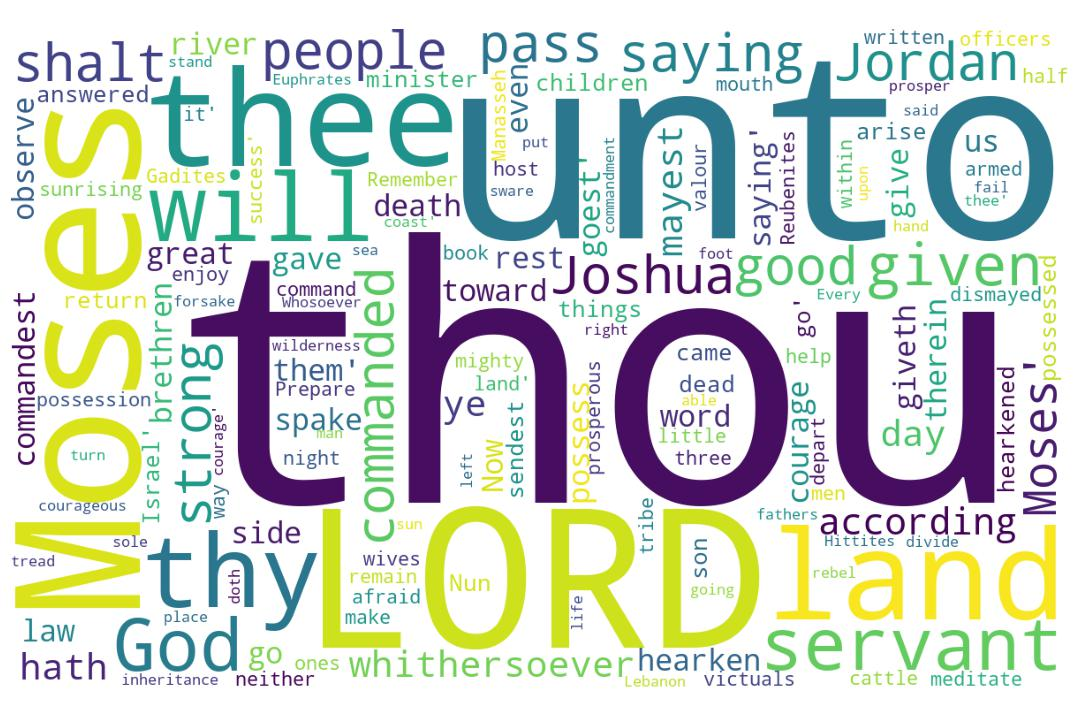
\includegraphics[width=\linewidth]{06OT-Joshua/Joshua1-WordCloud.jpg}
  \caption{Joshua 1 Word Cloud}
  \label{fig:Joshua 1 Word Cloud}
\end{figure}


\marginpar{\scriptsize \centering \fcolorbox{bone}{lime}{\textbf{NEW LEADER, WAITING LAND}}\\ (Joshua 1:1-18) \begin{compactenum}[I.][8]
    \item A \textbf{Son and his Legacy} \index[scripture]{Joshua!Jsh 01:01}(Jsh 1:1)
    \item A \textbf{Servant of the Lord} \index[scripture]{Joshua!Jsh 01:01}\index[scripture]{Joshua!Jsh 01:02}\index[scripture]{Joshua!Jsh 01:07}\index[scripture]{Joshua!Jsh 01:13}\index[scripture]{Joshua!Jsh 01:15}  (Jsh 1:1, 2, 7, 13, 15)
    \item Joshua \textbf{Assured for Life} \index[scripture]{Joshua!Jsh 01:05}(Jsh 1:5)
    \item  \textbf{Strength from the Law}  \index[scripture]{Joshua!Jsh 01:07}(Jsh 1:7)
    \item  \textbf{Success Limited} by adherence to the Law \index[scripture]{Joshua!Jsh 01:08}(Jsh 1:8)
    \item  \textbf{Sayings of a Leader} \index[scripture]{Joshua!Jsh 01:10} \index[scripture]{Joshua!Jsh 01:11}\index[scripture]{Joshua!Jsh 01:12}\index[scripture]{Joshua!Jsh 01:13}\index[scripture]{Joshua!Jsh 01:15} (Jsh 1:10, 11, 12, 13, 15)
    \item \textbf{Send us Into the Land!} \index[scripture]{Joshua!Jsh 01:16}(Jsh 1:16)
\end{compactenum}}

\footnote{\textcolor[cmyk]{0.99998,1,0,0}{\hyperlink{TOC}{Return to end of Table of Contents.}}}\footnote{\href{https://audiobible.com/bible/joshua_1.html}{\textcolor[cmyk]{0.99998,1,0,0}{Joshua Audio}}}\textcolor[cmyk]{0.99998,1,0,0}{Now after the death of Moses the \fcolorbox{bone}{lime}{servant of the LORD} it came to pass, that the LORD spake unto Joshua the \fcolorbox{bone}{lime}{son of Nun}, Moses' minister, saying,}
[2] \textcolor[cmyk]{0.99998,1,0,0}{Moses my \fcolorbox{bone}{lime}{servant} is dead; now therefore arise, go over this Jordan, thou, and all this people, unto the land which I do give to them, \emph{even} to the children of Israel.}
[3] \textcolor[cmyk]{0.99998,1,0,0}{Every place that the sole of your foot shall tread upon, that have I given unto you, as I said unto Moses.}
[4] \textcolor[cmyk]{0.99998,1,0,0}{From the wilderness and this Lebanon even unto the great river, the river Euphrates, all the land of the Hittites, and unto the great sea toward the going down of the sun, shall be your coast.}
[5] \textcolor[cmyk]{0.99998,1,0,0}{There shall not any man be able to stand before thee all the days of thy life: as I was with Moses, \emph{so} I will be with thee: I \fcolorbox{bone}{lime}{will not fail thee}, nor forsake thee.}
[6] \textcolor[cmyk]{0.99998,1,0,0}{Be strong and of a good courage: for unto this people shalt thou divide for an inheritance the land, which I sware unto their fathers to give them.}
[7] \textcolor[cmyk]{0.99998,1,0,0}{Only be thou \fcolorbox{bone}{lime}{strong} and very courageous, that thou mayest observe to do according to all the law, which Moses my \fcolorbox{bone}{lime}{servant} commanded thee: turn not from it \emph{to} the right hand or \emph{to} the left, that thou mayest prosper ommanded me, that ye should do so in the land whither ye go to possess it.}
[8] \textcolor[cmyk]{0.99998,1,0,0}{This book of the law shall not depart out of thy mouth; but thou shalt meditate therein day and night, that thou mayest observe to do according to all that is written therein: for then thou shalt make thy way prosperous, and then thou shalt have good \fcolorbox{bone}{lime}{success}.}
[9] \textcolor[cmyk]{0.99998,1,0,0}{Have not I commanded thee? Be strong and of a good courage; be not afraid, neither be thou dismayed: for the LORD thy God \emph{is} with thee whithersoever thou goest.}\\
\\
\P \textcolor[cmyk]{0.99998,1,0,0}{Then Joshua commanded the officers of the people, \fcolorbox{bone}{lime}{saying},}
[11] \textcolor[cmyk]{0.99998,1,0,0}{Pass through the host, and command the people, saying, Prepare you victuals; for within three days ye shall pass over this Jordan, to go in to possess the land, which the LORD your God giveth you to possess it.}\\
\\
\P \textcolor[cmyk]{0.99998,1,0,0}{And to the Reubenites, and to the Gadites, and to half the tribe of Manasseh, spake Joshua, saying,}
[13] \textcolor[cmyk]{0.99998,1,0,0}{Remember the word which Moses the \fcolorbox{bone}{lime}{servant} of the LORD commanded you, saying, The LORD your God hath given you rest, and hath given you this land.}
[14] \textcolor[cmyk]{0.99998,1,0,0}{Your wives, your little ones, and your cattle, shall remain in the land which Moses gave you on this side Jordan; but ye shall pass before your brethren armed, all the mighty men of valour, and help them;}
[15] \textcolor[cmyk]{0.99998,1,0,0}{Until the LORD have given your brethren rest, as \emph{he} \emph{hath} \emph{given} you, and they also have possessed the land which the LORD your God giveth them: then ye shall \fcolorbox{bone}{lime}{return} unto the land of your possession, and enjoy it, which Moses the LORD'S \fcolorbox{bone}{lime}{servant} gave you on this side Jordan toward the sunrising.}\\
\\
\P \textcolor[cmyk]{0.99998,1,0,0}{And they answered Joshua, saying, All that thou commandest us we will do, and whithersoever thou sendest us, we will go.}
[17] \textcolor[cmyk]{0.99998,1,0,0}{According as we hearkened unto Moses in all things, so will we hearken unto thee: only the LORD thy God be with thee, as he was with Moses.}
[18] \textcolor[cmyk]{0.99998,1,0,0}{Whosoever \emph{he} \emph{be} that doth rebel against thy commandment, and will not hearken unto thy words in all that thou commandest him, he shall be put to death: only be strong and of a good courage.}


\index[NWIV]{28!Joshua!Jos 1:1}\index[AWIP]{Now!Joshua!Jos 1:1}\index[AWIP]{after!Joshua!Jos 1:1}\index[AWIP]{the!Joshua!Jos 1:1}\index[AWIP]{the!Joshua!Jos 1:1 (2)}\index[AWIP]{the!Joshua!Jos 1:1 (3)}\index[AWIP]{the!Joshua!Jos 1:1 (4)}\index[AWIP]{the!Joshua!Jos 1:1 (5)}\index[AWIP]{death!Joshua!Jos 1:1}\index[AWIP]{of!Joshua!Jos 1:1}\index[AWIP]{of!Joshua!Jos 1:1 (2)}\index[AWIP]{of!Joshua!Jos 1:1 (3)}\index[AWIP]{Moses!Joshua!Jos 1:1}\index[AWIP]{servant!Joshua!Jos 1:1}\index[AWIP]{LORD!Joshua!Jos 1:1}\index[AWIP]{LORD!Joshua!Jos 1:1 (2)}\index[AWIP]{it!Joshua!Jos 1:1}\index[AWIP]{came!Joshua!Jos 1:1}\index[AWIP]{to!Joshua!Jos 1:1}\index[AWIP]{pass!Joshua!Jos 1:1}\index[AWIP]{that!Joshua!Jos 1:1}\index[AWIP]{spake!Joshua!Jos 1:1}\index[AWIP]{unto!Joshua!Jos 1:1}\index[AWIP]{Joshua!Joshua!Jos 1:1}\index[AWIP]{son!Joshua!Jos 1:1}\index[AWIP]{Nun!Joshua!Jos 1:1}\index[AWIP]{Moses'!Joshua!Jos 1:1}\index[AWIP]{minister!Joshua!Jos 1:1}\index[AWIP]{saying!Joshua!Jos 1:1}

\index[NWIV]{32!Joshua!Jos 1:2}\index[AWIP]{Moses!Joshua!Jos 1:2}\index[AWIP]{my!Joshua!Jos 1:2}\index[AWIP]{servant!Joshua!Jos 1:2}\index[AWIP]{is!Joshua!Jos 1:2}\index[AWIP]{dead!Joshua!Jos 1:2}\index[AWIP]{now!Joshua!Jos 1:2}\index[AWIP]{therefore!Joshua!Jos 1:2}\index[AWIP]{arise!Joshua!Jos 1:2}\index[AWIP]{go!Joshua!Jos 1:2}\index[AWIP]{over!Joshua!Jos 1:2}\index[AWIP]{this!Joshua!Jos 1:2}\index[AWIP]{this!Joshua!Jos 1:2 (2)}\index[AWIP]{Jordan!Joshua!Jos 1:2}\index[AWIP]{thou!Joshua!Jos 1:2}\index[AWIP]{and!Joshua!Jos 1:2}\index[AWIP]{all!Joshua!Jos 1:2}\index[AWIP]{people!Joshua!Jos 1:2}\index[AWIP]{unto!Joshua!Jos 1:2}\index[AWIP]{the!Joshua!Jos 1:2}\index[AWIP]{the!Joshua!Jos 1:2 (2)}\index[AWIP]{land!Joshua!Jos 1:2}\index[AWIP]{which!Joshua!Jos 1:2}\index[AWIP]{I!Joshua!Jos 1:2}\index[AWIP]{do!Joshua!Jos 1:2}\index[AWIP]{give!Joshua!Jos 1:2}\index[AWIP]{to!Joshua!Jos 1:2}\index[AWIP]{to!Joshua!Jos 1:2 (2)}\index[AWIP]{them!Joshua!Jos 1:2}\index[AWIP]{\emph{even}!Joshua!Jos 1:2}\index[AWIP]{children!Joshua!Jos 1:2}\index[AWIP]{of!Joshua!Jos 1:2}\index[AWIP]{Israel!Joshua!Jos 1:2}\index[AWIP]{\emph{even}!Joshua!Jos 1:2}

\index[NWIV]{22!Joshua!Jos 1:3}\index[AWIP]{Every!Joshua!Jos 1:3}\index[AWIP]{place!Joshua!Jos 1:3}\index[AWIP]{that!Joshua!Jos 1:3}\index[AWIP]{that!Joshua!Jos 1:3 (2)}\index[AWIP]{the!Joshua!Jos 1:3}\index[AWIP]{sole!Joshua!Jos 1:3}\index[AWIP]{of!Joshua!Jos 1:3}\index[AWIP]{your!Joshua!Jos 1:3}\index[AWIP]{foot!Joshua!Jos 1:3}\index[AWIP]{shall!Joshua!Jos 1:3}\index[AWIP]{tread!Joshua!Jos 1:3}\index[AWIP]{upon!Joshua!Jos 1:3}\index[AWIP]{have!Joshua!Jos 1:3}\index[AWIP]{I!Joshua!Jos 1:3}\index[AWIP]{I!Joshua!Jos 1:3 (2)}\index[AWIP]{given!Joshua!Jos 1:3}\index[AWIP]{unto!Joshua!Jos 1:3}\index[AWIP]{unto!Joshua!Jos 1:3 (2)}\index[AWIP]{you!Joshua!Jos 1:3}\index[AWIP]{as!Joshua!Jos 1:3}\index[AWIP]{said!Joshua!Jos 1:3}\index[AWIP]{Moses!Joshua!Jos 1:3}

\index[NWIV]{36!Joshua!Jos 1:4}\index[AWIP]{From!Joshua!Jos 1:4}\index[AWIP]{the!Joshua!Jos 1:4}\index[AWIP]{the!Joshua!Jos 1:4 (2)}\index[AWIP]{the!Joshua!Jos 1:4 (3)}\index[AWIP]{the!Joshua!Jos 1:4 (4)}\index[AWIP]{the!Joshua!Jos 1:4 (5)}\index[AWIP]{the!Joshua!Jos 1:4 (6)}\index[AWIP]{the!Joshua!Jos 1:4 (7)}\index[AWIP]{the!Joshua!Jos 1:4 (8)}\index[AWIP]{wilderness!Joshua!Jos 1:4}\index[AWIP]{and!Joshua!Jos 1:4}\index[AWIP]{and!Joshua!Jos 1:4 (2)}\index[AWIP]{this!Joshua!Jos 1:4}\index[AWIP]{Lebanon!Joshua!Jos 1:4}\index[AWIP]{even!Joshua!Jos 1:4}\index[AWIP]{unto!Joshua!Jos 1:4}\index[AWIP]{unto!Joshua!Jos 1:4 (2)}\index[AWIP]{great!Joshua!Jos 1:4}\index[AWIP]{great!Joshua!Jos 1:4 (2)}\index[AWIP]{river!Joshua!Jos 1:4}\index[AWIP]{river!Joshua!Jos 1:4 (2)}\index[AWIP]{Euphrates!Joshua!Jos 1:4}\index[AWIP]{all!Joshua!Jos 1:4}\index[AWIP]{land!Joshua!Jos 1:4}\index[AWIP]{of!Joshua!Jos 1:4}\index[AWIP]{of!Joshua!Jos 1:4 (2)}\index[AWIP]{Hittites!Joshua!Jos 1:4}\index[AWIP]{sea!Joshua!Jos 1:4}\index[AWIP]{toward!Joshua!Jos 1:4}\index[AWIP]{going!Joshua!Jos 1:4}\index[AWIP]{down!Joshua!Jos 1:4}\index[AWIP]{sun!Joshua!Jos 1:4}\index[AWIP]{shall!Joshua!Jos 1:4}\index[AWIP]{be!Joshua!Jos 1:4}\index[AWIP]{your!Joshua!Jos 1:4}\index[AWIP]{coast!Joshua!Jos 1:4}

\index[NWIV]{36!Joshua!Jos 1:5}\index[AWIP]{There!Joshua!Jos 1:5}\index[AWIP]{shall!Joshua!Jos 1:5}\index[AWIP]{not!Joshua!Jos 1:5}\index[AWIP]{not!Joshua!Jos 1:5 (2)}\index[AWIP]{any!Joshua!Jos 1:5}\index[AWIP]{man!Joshua!Jos 1:5}\index[AWIP]{be!Joshua!Jos 1:5}\index[AWIP]{be!Joshua!Jos 1:5 (2)}\index[AWIP]{able!Joshua!Jos 1:5}\index[AWIP]{to!Joshua!Jos 1:5}\index[AWIP]{stand!Joshua!Jos 1:5}\index[AWIP]{before!Joshua!Jos 1:5}\index[AWIP]{thee!Joshua!Jos 1:5}\index[AWIP]{thee!Joshua!Jos 1:5 (2)}\index[AWIP]{thee!Joshua!Jos 1:5 (3)}\index[AWIP]{thee!Joshua!Jos 1:5 (4)}\index[AWIP]{all!Joshua!Jos 1:5}\index[AWIP]{the!Joshua!Jos 1:5}\index[AWIP]{days!Joshua!Jos 1:5}\index[AWIP]{of!Joshua!Jos 1:5}\index[AWIP]{thy!Joshua!Jos 1:5}\index[AWIP]{life!Joshua!Jos 1:5}\index[AWIP]{as!Joshua!Jos 1:5}\index[AWIP]{I!Joshua!Jos 1:5}\index[AWIP]{I!Joshua!Jos 1:5 (2)}\index[AWIP]{I!Joshua!Jos 1:5 (3)}\index[AWIP]{was!Joshua!Jos 1:5}\index[AWIP]{with!Joshua!Jos 1:5}\index[AWIP]{with!Joshua!Jos 1:5 (2)}\index[AWIP]{Moses!Joshua!Jos 1:5}\index[AWIP]{\emph{so}!Joshua!Jos 1:5}\index[AWIP]{will!Joshua!Jos 1:5}\index[AWIP]{will!Joshua!Jos 1:5 (2)}\index[AWIP]{fail!Joshua!Jos 1:5}\index[AWIP]{nor!Joshua!Jos 1:5}\index[AWIP]{forsake!Joshua!Jos 1:5}\index[AWIP]{\emph{so}!Joshua!Jos 1:5}

\index[NWIV]{28!Joshua!Jos 1:6}\index[AWIP]{Be!Joshua!Jos 1:6}\index[AWIP]{strong!Joshua!Jos 1:6}\index[AWIP]{and!Joshua!Jos 1:6}\index[AWIP]{of!Joshua!Jos 1:6}\index[AWIP]{a!Joshua!Jos 1:6}\index[AWIP]{good!Joshua!Jos 1:6}\index[AWIP]{courage!Joshua!Jos 1:6}\index[AWIP]{for!Joshua!Jos 1:6}\index[AWIP]{for!Joshua!Jos 1:6 (2)}\index[AWIP]{unto!Joshua!Jos 1:6}\index[AWIP]{unto!Joshua!Jos 1:6 (2)}\index[AWIP]{this!Joshua!Jos 1:6}\index[AWIP]{people!Joshua!Jos 1:6}\index[AWIP]{shalt!Joshua!Jos 1:6}\index[AWIP]{thou!Joshua!Jos 1:6}\index[AWIP]{divide!Joshua!Jos 1:6}\index[AWIP]{an!Joshua!Jos 1:6}\index[AWIP]{inheritance!Joshua!Jos 1:6}\index[AWIP]{the!Joshua!Jos 1:6}\index[AWIP]{land!Joshua!Jos 1:6}\index[AWIP]{which!Joshua!Jos 1:6}\index[AWIP]{I!Joshua!Jos 1:6}\index[AWIP]{sware!Joshua!Jos 1:6}\index[AWIP]{their!Joshua!Jos 1:6}\index[AWIP]{fathers!Joshua!Jos 1:6}\index[AWIP]{to!Joshua!Jos 1:6}\index[AWIP]{give!Joshua!Jos 1:6}\index[AWIP]{them!Joshua!Jos 1:6}

\index[NWIV]{43!Joshua!Jos 1:7}\index[AWIP]{Only!Joshua!Jos 1:7}\index[AWIP]{be!Joshua!Jos 1:7}\index[AWIP]{thou!Joshua!Jos 1:7}\index[AWIP]{thou!Joshua!Jos 1:7 (2)}\index[AWIP]{thou!Joshua!Jos 1:7 (3)}\index[AWIP]{thou!Joshua!Jos 1:7 (4)}\index[AWIP]{strong!Joshua!Jos 1:7}\index[AWIP]{and!Joshua!Jos 1:7}\index[AWIP]{very!Joshua!Jos 1:7}\index[AWIP]{courageous!Joshua!Jos 1:7}\index[AWIP]{that!Joshua!Jos 1:7}\index[AWIP]{that!Joshua!Jos 1:7 (2)}\index[AWIP]{mayest!Joshua!Jos 1:7}\index[AWIP]{mayest!Joshua!Jos 1:7 (2)}\index[AWIP]{observe!Joshua!Jos 1:7}\index[AWIP]{to!Joshua!Jos 1:7}\index[AWIP]{to!Joshua!Jos 1:7 (2)}\index[AWIP]{do!Joshua!Jos 1:7}\index[AWIP]{according!Joshua!Jos 1:7}\index[AWIP]{all!Joshua!Jos 1:7}\index[AWIP]{the!Joshua!Jos 1:7}\index[AWIP]{the!Joshua!Jos 1:7 (2)}\index[AWIP]{the!Joshua!Jos 1:7 (3)}\index[AWIP]{law!Joshua!Jos 1:7}\index[AWIP]{which!Joshua!Jos 1:7}\index[AWIP]{Moses!Joshua!Jos 1:7}\index[AWIP]{my!Joshua!Jos 1:7}\index[AWIP]{servant!Joshua!Jos 1:7}\index[AWIP]{commanded!Joshua!Jos 1:7}\index[AWIP]{thee!Joshua!Jos 1:7}\index[AWIP]{turn!Joshua!Jos 1:7}\index[AWIP]{not!Joshua!Jos 1:7}\index[AWIP]{from!Joshua!Jos 1:7}\index[AWIP]{it!Joshua!Jos 1:7}\index[AWIP]{\emph{to}!Joshua!Jos 1:7}\index[AWIP]{\emph{to}!Joshua!Jos 1:7 (2)}\index[AWIP]{right!Joshua!Jos 1:7}\index[AWIP]{hand!Joshua!Jos 1:7}\index[AWIP]{or!Joshua!Jos 1:7}\index[AWIP]{left!Joshua!Jos 1:7}\index[AWIP]{prosper!Joshua!Jos 1:7}\index[AWIP]{whithersoever!Joshua!Jos 1:7}\index[AWIP]{goest!Joshua!Jos 1:7}\index[AWIP]{\emph{to}!Joshua!Jos 1:7}\index[AWIP]{\emph{to}!Joshua!Jos 1:7 (2)}

\index[NWIV]{48!Joshua!Jos 1:8}\index[AWIP]{This!Joshua!Jos 1:8}\index[AWIP]{book!Joshua!Jos 1:8}\index[AWIP]{of!Joshua!Jos 1:8}\index[AWIP]{of!Joshua!Jos 1:8 (2)}\index[AWIP]{the!Joshua!Jos 1:8}\index[AWIP]{law!Joshua!Jos 1:8}\index[AWIP]{shall!Joshua!Jos 1:8}\index[AWIP]{not!Joshua!Jos 1:8}\index[AWIP]{depart!Joshua!Jos 1:8}\index[AWIP]{out!Joshua!Jos 1:8}\index[AWIP]{thy!Joshua!Jos 1:8}\index[AWIP]{thy!Joshua!Jos 1:8 (2)}\index[AWIP]{mouth!Joshua!Jos 1:8}\index[AWIP]{but!Joshua!Jos 1:8}\index[AWIP]{thou!Joshua!Jos 1:8}\index[AWIP]{thou!Joshua!Jos 1:8 (2)}\index[AWIP]{thou!Joshua!Jos 1:8 (3)}\index[AWIP]{thou!Joshua!Jos 1:8 (4)}\index[AWIP]{shalt!Joshua!Jos 1:8}\index[AWIP]{shalt!Joshua!Jos 1:8 (2)}\index[AWIP]{shalt!Joshua!Jos 1:8 (3)}\index[AWIP]{meditate!Joshua!Jos 1:8}\index[AWIP]{therein!Joshua!Jos 1:8}\index[AWIP]{therein!Joshua!Jos 1:8 (2)}\index[AWIP]{day!Joshua!Jos 1:8}\index[AWIP]{and!Joshua!Jos 1:8}\index[AWIP]{and!Joshua!Jos 1:8 (2)}\index[AWIP]{night!Joshua!Jos 1:8}\index[AWIP]{that!Joshua!Jos 1:8}\index[AWIP]{that!Joshua!Jos 1:8 (2)}\index[AWIP]{mayest!Joshua!Jos 1:8}\index[AWIP]{observe!Joshua!Jos 1:8}\index[AWIP]{to!Joshua!Jos 1:8}\index[AWIP]{to!Joshua!Jos 1:8 (2)}\index[AWIP]{do!Joshua!Jos 1:8}\index[AWIP]{according!Joshua!Jos 1:8}\index[AWIP]{all!Joshua!Jos 1:8}\index[AWIP]{is!Joshua!Jos 1:8}\index[AWIP]{written!Joshua!Jos 1:8}\index[AWIP]{for!Joshua!Jos 1:8}\index[AWIP]{then!Joshua!Jos 1:8}\index[AWIP]{then!Joshua!Jos 1:8 (2)}\index[AWIP]{make!Joshua!Jos 1:8}\index[AWIP]{way!Joshua!Jos 1:8}\index[AWIP]{prosperous!Joshua!Jos 1:8}\index[AWIP]{have!Joshua!Jos 1:8}\index[AWIP]{good!Joshua!Jos 1:8}\index[AWIP]{success!Joshua!Jos 1:8}

\index[NWIV]{30!Joshua!Jos 1:9}\index[AWIP]{Have!Joshua!Jos 1:9}\index[AWIP]{not!Joshua!Jos 1:9}\index[AWIP]{not!Joshua!Jos 1:9 (2)}\index[AWIP]{I!Joshua!Jos 1:9}\index[AWIP]{commanded!Joshua!Jos 1:9}\index[AWIP]{thee?!Joshua!Jos 1:9}\index[AWIP]{Be!Joshua!Jos 1:9}\index[AWIP]{strong!Joshua!Jos 1:9}\index[AWIP]{and!Joshua!Jos 1:9}\index[AWIP]{of!Joshua!Jos 1:9}\index[AWIP]{a!Joshua!Jos 1:9}\index[AWIP]{good!Joshua!Jos 1:9}\index[AWIP]{courage!Joshua!Jos 1:9}\index[AWIP]{be!Joshua!Jos 1:9}\index[AWIP]{be!Joshua!Jos 1:9 (2)}\index[AWIP]{afraid!Joshua!Jos 1:9}\index[AWIP]{neither!Joshua!Jos 1:9}\index[AWIP]{thou!Joshua!Jos 1:9}\index[AWIP]{thou!Joshua!Jos 1:9 (2)}\index[AWIP]{dismayed!Joshua!Jos 1:9}\index[AWIP]{for!Joshua!Jos 1:9}\index[AWIP]{the!Joshua!Jos 1:9}\index[AWIP]{LORD!Joshua!Jos 1:9}\index[AWIP]{thy!Joshua!Jos 1:9}\index[AWIP]{God!Joshua!Jos 1:9}\index[AWIP]{\emph{is}!Joshua!Jos 1:9}\index[AWIP]{with!Joshua!Jos 1:9}\index[AWIP]{thee!Joshua!Jos 1:9}\index[AWIP]{whithersoever!Joshua!Jos 1:9}\index[AWIP]{goest!Joshua!Jos 1:9}\index[AWIP]{\emph{is}!Joshua!Jos 1:9}

\index[NWIV]{9!Joshua!Jos 1:10}\index[AWIP]{Then!Joshua!Jos 1:10}\index[AWIP]{Joshua!Joshua!Jos 1:10}\index[AWIP]{commanded!Joshua!Jos 1:10}\index[AWIP]{the!Joshua!Jos 1:10}\index[AWIP]{the!Joshua!Jos 1:10 (2)}\index[AWIP]{officers!Joshua!Jos 1:10}\index[AWIP]{of!Joshua!Jos 1:10}\index[AWIP]{people!Joshua!Jos 1:10}\index[AWIP]{saying!Joshua!Jos 1:10}

\index[NWIV]{39!Joshua!Jos 1:11}\index[AWIP]{Pass!Joshua!Jos 1:11}\index[AWIP]{through!Joshua!Jos 1:11}\index[AWIP]{the!Joshua!Jos 1:11}\index[AWIP]{the!Joshua!Jos 1:11 (2)}\index[AWIP]{the!Joshua!Jos 1:11 (3)}\index[AWIP]{the!Joshua!Jos 1:11 (4)}\index[AWIP]{host!Joshua!Jos 1:11}\index[AWIP]{and!Joshua!Jos 1:11}\index[AWIP]{command!Joshua!Jos 1:11}\index[AWIP]{people!Joshua!Jos 1:11}\index[AWIP]{saying!Joshua!Jos 1:11}\index[AWIP]{Prepare!Joshua!Jos 1:11}\index[AWIP]{you!Joshua!Jos 1:11}\index[AWIP]{you!Joshua!Jos 1:11 (2)}\index[AWIP]{victuals!Joshua!Jos 1:11}\index[AWIP]{for!Joshua!Jos 1:11}\index[AWIP]{within!Joshua!Jos 1:11}\index[AWIP]{three!Joshua!Jos 1:11}\index[AWIP]{days!Joshua!Jos 1:11}\index[AWIP]{ye!Joshua!Jos 1:11}\index[AWIP]{shall!Joshua!Jos 1:11}\index[AWIP]{pass!Joshua!Jos 1:11}\index[AWIP]{over!Joshua!Jos 1:11}\index[AWIP]{this!Joshua!Jos 1:11}\index[AWIP]{Jordan!Joshua!Jos 1:11}\index[AWIP]{to!Joshua!Jos 1:11}\index[AWIP]{to!Joshua!Jos 1:11 (2)}\index[AWIP]{to!Joshua!Jos 1:11 (3)}\index[AWIP]{go!Joshua!Jos 1:11}\index[AWIP]{in!Joshua!Jos 1:11}\index[AWIP]{possess!Joshua!Jos 1:11}\index[AWIP]{possess!Joshua!Jos 1:11 (2)}\index[AWIP]{land!Joshua!Jos 1:11}\index[AWIP]{which!Joshua!Jos 1:11}\index[AWIP]{LORD!Joshua!Jos 1:11}\index[AWIP]{your!Joshua!Jos 1:11}\index[AWIP]{God!Joshua!Jos 1:11}\index[AWIP]{giveth!Joshua!Jos 1:11}\index[AWIP]{it!Joshua!Jos 1:11}

\index[NWIV]{18!Joshua!Jos 1:12}\index[AWIP]{And!Joshua!Jos 1:12}\index[AWIP]{to!Joshua!Jos 1:12}\index[AWIP]{to!Joshua!Jos 1:12 (2)}\index[AWIP]{to!Joshua!Jos 1:12 (3)}\index[AWIP]{the!Joshua!Jos 1:12}\index[AWIP]{the!Joshua!Jos 1:12 (2)}\index[AWIP]{the!Joshua!Jos 1:12 (3)}\index[AWIP]{Reubenites!Joshua!Jos 1:12}\index[AWIP]{and!Joshua!Jos 1:12}\index[AWIP]{and!Joshua!Jos 1:12 (2)}\index[AWIP]{Gadites!Joshua!Jos 1:12}\index[AWIP]{half!Joshua!Jos 1:12}\index[AWIP]{tribe!Joshua!Jos 1:12}\index[AWIP]{of!Joshua!Jos 1:12}\index[AWIP]{Manasseh!Joshua!Jos 1:12}\index[AWIP]{spake!Joshua!Jos 1:12}\index[AWIP]{Joshua!Joshua!Jos 1:12}\index[AWIP]{saying!Joshua!Jos 1:12}

\index[NWIV]{27!Joshua!Jos 1:13}\index[AWIP]{Remember!Joshua!Jos 1:13}\index[AWIP]{the!Joshua!Jos 1:13}\index[AWIP]{the!Joshua!Jos 1:13 (2)}\index[AWIP]{the!Joshua!Jos 1:13 (3)}\index[AWIP]{word!Joshua!Jos 1:13}\index[AWIP]{which!Joshua!Jos 1:13}\index[AWIP]{Moses!Joshua!Jos 1:13}\index[AWIP]{servant!Joshua!Jos 1:13}\index[AWIP]{of!Joshua!Jos 1:13}\index[AWIP]{LORD!Joshua!Jos 1:13}\index[AWIP]{LORD!Joshua!Jos 1:13 (2)}\index[AWIP]{commanded!Joshua!Jos 1:13}\index[AWIP]{you!Joshua!Jos 1:13}\index[AWIP]{you!Joshua!Jos 1:13 (2)}\index[AWIP]{you!Joshua!Jos 1:13 (3)}\index[AWIP]{saying!Joshua!Jos 1:13}\index[AWIP]{The!Joshua!Jos 1:13}\index[AWIP]{your!Joshua!Jos 1:13}\index[AWIP]{God!Joshua!Jos 1:13}\index[AWIP]{hath!Joshua!Jos 1:13}\index[AWIP]{hath!Joshua!Jos 1:13 (2)}\index[AWIP]{given!Joshua!Jos 1:13}\index[AWIP]{given!Joshua!Jos 1:13 (2)}\index[AWIP]{rest!Joshua!Jos 1:13}\index[AWIP]{and!Joshua!Jos 1:13}\index[AWIP]{this!Joshua!Jos 1:13}\index[AWIP]{land!Joshua!Jos 1:13}

\index[NWIV]{38!Joshua!Jos 1:14}\index[AWIP]{Your!Joshua!Jos 1:14}\index[AWIP]{wives!Joshua!Jos 1:14}\index[AWIP]{your!Joshua!Jos 1:14}\index[AWIP]{your!Joshua!Jos 1:14 (2)}\index[AWIP]{your!Joshua!Jos 1:14 (3)}\index[AWIP]{little!Joshua!Jos 1:14}\index[AWIP]{ones!Joshua!Jos 1:14}\index[AWIP]{and!Joshua!Jos 1:14}\index[AWIP]{and!Joshua!Jos 1:14 (2)}\index[AWIP]{cattle!Joshua!Jos 1:14}\index[AWIP]{shall!Joshua!Jos 1:14}\index[AWIP]{shall!Joshua!Jos 1:14 (2)}\index[AWIP]{remain!Joshua!Jos 1:14}\index[AWIP]{in!Joshua!Jos 1:14}\index[AWIP]{the!Joshua!Jos 1:14}\index[AWIP]{the!Joshua!Jos 1:14 (2)}\index[AWIP]{land!Joshua!Jos 1:14}\index[AWIP]{which!Joshua!Jos 1:14}\index[AWIP]{Moses!Joshua!Jos 1:14}\index[AWIP]{gave!Joshua!Jos 1:14}\index[AWIP]{you!Joshua!Jos 1:14}\index[AWIP]{on!Joshua!Jos 1:14}\index[AWIP]{this!Joshua!Jos 1:14}\index[AWIP]{side!Joshua!Jos 1:14}\index[AWIP]{Jordan!Joshua!Jos 1:14}\index[AWIP]{but!Joshua!Jos 1:14}\index[AWIP]{ye!Joshua!Jos 1:14}\index[AWIP]{pass!Joshua!Jos 1:14}\index[AWIP]{before!Joshua!Jos 1:14}\index[AWIP]{brethren!Joshua!Jos 1:14}\index[AWIP]{armed!Joshua!Jos 1:14}\index[AWIP]{all!Joshua!Jos 1:14}\index[AWIP]{mighty!Joshua!Jos 1:14}\index[AWIP]{men!Joshua!Jos 1:14}\index[AWIP]{of!Joshua!Jos 1:14}\index[AWIP]{valour!Joshua!Jos 1:14}\index[AWIP]{help!Joshua!Jos 1:14}\index[AWIP]{them!Joshua!Jos 1:14}

\index[NWIV]{54!Joshua!Jos 1:15}\index[AWIP]{Until!Joshua!Jos 1:15}\index[AWIP]{the!Joshua!Jos 1:15}\index[AWIP]{the!Joshua!Jos 1:15 (2)}\index[AWIP]{the!Joshua!Jos 1:15 (3)}\index[AWIP]{the!Joshua!Jos 1:15 (4)}\index[AWIP]{the!Joshua!Jos 1:15 (5)}\index[AWIP]{the!Joshua!Jos 1:15 (6)}\index[AWIP]{LORD!Joshua!Jos 1:15}\index[AWIP]{LORD!Joshua!Jos 1:15 (2)}\index[AWIP]{have!Joshua!Jos 1:15}\index[AWIP]{have!Joshua!Jos 1:15 (2)}\index[AWIP]{given!Joshua!Jos 1:15}\index[AWIP]{your!Joshua!Jos 1:15}\index[AWIP]{your!Joshua!Jos 1:15 (2)}\index[AWIP]{your!Joshua!Jos 1:15 (3)}\index[AWIP]{brethren!Joshua!Jos 1:15}\index[AWIP]{rest!Joshua!Jos 1:15}\index[AWIP]{as!Joshua!Jos 1:15}\index[AWIP]{\emph{he}!Joshua!Jos 1:15}\index[AWIP]{\emph{hath}!Joshua!Jos 1:15}\index[AWIP]{\emph{given}!Joshua!Jos 1:15}\index[AWIP]{you!Joshua!Jos 1:15}\index[AWIP]{you!Joshua!Jos 1:15 (2)}\index[AWIP]{and!Joshua!Jos 1:15}\index[AWIP]{and!Joshua!Jos 1:15 (2)}\index[AWIP]{they!Joshua!Jos 1:15}\index[AWIP]{also!Joshua!Jos 1:15}\index[AWIP]{possessed!Joshua!Jos 1:15}\index[AWIP]{land!Joshua!Jos 1:15}\index[AWIP]{land!Joshua!Jos 1:15 (2)}\index[AWIP]{which!Joshua!Jos 1:15}\index[AWIP]{which!Joshua!Jos 1:15 (2)}\index[AWIP]{God!Joshua!Jos 1:15}\index[AWIP]{giveth!Joshua!Jos 1:15}\index[AWIP]{them!Joshua!Jos 1:15}\index[AWIP]{then!Joshua!Jos 1:15}\index[AWIP]{ye!Joshua!Jos 1:15}\index[AWIP]{shall!Joshua!Jos 1:15}\index[AWIP]{return!Joshua!Jos 1:15}\index[AWIP]{unto!Joshua!Jos 1:15}\index[AWIP]{of!Joshua!Jos 1:15}\index[AWIP]{possession!Joshua!Jos 1:15}\index[AWIP]{enjoy!Joshua!Jos 1:15}\index[AWIP]{it!Joshua!Jos 1:15}\index[AWIP]{Moses!Joshua!Jos 1:15}\index[AWIP]{LORD'S!Joshua!Jos 1:15}\index[AWIP]{servant!Joshua!Jos 1:15}\index[AWIP]{gave!Joshua!Jos 1:15}\index[AWIP]{on!Joshua!Jos 1:15}\index[AWIP]{this!Joshua!Jos 1:15}\index[AWIP]{side!Joshua!Jos 1:15}\index[AWIP]{Jordan!Joshua!Jos 1:15}\index[AWIP]{toward!Joshua!Jos 1:15}\index[AWIP]{sunrising!Joshua!Jos 1:15}\index[AWIP]{\emph{he}!Joshua!Jos 1:15}\index[AWIP]{\emph{hath}!Joshua!Jos 1:15}\index[AWIP]{\emph{given}!Joshua!Jos 1:15}

\index[NWIV]{21!Joshua!Jos 1:16}\index[AWIP]{And!Joshua!Jos 1:16}\index[AWIP]{they!Joshua!Jos 1:16}\index[AWIP]{answered!Joshua!Jos 1:16}\index[AWIP]{Joshua!Joshua!Jos 1:16}\index[AWIP]{saying!Joshua!Jos 1:16}\index[AWIP]{All!Joshua!Jos 1:16}\index[AWIP]{that!Joshua!Jos 1:16}\index[AWIP]{thou!Joshua!Jos 1:16}\index[AWIP]{thou!Joshua!Jos 1:16 (2)}\index[AWIP]{commandest!Joshua!Jos 1:16}\index[AWIP]{us!Joshua!Jos 1:16}\index[AWIP]{us!Joshua!Jos 1:16 (2)}\index[AWIP]{we!Joshua!Jos 1:16}\index[AWIP]{we!Joshua!Jos 1:16 (2)}\index[AWIP]{will!Joshua!Jos 1:16}\index[AWIP]{will!Joshua!Jos 1:16 (2)}\index[AWIP]{do!Joshua!Jos 1:16}\index[AWIP]{and!Joshua!Jos 1:16}\index[AWIP]{whithersoever!Joshua!Jos 1:16}\index[AWIP]{sendest!Joshua!Jos 1:16}\index[AWIP]{go!Joshua!Jos 1:16}

\index[NWIV]{28!Joshua!Jos 1:17}\index[AWIP]{According!Joshua!Jos 1:17}\index[AWIP]{as!Joshua!Jos 1:17}\index[AWIP]{as!Joshua!Jos 1:17 (2)}\index[AWIP]{we!Joshua!Jos 1:17}\index[AWIP]{we!Joshua!Jos 1:17 (2)}\index[AWIP]{hearkened!Joshua!Jos 1:17}\index[AWIP]{unto!Joshua!Jos 1:17}\index[AWIP]{unto!Joshua!Jos 1:17 (2)}\index[AWIP]{Moses!Joshua!Jos 1:17}\index[AWIP]{Moses!Joshua!Jos 1:17 (2)}\index[AWIP]{in!Joshua!Jos 1:17}\index[AWIP]{all!Joshua!Jos 1:17}\index[AWIP]{things!Joshua!Jos 1:17}\index[AWIP]{so!Joshua!Jos 1:17}\index[AWIP]{will!Joshua!Jos 1:17}\index[AWIP]{hearken!Joshua!Jos 1:17}\index[AWIP]{thee!Joshua!Jos 1:17}\index[AWIP]{thee!Joshua!Jos 1:17 (2)}\index[AWIP]{only!Joshua!Jos 1:17}\index[AWIP]{the!Joshua!Jos 1:17}\index[AWIP]{LORD!Joshua!Jos 1:17}\index[AWIP]{thy!Joshua!Jos 1:17}\index[AWIP]{God!Joshua!Jos 1:17}\index[AWIP]{be!Joshua!Jos 1:17}\index[AWIP]{with!Joshua!Jos 1:17}\index[AWIP]{with!Joshua!Jos 1:17 (2)}\index[AWIP]{he!Joshua!Jos 1:17}\index[AWIP]{was!Joshua!Jos 1:17}

\index[NWIV]{36!Joshua!Jos 1:18}\index[AWIP]{Whosoever!Joshua!Jos 1:18}\index[AWIP]{\emph{he}!Joshua!Jos 1:18}\index[AWIP]{\emph{be}!Joshua!Jos 1:18}\index[AWIP]{that!Joshua!Jos 1:18}\index[AWIP]{that!Joshua!Jos 1:18 (2)}\index[AWIP]{doth!Joshua!Jos 1:18}\index[AWIP]{rebel!Joshua!Jos 1:18}\index[AWIP]{against!Joshua!Jos 1:18}\index[AWIP]{thy!Joshua!Jos 1:18}\index[AWIP]{thy!Joshua!Jos 1:18 (2)}\index[AWIP]{commandment!Joshua!Jos 1:18}\index[AWIP]{and!Joshua!Jos 1:18}\index[AWIP]{and!Joshua!Jos 1:18 (2)}\index[AWIP]{will!Joshua!Jos 1:18}\index[AWIP]{not!Joshua!Jos 1:18}\index[AWIP]{hearken!Joshua!Jos 1:18}\index[AWIP]{unto!Joshua!Jos 1:18}\index[AWIP]{words!Joshua!Jos 1:18}\index[AWIP]{in!Joshua!Jos 1:18}\index[AWIP]{all!Joshua!Jos 1:18}\index[AWIP]{thou!Joshua!Jos 1:18}\index[AWIP]{commandest!Joshua!Jos 1:18}\index[AWIP]{him!Joshua!Jos 1:18}\index[AWIP]{he!Joshua!Jos 1:18}\index[AWIP]{shall!Joshua!Jos 1:18}\index[AWIP]{be!Joshua!Jos 1:18}\index[AWIP]{be!Joshua!Jos 1:18 (2)}\index[AWIP]{put!Joshua!Jos 1:18}\index[AWIP]{to!Joshua!Jos 1:18}\index[AWIP]{death!Joshua!Jos 1:18}\index[AWIP]{only!Joshua!Jos 1:18}\index[AWIP]{strong!Joshua!Jos 1:18}\index[AWIP]{of!Joshua!Jos 1:18}\index[AWIP]{a!Joshua!Jos 1:18}\index[AWIP]{good!Joshua!Jos 1:18}\index[AWIP]{courage!Joshua!Jos 1:18}\index[AWIP]{\emph{he}!Joshua!Jos 1:18}\index[AWIP]{\emph{be}!Joshua!Jos 1:18}


\section{Joshua 1 Outlines}

\subsection{My Outlines}

\subsubsection{A New Leader, A Waiting Land}
\index[speaker]{Keith Anthony!Joshua 01 (A New Leader, A Waiting Land)}
\index[series]{Joshua (Keith Anthony)!Joshua 01 (A New Leader, A Waiting Land)}
\index[date]{2018/03/05!Joshua 01 (A New Leader, A Waiting Land) (Keith Anthony)}
\begin{compactenum}[I.]
    \item A \textbf{Son and his Legacy} \index[scripture]{Joshua!Jsh 01:01}(Jsh 1:1)
    \item A \textbf{Servant of the Lord} \index[scripture]{Joshua!Jsh 01:01}\index[scripture]{Joshua!Jsh 01:02}\index[scripture]{Joshua!Jsh 01:07}\index[scripture]{Joshua!Jsh 01:13}\index[scripture]{Joshua!Jsh 01:15}  (Jsh 1:1, 2, 7, 13, 15)
    \item Joshua \textbf{Assured for Life} \index[scripture]{Joshua!Jsh 01:05}(Jsh 1:5)
    \item  \textbf{Strength from the Law}  \index[scripture]{Joshua!Jsh 01:07}(Jsh 1:7)
    \item  \textbf{Success Limited} by adherence to the Law \index[scripture]{Joshua!Jsh 01:08}(Jsh 1:8)
    \item  \textbf{Sayings of a Leader} \index[scripture]{Joshua!Jsh 01:10} \index[scripture]{Joshua!Jsh 01:11}\index[scripture]{Joshua!Jsh 01:12}\index[scripture]{Joshua!Jsh 01:13}\index[scripture]{Joshua!Jsh 01:15} (Jsh 1:10, 11, 12, 13, 15)
    \item \textbf{Send us Into the Land!} \index[scripture]{Joshua!Jsh 01:16}(Jsh 1:16)
\end{compactenum}



\subsection{Outlines from Others}


\section{Joshua 1 Comments}



\chapter{Joshua 2}

\begin{figure}
  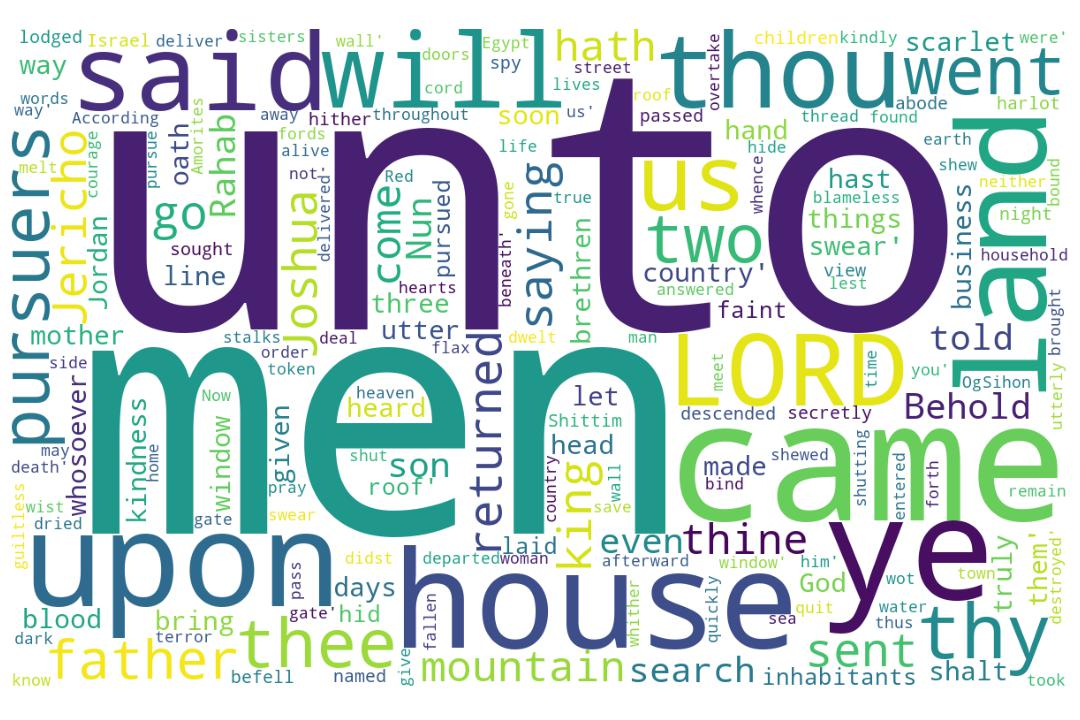
\includegraphics[width=\linewidth]{06OT-Joshua/Joshua2-WordCloud.jpg}
  \caption{Joshua 2 Word Cloud}
  \label{fig:Joshua 2 Word Cloud}
\end{figure}


\marginpar{\scriptsize \centering \fcolorbox{bone}{lime}{\textbf{MEET RAHAB}}\\ (Joshua 2:1-24) \begin{compactenum}[I.][8]
    \item A \textbf{Paradox} \index[scripture]{Joshua!Jsh 01:01--22}(Joshua 1:1--22) God has to work through the frailties an faults of mankind
    \item Rahab's  \textbf{Profession} \index[scripture]{Joshua!Jsh 02:01}(Jsh 2:1) 
    \item Rahab's  \textbf{Prominence} \index[scripture]{Joshua!Jsh 02:03}(Jsh 2:3) 
    \item Rahab's  \textbf{Prevarication} \index[scripture]{Joshua!Jsh 02:04}(Jsh 2:4) 
    \item Rahab's  \textbf{Promise} \index[scripture]{Joshua!Jsh 02:13}(Jsh 2:13) 
    \item Rahab's  \textbf{Paradigm} \index[scripture]{Matthew!Matt 21:31}(Matt 21:31) 
    \item Rahab's  \textbf{Progeny} \index[scripture]{Matthew!Matt 01:05--06}(Matt 1:5--6) 
\end{compactenum}}

\marginpar{\scriptsize \centering \fcolorbox{bone}{yellow}{\textbf{THE CONVERSION OF RAHAB}}\\ (Joshua 2:1-24) \begin{compactenum}[I.][8]
    \item The \textbf{Fib} \index[scripture]{Joshua!Jsh 01:04}(Jsh 1:4) 
    \item The \textbf{Flax} \index[scripture]{Joshua!Jsh 01:06}(Jsh 1:6) 
    \item The \textbf{Fords} \index[scripture]{Joshua!Jsh 01:07}(Jsh 1:7) 
    \item The \textbf{Fear} \index[scripture]{Joshua!Jsh 01:09}(Jsh 1:9) 
    \item The \textbf{Faith} \index[scripture]{Joshua!Jsh 01:11}(Jsh 1:11) 
    \item The \textbf{Family} \index[scripture]{Joshua!Jsh 01:13}(Jsh 1:13) 
    \item The \textbf{Fainting} \index[scripture]{Joshua!Jsh 01:24}(Jsh 1:24) 
\end{compactenum}}

\marginpar{\scriptsize \centering \fcolorbox{bone}{black}{\textbf{\textcolor{white}{RAHAB CHANGED}}}\\ (Joshua 2:1-24)\begin{compactenum}[I.]
    \item Rahab the \textbf{Harlot} \index[scripture]{Joshua!Jsh 01:02}(Jsh 1:2) 
    \item Rahab's  \textbf{Scarlet} \index[scripture]{Joshua!Jsh 01:18}(Jsh 1:18) 
    \item Rahab the  \textbf{Starlet!} \index[scripture]{Matthew!Matt 01:05--06}(Matt 1:5--6) 
\end{compactenum}}



\footnote{\textcolor[cmyk]{0.99998,1,0,0}{\hyperlink{TOC}{Return to end of Table of Contents.}}}\footnote{\href{https://audiobible.com/bible/joshua_1.html}{\textcolor[cmyk]{0.99998,1,0,0}{Joshua Audio}}}\textcolor[cmyk]{0.99998,1,0,0}{And Joshua the son of Nun sent out of Shittim two men to spy secretly, saying, Go view the land, even Jericho. And they went, and came into an \fcolorbox{bone}{lime}{harlot's} house, named Rahab, and lodged there.}
[2] \textcolor[cmyk]{0.99998,1,0,0}{And it was told the king of Jericho, saying, Behold, there came men in hither to night of the children of Israel to search out the country.}
[3] \textcolor[cmyk]{0.99998,1,0,0}{And the \fcolorbox{bone}{lime}{king of Jericho} sent unto Rahab, saying, Bring forth the men that are come to thee, which are entered into thine house: for they be come to search out all the country.}
[4] \textcolor[cmyk]{0.99998,1,0,0}{And the woman took the two men, and hid them, and said thus, There came men unto me, but I \fcolorbox{bone}{lime}{wist not} whence they \emph{were}:}
[5] \textcolor[cmyk]{0.99998,1,0,0}{And it came to pass \emph{about} \emph{the} \emph{time} of shutting of the gate, when it was dark, that the men went out: whither the men went I wot not: pursue after them quickly; for ye shall overtake them.}
[6] \textcolor[cmyk]{0.99998,1,0,0}{But she had brought them up to the roof of the house, and hid them with the stalks of flax, which she had laid in order upon the roof.}
[7] \textcolor[cmyk]{0.99998,1,0,0}{And the men pursued after them the way to Jordan unto the fords: and as soon as they which pursued after them were gone out, they shut the gate.}\\
\\
\P \textcolor[cmyk]{0.99998,1,0,0}{And before they were laid down, she came up unto them upon the roof;}
[9] \textcolor[cmyk]{0.99998,1,0,0}{And she said unto the men, I know that the LORD hath given you the land, and that your terror is fallen upon us, and that all the inhabitants of the land faint because of you.}
[10] \textcolor[cmyk]{0.99998,1,0,0}{For we have heard how the LORD dried up the water of the Red sea for you, when ye came out of Egypt; and what ye did unto the two kings of the Amorites, that \emph{were} on the other side Jordan, Sihon and Og, whom ye utterly destroyed.}
[11] \textcolor[cmyk]{0.99998,1,0,0}{And as soon as we had heard \emph{these} \emph{things}, our hearts did melt, neither did there remain any more courage in any man, because of you: for the LORD your God, he \emph{is} God in heaven above, and in earth beneath.}
[12] \textcolor[cmyk]{0.99998,1,0,0}{Now therefore, I pray you, swear unto me by the LORD, since I have shewed you kindness, that ye will also shew kindness unto my father's house, and give me a true token:}
[13] \textcolor[cmyk]{0.99998,1,0,0}{And \emph{that} ye will \fcolorbox{bone}{lime}{save alive} my father, and my mother, and my brethren, and my sisters, and all that they have, and deliver our lives from death.}
[14] \textcolor[cmyk]{0.99998,1,0,0}{And the men answered her, Our life for your's, if ye utter not this our business. And it shall be, when the LORD hath given us the land, that we will deal kindly and truly with thee.}
[15] \textcolor[cmyk]{0.99998,1,0,0}{Then she let them down by a cord through the window: for her house \emph{was} upon the town wall, and she dwelt upon the wall.}
[16] \textcolor[cmyk]{0.99998,1,0,0}{And she said unto them, Get you to the mountain, lest the pursuers meet you; and hide yourselves there three days, until the pursuers be returned: and afterward may ye go your way.}
[17] \textcolor[cmyk]{0.99998,1,0,0}{And the men said unto her, We \emph{will} \emph{be} blameless of this thine oath which thou hast made us swear.}
[18] \textcolor[cmyk]{0.99998,1,0,0}{Behold, \emph{when} we come into the land, thou shalt bind this line of scarlet thread in the window which thou didst let us down by: and thou shalt bring thy father, and thy mother, and thy brethren, and all thy father's household, home unto thee.}
[19] \textcolor[cmyk]{0.99998,1,0,0}{And it shall be, \emph{that} whosoever shall go out of the doors of thy house into the street, his blood \emph{shall} \emph{be} upon his head, and we \emph{will} \emph{be} guiltless: and whosoever shall be with thee in the house, his blood \emph{shall} \emph{be} on our head, if \emph{any} hand be upon him.}
[20] \textcolor[cmyk]{0.99998,1,0,0}{And if thou utter this our business, then we will be quit of thine oath which thou hast made us to swear.}
[21] \textcolor[cmyk]{0.99998,1,0,0}{And she said, According unto your words, so \emph{be} it. And she sent them away, and they departed: and she bound the scarlet line in the window.}
[22] \textcolor[cmyk]{0.99998,1,0,0}{And they went, and came unto the mountain, and abode there three days, until the pursuers were returned: and the pursuers sought \emph{them} throughout all the way, but found \emph{them} not.}\\
\\
\P \textcolor[cmyk]{0.99998,1,0,0}{So the two men returned, and descended from the mountain, and passed over, and came to Joshua the son of Nun, and told him all \emph{things} that befell them:}
[24] \textcolor[cmyk]{0.99998,1,0,0}{And they said unto Joshua, Truly the LORD hath delivered into our hands all the land; for even all the inhabitants of the country do faint because of us.}
\index[NWIV]{36!Joshua!Jos 2:1}\index[AWIP]{And!Joshua!Jos 2:1}\index[AWIP]{And!Joshua!Jos 2:1 (2)}\index[AWIP]{Joshua!Joshua!Jos 2:1}\index[AWIP]{the!Joshua!Jos 2:1}\index[AWIP]{the!Joshua!Jos 2:1 (2)}\index[AWIP]{son!Joshua!Jos 2:1}\index[AWIP]{of!Joshua!Jos 2:1}\index[AWIP]{of!Joshua!Jos 2:1 (2)}\index[AWIP]{Nun!Joshua!Jos 2:1}\index[AWIP]{sent!Joshua!Jos 2:1}\index[AWIP]{out!Joshua!Jos 2:1}\index[AWIP]{Shittim!Joshua!Jos 2:1}\index[AWIP]{two!Joshua!Jos 2:1}\index[AWIP]{men!Joshua!Jos 2:1}\index[AWIP]{to!Joshua!Jos 2:1}\index[AWIP]{spy!Joshua!Jos 2:1}\index[AWIP]{secretly!Joshua!Jos 2:1}\index[AWIP]{saying!Joshua!Jos 2:1}\index[AWIP]{Go!Joshua!Jos 2:1}\index[AWIP]{view!Joshua!Jos 2:1}\index[AWIP]{land!Joshua!Jos 2:1}\index[AWIP]{even!Joshua!Jos 2:1}\index[AWIP]{Jericho!Joshua!Jos 2:1}\index[AWIP]{they!Joshua!Jos 2:1}\index[AWIP]{went!Joshua!Jos 2:1}\index[AWIP]{and!Joshua!Jos 2:1}\index[AWIP]{and!Joshua!Jos 2:1 (2)}\index[AWIP]{came!Joshua!Jos 2:1}\index[AWIP]{into!Joshua!Jos 2:1}\index[AWIP]{an!Joshua!Jos 2:1}\index[AWIP]{harlot's!Joshua!Jos 2:1}\index[AWIP]{house!Joshua!Jos 2:1}\index[AWIP]{named!Joshua!Jos 2:1}\index[AWIP]{Rahab!Joshua!Jos 2:1}\index[AWIP]{lodged!Joshua!Jos 2:1}\index[AWIP]{there!Joshua!Jos 2:1}

\index[NWIV]{27!Joshua!Jos 2:2}\index[AWIP]{And!Joshua!Jos 2:2}\index[AWIP]{it!Joshua!Jos 2:2}\index[AWIP]{was!Joshua!Jos 2:2}\index[AWIP]{told!Joshua!Jos 2:2}\index[AWIP]{the!Joshua!Jos 2:2}\index[AWIP]{the!Joshua!Jos 2:2 (2)}\index[AWIP]{the!Joshua!Jos 2:2 (3)}\index[AWIP]{king!Joshua!Jos 2:2}\index[AWIP]{of!Joshua!Jos 2:2}\index[AWIP]{of!Joshua!Jos 2:2 (2)}\index[AWIP]{of!Joshua!Jos 2:2 (3)}\index[AWIP]{Jericho!Joshua!Jos 2:2}\index[AWIP]{saying!Joshua!Jos 2:2}\index[AWIP]{Behold!Joshua!Jos 2:2}\index[AWIP]{there!Joshua!Jos 2:2}\index[AWIP]{came!Joshua!Jos 2:2}\index[AWIP]{men!Joshua!Jos 2:2}\index[AWIP]{in!Joshua!Jos 2:2}\index[AWIP]{hither!Joshua!Jos 2:2}\index[AWIP]{to!Joshua!Jos 2:2}\index[AWIP]{to!Joshua!Jos 2:2 (2)}\index[AWIP]{night!Joshua!Jos 2:2}\index[AWIP]{children!Joshua!Jos 2:2}\index[AWIP]{Israel!Joshua!Jos 2:2}\index[AWIP]{search!Joshua!Jos 2:2}\index[AWIP]{out!Joshua!Jos 2:2}\index[AWIP]{country!Joshua!Jos 2:2}

\index[NWIV]{34!Joshua!Jos 2:3}\index[AWIP]{And!Joshua!Jos 2:3}\index[AWIP]{the!Joshua!Jos 2:3}\index[AWIP]{the!Joshua!Jos 2:3 (2)}\index[AWIP]{the!Joshua!Jos 2:3 (3)}\index[AWIP]{king!Joshua!Jos 2:3}\index[AWIP]{of!Joshua!Jos 2:3}\index[AWIP]{Jericho!Joshua!Jos 2:3}\index[AWIP]{sent!Joshua!Jos 2:3}\index[AWIP]{unto!Joshua!Jos 2:3}\index[AWIP]{Rahab!Joshua!Jos 2:3}\index[AWIP]{saying!Joshua!Jos 2:3}\index[AWIP]{Bring!Joshua!Jos 2:3}\index[AWIP]{forth!Joshua!Jos 2:3}\index[AWIP]{men!Joshua!Jos 2:3}\index[AWIP]{that!Joshua!Jos 2:3}\index[AWIP]{are!Joshua!Jos 2:3}\index[AWIP]{are!Joshua!Jos 2:3 (2)}\index[AWIP]{come!Joshua!Jos 2:3}\index[AWIP]{come!Joshua!Jos 2:3 (2)}\index[AWIP]{to!Joshua!Jos 2:3}\index[AWIP]{to!Joshua!Jos 2:3 (2)}\index[AWIP]{thee!Joshua!Jos 2:3}\index[AWIP]{which!Joshua!Jos 2:3}\index[AWIP]{entered!Joshua!Jos 2:3}\index[AWIP]{into!Joshua!Jos 2:3}\index[AWIP]{thine!Joshua!Jos 2:3}\index[AWIP]{house!Joshua!Jos 2:3}\index[AWIP]{for!Joshua!Jos 2:3}\index[AWIP]{they!Joshua!Jos 2:3}\index[AWIP]{be!Joshua!Jos 2:3}\index[AWIP]{search!Joshua!Jos 2:3}\index[AWIP]{out!Joshua!Jos 2:3}\index[AWIP]{all!Joshua!Jos 2:3}\index[AWIP]{country!Joshua!Jos 2:3}

\index[NWIV]{25!Joshua!Jos 2:4}\index[AWIP]{And!Joshua!Jos 2:4}\index[AWIP]{the!Joshua!Jos 2:4}\index[AWIP]{the!Joshua!Jos 2:4 (2)}\index[AWIP]{woman!Joshua!Jos 2:4}\index[AWIP]{took!Joshua!Jos 2:4}\index[AWIP]{two!Joshua!Jos 2:4}\index[AWIP]{men!Joshua!Jos 2:4}\index[AWIP]{men!Joshua!Jos 2:4 (2)}\index[AWIP]{and!Joshua!Jos 2:4}\index[AWIP]{and!Joshua!Jos 2:4 (2)}\index[AWIP]{hid!Joshua!Jos 2:4}\index[AWIP]{them!Joshua!Jos 2:4}\index[AWIP]{said!Joshua!Jos 2:4}\index[AWIP]{thus!Joshua!Jos 2:4}\index[AWIP]{There!Joshua!Jos 2:4}\index[AWIP]{came!Joshua!Jos 2:4}\index[AWIP]{unto!Joshua!Jos 2:4}\index[AWIP]{me!Joshua!Jos 2:4}\index[AWIP]{but!Joshua!Jos 2:4}\index[AWIP]{I!Joshua!Jos 2:4}\index[AWIP]{wist!Joshua!Jos 2:4}\index[AWIP]{not!Joshua!Jos 2:4}\index[AWIP]{whence!Joshua!Jos 2:4}\index[AWIP]{they!Joshua!Jos 2:4}\index[AWIP]{\emph{were}!Joshua!Jos 2:4}\index[AWIP]{\emph{were}!Joshua!Jos 2:4}

\index[NWIV]{38!Joshua!Jos 2:5}\index[AWIP]{And!Joshua!Jos 2:5}\index[AWIP]{it!Joshua!Jos 2:5}\index[AWIP]{it!Joshua!Jos 2:5 (2)}\index[AWIP]{came!Joshua!Jos 2:5}\index[AWIP]{to!Joshua!Jos 2:5}\index[AWIP]{pass!Joshua!Jos 2:5}\index[AWIP]{\emph{about}!Joshua!Jos 2:5}\index[AWIP]{\emph{the}!Joshua!Jos 2:5}\index[AWIP]{\emph{time}!Joshua!Jos 2:5}\index[AWIP]{of!Joshua!Jos 2:5}\index[AWIP]{of!Joshua!Jos 2:5 (2)}\index[AWIP]{shutting!Joshua!Jos 2:5}\index[AWIP]{the!Joshua!Jos 2:5}\index[AWIP]{the!Joshua!Jos 2:5 (2)}\index[AWIP]{the!Joshua!Jos 2:5 (3)}\index[AWIP]{gate!Joshua!Jos 2:5}\index[AWIP]{when!Joshua!Jos 2:5}\index[AWIP]{was!Joshua!Jos 2:5}\index[AWIP]{dark!Joshua!Jos 2:5}\index[AWIP]{that!Joshua!Jos 2:5}\index[AWIP]{men!Joshua!Jos 2:5}\index[AWIP]{men!Joshua!Jos 2:5 (2)}\index[AWIP]{went!Joshua!Jos 2:5}\index[AWIP]{went!Joshua!Jos 2:5 (2)}\index[AWIP]{out!Joshua!Jos 2:5}\index[AWIP]{whither!Joshua!Jos 2:5}\index[AWIP]{I!Joshua!Jos 2:5}\index[AWIP]{wot!Joshua!Jos 2:5}\index[AWIP]{not!Joshua!Jos 2:5}\index[AWIP]{pursue!Joshua!Jos 2:5}\index[AWIP]{after!Joshua!Jos 2:5}\index[AWIP]{them!Joshua!Jos 2:5}\index[AWIP]{them!Joshua!Jos 2:5 (2)}\index[AWIP]{quickly!Joshua!Jos 2:5}\index[AWIP]{for!Joshua!Jos 2:5}\index[AWIP]{ye!Joshua!Jos 2:5}\index[AWIP]{shall!Joshua!Jos 2:5}\index[AWIP]{overtake!Joshua!Jos 2:5}\index[AWIP]{\emph{about}!Joshua!Jos 2:5}\index[AWIP]{\emph{the}!Joshua!Jos 2:5}\index[AWIP]{\emph{time}!Joshua!Jos 2:5}

\index[NWIV]{29!Joshua!Jos 2:6}\index[AWIP]{But!Joshua!Jos 2:6}\index[AWIP]{she!Joshua!Jos 2:6}\index[AWIP]{she!Joshua!Jos 2:6 (2)}\index[AWIP]{had!Joshua!Jos 2:6}\index[AWIP]{had!Joshua!Jos 2:6 (2)}\index[AWIP]{brought!Joshua!Jos 2:6}\index[AWIP]{them!Joshua!Jos 2:6}\index[AWIP]{them!Joshua!Jos 2:6 (2)}\index[AWIP]{up!Joshua!Jos 2:6}\index[AWIP]{to!Joshua!Jos 2:6}\index[AWIP]{the!Joshua!Jos 2:6}\index[AWIP]{the!Joshua!Jos 2:6 (2)}\index[AWIP]{the!Joshua!Jos 2:6 (3)}\index[AWIP]{the!Joshua!Jos 2:6 (4)}\index[AWIP]{roof!Joshua!Jos 2:6}\index[AWIP]{roof!Joshua!Jos 2:6 (2)}\index[AWIP]{of!Joshua!Jos 2:6}\index[AWIP]{of!Joshua!Jos 2:6 (2)}\index[AWIP]{house!Joshua!Jos 2:6}\index[AWIP]{and!Joshua!Jos 2:6}\index[AWIP]{hid!Joshua!Jos 2:6}\index[AWIP]{with!Joshua!Jos 2:6}\index[AWIP]{stalks!Joshua!Jos 2:6}\index[AWIP]{flax!Joshua!Jos 2:6}\index[AWIP]{which!Joshua!Jos 2:6}\index[AWIP]{laid!Joshua!Jos 2:6}\index[AWIP]{in!Joshua!Jos 2:6}\index[AWIP]{order!Joshua!Jos 2:6}\index[AWIP]{upon!Joshua!Jos 2:6}

\index[NWIV]{29!Joshua!Jos 2:7}\index[AWIP]{And!Joshua!Jos 2:7}\index[AWIP]{the!Joshua!Jos 2:7}\index[AWIP]{the!Joshua!Jos 2:7 (2)}\index[AWIP]{the!Joshua!Jos 2:7 (3)}\index[AWIP]{the!Joshua!Jos 2:7 (4)}\index[AWIP]{men!Joshua!Jos 2:7}\index[AWIP]{pursued!Joshua!Jos 2:7}\index[AWIP]{pursued!Joshua!Jos 2:7 (2)}\index[AWIP]{after!Joshua!Jos 2:7}\index[AWIP]{after!Joshua!Jos 2:7 (2)}\index[AWIP]{them!Joshua!Jos 2:7}\index[AWIP]{them!Joshua!Jos 2:7 (2)}\index[AWIP]{way!Joshua!Jos 2:7}\index[AWIP]{to!Joshua!Jos 2:7}\index[AWIP]{Jordan!Joshua!Jos 2:7}\index[AWIP]{unto!Joshua!Jos 2:7}\index[AWIP]{fords!Joshua!Jos 2:7}\index[AWIP]{and!Joshua!Jos 2:7}\index[AWIP]{as!Joshua!Jos 2:7}\index[AWIP]{as!Joshua!Jos 2:7 (2)}\index[AWIP]{soon!Joshua!Jos 2:7}\index[AWIP]{they!Joshua!Jos 2:7}\index[AWIP]{they!Joshua!Jos 2:7 (2)}\index[AWIP]{which!Joshua!Jos 2:7}\index[AWIP]{were!Joshua!Jos 2:7}\index[AWIP]{gone!Joshua!Jos 2:7}\index[AWIP]{out!Joshua!Jos 2:7}\index[AWIP]{shut!Joshua!Jos 2:7}\index[AWIP]{gate!Joshua!Jos 2:7}

\index[NWIV]{14!Joshua!Jos 2:8}\index[AWIP]{And!Joshua!Jos 2:8}\index[AWIP]{before!Joshua!Jos 2:8}\index[AWIP]{they!Joshua!Jos 2:8}\index[AWIP]{were!Joshua!Jos 2:8}\index[AWIP]{laid!Joshua!Jos 2:8}\index[AWIP]{down!Joshua!Jos 2:8}\index[AWIP]{she!Joshua!Jos 2:8}\index[AWIP]{came!Joshua!Jos 2:8}\index[AWIP]{up!Joshua!Jos 2:8}\index[AWIP]{unto!Joshua!Jos 2:8}\index[AWIP]{them!Joshua!Jos 2:8}\index[AWIP]{upon!Joshua!Jos 2:8}\index[AWIP]{the!Joshua!Jos 2:8}\index[AWIP]{roof!Joshua!Jos 2:8}

\index[NWIV]{36!Joshua!Jos 2:9}\index[AWIP]{And!Joshua!Jos 2:9}\index[AWIP]{she!Joshua!Jos 2:9}\index[AWIP]{said!Joshua!Jos 2:9}\index[AWIP]{unto!Joshua!Jos 2:9}\index[AWIP]{the!Joshua!Jos 2:9}\index[AWIP]{the!Joshua!Jos 2:9 (2)}\index[AWIP]{the!Joshua!Jos 2:9 (3)}\index[AWIP]{the!Joshua!Jos 2:9 (4)}\index[AWIP]{the!Joshua!Jos 2:9 (5)}\index[AWIP]{men!Joshua!Jos 2:9}\index[AWIP]{I!Joshua!Jos 2:9}\index[AWIP]{know!Joshua!Jos 2:9}\index[AWIP]{that!Joshua!Jos 2:9}\index[AWIP]{that!Joshua!Jos 2:9 (2)}\index[AWIP]{that!Joshua!Jos 2:9 (3)}\index[AWIP]{LORD!Joshua!Jos 2:9}\index[AWIP]{hath!Joshua!Jos 2:9}\index[AWIP]{given!Joshua!Jos 2:9}\index[AWIP]{you!Joshua!Jos 2:9}\index[AWIP]{you!Joshua!Jos 2:9 (2)}\index[AWIP]{land!Joshua!Jos 2:9}\index[AWIP]{land!Joshua!Jos 2:9 (2)}\index[AWIP]{and!Joshua!Jos 2:9}\index[AWIP]{and!Joshua!Jos 2:9 (2)}\index[AWIP]{your!Joshua!Jos 2:9}\index[AWIP]{terror!Joshua!Jos 2:9}\index[AWIP]{is!Joshua!Jos 2:9}\index[AWIP]{fallen!Joshua!Jos 2:9}\index[AWIP]{upon!Joshua!Jos 2:9}\index[AWIP]{us!Joshua!Jos 2:9}\index[AWIP]{all!Joshua!Jos 2:9}\index[AWIP]{inhabitants!Joshua!Jos 2:9}\index[AWIP]{of!Joshua!Jos 2:9}\index[AWIP]{of!Joshua!Jos 2:9 (2)}\index[AWIP]{faint!Joshua!Jos 2:9}\index[AWIP]{because!Joshua!Jos 2:9}

\index[NWIV]{48!Joshua!Jos 2:10}\index[AWIP]{For!Joshua!Jos 2:10}\index[AWIP]{we!Joshua!Jos 2:10}\index[AWIP]{have!Joshua!Jos 2:10}\index[AWIP]{heard!Joshua!Jos 2:10}\index[AWIP]{how!Joshua!Jos 2:10}\index[AWIP]{the!Joshua!Jos 2:10}\index[AWIP]{the!Joshua!Jos 2:10 (2)}\index[AWIP]{the!Joshua!Jos 2:10 (3)}\index[AWIP]{the!Joshua!Jos 2:10 (4)}\index[AWIP]{the!Joshua!Jos 2:10 (5)}\index[AWIP]{the!Joshua!Jos 2:10 (6)}\index[AWIP]{LORD!Joshua!Jos 2:10}\index[AWIP]{dried!Joshua!Jos 2:10}\index[AWIP]{up!Joshua!Jos 2:10}\index[AWIP]{water!Joshua!Jos 2:10}\index[AWIP]{of!Joshua!Jos 2:10}\index[AWIP]{of!Joshua!Jos 2:10 (2)}\index[AWIP]{of!Joshua!Jos 2:10 (3)}\index[AWIP]{Red!Joshua!Jos 2:10}\index[AWIP]{sea!Joshua!Jos 2:10}\index[AWIP]{for!Joshua!Jos 2:10}\index[AWIP]{you!Joshua!Jos 2:10}\index[AWIP]{when!Joshua!Jos 2:10}\index[AWIP]{ye!Joshua!Jos 2:10}\index[AWIP]{ye!Joshua!Jos 2:10 (2)}\index[AWIP]{ye!Joshua!Jos 2:10 (3)}\index[AWIP]{came!Joshua!Jos 2:10}\index[AWIP]{out!Joshua!Jos 2:10}\index[AWIP]{Egypt!Joshua!Jos 2:10}\index[AWIP]{and!Joshua!Jos 2:10}\index[AWIP]{and!Joshua!Jos 2:10 (2)}\index[AWIP]{what!Joshua!Jos 2:10}\index[AWIP]{did!Joshua!Jos 2:10}\index[AWIP]{unto!Joshua!Jos 2:10}\index[AWIP]{two!Joshua!Jos 2:10}\index[AWIP]{kings!Joshua!Jos 2:10}\index[AWIP]{Amorites!Joshua!Jos 2:10}\index[AWIP]{that!Joshua!Jos 2:10}\index[AWIP]{\emph{were}!Joshua!Jos 2:10}\index[AWIP]{on!Joshua!Jos 2:10}\index[AWIP]{other!Joshua!Jos 2:10}\index[AWIP]{side!Joshua!Jos 2:10}\index[AWIP]{Jordan!Joshua!Jos 2:10}\index[AWIP]{Sihon!Joshua!Jos 2:10}\index[AWIP]{Og!Joshua!Jos 2:10}\index[AWIP]{whom!Joshua!Jos 2:10}\index[AWIP]{utterly!Joshua!Jos 2:10}\index[AWIP]{destroyed!Joshua!Jos 2:10}\index[AWIP]{\emph{were}!Joshua!Jos 2:10}

\index[NWIV]{41!Joshua!Jos 2:11}\index[AWIP]{And!Joshua!Jos 2:11}\index[AWIP]{as!Joshua!Jos 2:11}\index[AWIP]{as!Joshua!Jos 2:11 (2)}\index[AWIP]{soon!Joshua!Jos 2:11}\index[AWIP]{we!Joshua!Jos 2:11}\index[AWIP]{had!Joshua!Jos 2:11}\index[AWIP]{heard!Joshua!Jos 2:11}\index[AWIP]{\emph{these}!Joshua!Jos 2:11}\index[AWIP]{\emph{things}!Joshua!Jos 2:11}\index[AWIP]{our!Joshua!Jos 2:11}\index[AWIP]{hearts!Joshua!Jos 2:11}\index[AWIP]{did!Joshua!Jos 2:11}\index[AWIP]{did!Joshua!Jos 2:11 (2)}\index[AWIP]{melt!Joshua!Jos 2:11}\index[AWIP]{neither!Joshua!Jos 2:11}\index[AWIP]{there!Joshua!Jos 2:11}\index[AWIP]{remain!Joshua!Jos 2:11}\index[AWIP]{any!Joshua!Jos 2:11}\index[AWIP]{any!Joshua!Jos 2:11 (2)}\index[AWIP]{more!Joshua!Jos 2:11}\index[AWIP]{courage!Joshua!Jos 2:11}\index[AWIP]{in!Joshua!Jos 2:11}\index[AWIP]{in!Joshua!Jos 2:11 (2)}\index[AWIP]{in!Joshua!Jos 2:11 (3)}\index[AWIP]{man!Joshua!Jos 2:11}\index[AWIP]{because!Joshua!Jos 2:11}\index[AWIP]{of!Joshua!Jos 2:11}\index[AWIP]{you!Joshua!Jos 2:11}\index[AWIP]{for!Joshua!Jos 2:11}\index[AWIP]{the!Joshua!Jos 2:11}\index[AWIP]{LORD!Joshua!Jos 2:11}\index[AWIP]{your!Joshua!Jos 2:11}\index[AWIP]{God!Joshua!Jos 2:11}\index[AWIP]{God!Joshua!Jos 2:11 (2)}\index[AWIP]{he!Joshua!Jos 2:11}\index[AWIP]{\emph{is}!Joshua!Jos 2:11}\index[AWIP]{heaven!Joshua!Jos 2:11}\index[AWIP]{above!Joshua!Jos 2:11}\index[AWIP]{and!Joshua!Jos 2:11}\index[AWIP]{earth!Joshua!Jos 2:11}\index[AWIP]{beneath!Joshua!Jos 2:11}\index[AWIP]{\emph{these}!Joshua!Jos 2:11}\index[AWIP]{\emph{things}!Joshua!Jos 2:11}\index[AWIP]{\emph{is}!Joshua!Jos 2:11}

\index[NWIV]{33!Joshua!Jos 2:12}\index[AWIP]{Now!Joshua!Jos 2:12}\index[AWIP]{therefore!Joshua!Jos 2:12}\index[AWIP]{I!Joshua!Jos 2:12}\index[AWIP]{I!Joshua!Jos 2:12 (2)}\index[AWIP]{pray!Joshua!Jos 2:12}\index[AWIP]{you!Joshua!Jos 2:12}\index[AWIP]{you!Joshua!Jos 2:12 (2)}\index[AWIP]{swear!Joshua!Jos 2:12}\index[AWIP]{unto!Joshua!Jos 2:12}\index[AWIP]{unto!Joshua!Jos 2:12 (2)}\index[AWIP]{me!Joshua!Jos 2:12}\index[AWIP]{me!Joshua!Jos 2:12 (2)}\index[AWIP]{by!Joshua!Jos 2:12}\index[AWIP]{the!Joshua!Jos 2:12}\index[AWIP]{LORD!Joshua!Jos 2:12}\index[AWIP]{since!Joshua!Jos 2:12}\index[AWIP]{have!Joshua!Jos 2:12}\index[AWIP]{shewed!Joshua!Jos 2:12}\index[AWIP]{kindness!Joshua!Jos 2:12}\index[AWIP]{kindness!Joshua!Jos 2:12 (2)}\index[AWIP]{that!Joshua!Jos 2:12}\index[AWIP]{ye!Joshua!Jos 2:12}\index[AWIP]{will!Joshua!Jos 2:12}\index[AWIP]{also!Joshua!Jos 2:12}\index[AWIP]{shew!Joshua!Jos 2:12}\index[AWIP]{my!Joshua!Jos 2:12}\index[AWIP]{father's!Joshua!Jos 2:12}\index[AWIP]{house!Joshua!Jos 2:12}\index[AWIP]{and!Joshua!Jos 2:12}\index[AWIP]{give!Joshua!Jos 2:12}\index[AWIP]{a!Joshua!Jos 2:12}\index[AWIP]{true!Joshua!Jos 2:12}\index[AWIP]{token!Joshua!Jos 2:12}

\index[NWIV]{28!Joshua!Jos 2:13}\index[AWIP]{And!Joshua!Jos 2:13}\index[AWIP]{\emph{that}!Joshua!Jos 2:13}\index[AWIP]{ye!Joshua!Jos 2:13}\index[AWIP]{will!Joshua!Jos 2:13}\index[AWIP]{save!Joshua!Jos 2:13}\index[AWIP]{alive!Joshua!Jos 2:13}\index[AWIP]{my!Joshua!Jos 2:13}\index[AWIP]{my!Joshua!Jos 2:13 (2)}\index[AWIP]{my!Joshua!Jos 2:13 (3)}\index[AWIP]{my!Joshua!Jos 2:13 (4)}\index[AWIP]{father!Joshua!Jos 2:13}\index[AWIP]{and!Joshua!Jos 2:13}\index[AWIP]{and!Joshua!Jos 2:13 (2)}\index[AWIP]{and!Joshua!Jos 2:13 (3)}\index[AWIP]{and!Joshua!Jos 2:13 (4)}\index[AWIP]{and!Joshua!Jos 2:13 (5)}\index[AWIP]{mother!Joshua!Jos 2:13}\index[AWIP]{brethren!Joshua!Jos 2:13}\index[AWIP]{sisters!Joshua!Jos 2:13}\index[AWIP]{all!Joshua!Jos 2:13}\index[AWIP]{that!Joshua!Jos 2:13}\index[AWIP]{they!Joshua!Jos 2:13}\index[AWIP]{have!Joshua!Jos 2:13}\index[AWIP]{deliver!Joshua!Jos 2:13}\index[AWIP]{our!Joshua!Jos 2:13}\index[AWIP]{lives!Joshua!Jos 2:13}\index[AWIP]{from!Joshua!Jos 2:13}\index[AWIP]{death!Joshua!Jos 2:13}\index[AWIP]{\emph{that}!Joshua!Jos 2:13}

\index[NWIV]{37!Joshua!Jos 2:14}\index[AWIP]{And!Joshua!Jos 2:14}\index[AWIP]{And!Joshua!Jos 2:14 (2)}\index[AWIP]{the!Joshua!Jos 2:14}\index[AWIP]{the!Joshua!Jos 2:14 (2)}\index[AWIP]{the!Joshua!Jos 2:14 (3)}\index[AWIP]{men!Joshua!Jos 2:14}\index[AWIP]{answered!Joshua!Jos 2:14}\index[AWIP]{her!Joshua!Jos 2:14}\index[AWIP]{Our!Joshua!Jos 2:14}\index[AWIP]{life!Joshua!Jos 2:14}\index[AWIP]{for!Joshua!Jos 2:14}\index[AWIP]{your's!Joshua!Jos 2:14}\index[AWIP]{if!Joshua!Jos 2:14}\index[AWIP]{ye!Joshua!Jos 2:14}\index[AWIP]{utter!Joshua!Jos 2:14}\index[AWIP]{not!Joshua!Jos 2:14}\index[AWIP]{this!Joshua!Jos 2:14}\index[AWIP]{our!Joshua!Jos 2:14}\index[AWIP]{business!Joshua!Jos 2:14}\index[AWIP]{it!Joshua!Jos 2:14}\index[AWIP]{shall!Joshua!Jos 2:14}\index[AWIP]{be!Joshua!Jos 2:14}\index[AWIP]{when!Joshua!Jos 2:14}\index[AWIP]{LORD!Joshua!Jos 2:14}\index[AWIP]{hath!Joshua!Jos 2:14}\index[AWIP]{given!Joshua!Jos 2:14}\index[AWIP]{us!Joshua!Jos 2:14}\index[AWIP]{land!Joshua!Jos 2:14}\index[AWIP]{that!Joshua!Jos 2:14}\index[AWIP]{we!Joshua!Jos 2:14}\index[AWIP]{will!Joshua!Jos 2:14}\index[AWIP]{deal!Joshua!Jos 2:14}\index[AWIP]{kindly!Joshua!Jos 2:14}\index[AWIP]{and!Joshua!Jos 2:14}\index[AWIP]{truly!Joshua!Jos 2:14}\index[AWIP]{with!Joshua!Jos 2:14}\index[AWIP]{thee!Joshua!Jos 2:14}

\index[NWIV]{25!Joshua!Jos 2:15}\index[AWIP]{Then!Joshua!Jos 2:15}\index[AWIP]{she!Joshua!Jos 2:15}\index[AWIP]{she!Joshua!Jos 2:15 (2)}\index[AWIP]{let!Joshua!Jos 2:15}\index[AWIP]{them!Joshua!Jos 2:15}\index[AWIP]{down!Joshua!Jos 2:15}\index[AWIP]{by!Joshua!Jos 2:15}\index[AWIP]{a!Joshua!Jos 2:15}\index[AWIP]{cord!Joshua!Jos 2:15}\index[AWIP]{through!Joshua!Jos 2:15}\index[AWIP]{the!Joshua!Jos 2:15}\index[AWIP]{the!Joshua!Jos 2:15 (2)}\index[AWIP]{the!Joshua!Jos 2:15 (3)}\index[AWIP]{window!Joshua!Jos 2:15}\index[AWIP]{for!Joshua!Jos 2:15}\index[AWIP]{her!Joshua!Jos 2:15}\index[AWIP]{house!Joshua!Jos 2:15}\index[AWIP]{\emph{was}!Joshua!Jos 2:15}\index[AWIP]{upon!Joshua!Jos 2:15}\index[AWIP]{upon!Joshua!Jos 2:15 (2)}\index[AWIP]{town!Joshua!Jos 2:15}\index[AWIP]{wall!Joshua!Jos 2:15}\index[AWIP]{wall!Joshua!Jos 2:15 (2)}\index[AWIP]{and!Joshua!Jos 2:15}\index[AWIP]{dwelt!Joshua!Jos 2:15}\index[AWIP]{\emph{was}!Joshua!Jos 2:15}

\index[NWIV]{33!Joshua!Jos 2:16}\index[AWIP]{And!Joshua!Jos 2:16}\index[AWIP]{she!Joshua!Jos 2:16}\index[AWIP]{said!Joshua!Jos 2:16}\index[AWIP]{unto!Joshua!Jos 2:16}\index[AWIP]{them!Joshua!Jos 2:16}\index[AWIP]{Get!Joshua!Jos 2:16}\index[AWIP]{you!Joshua!Jos 2:16}\index[AWIP]{you!Joshua!Jos 2:16 (2)}\index[AWIP]{to!Joshua!Jos 2:16}\index[AWIP]{the!Joshua!Jos 2:16}\index[AWIP]{the!Joshua!Jos 2:16 (2)}\index[AWIP]{the!Joshua!Jos 2:16 (3)}\index[AWIP]{mountain!Joshua!Jos 2:16}\index[AWIP]{lest!Joshua!Jos 2:16}\index[AWIP]{pursuers!Joshua!Jos 2:16}\index[AWIP]{pursuers!Joshua!Jos 2:16 (2)}\index[AWIP]{meet!Joshua!Jos 2:16}\index[AWIP]{and!Joshua!Jos 2:16}\index[AWIP]{and!Joshua!Jos 2:16 (2)}\index[AWIP]{hide!Joshua!Jos 2:16}\index[AWIP]{yourselves!Joshua!Jos 2:16}\index[AWIP]{there!Joshua!Jos 2:16}\index[AWIP]{three!Joshua!Jos 2:16}\index[AWIP]{days!Joshua!Jos 2:16}\index[AWIP]{until!Joshua!Jos 2:16}\index[AWIP]{be!Joshua!Jos 2:16}\index[AWIP]{returned!Joshua!Jos 2:16}\index[AWIP]{afterward!Joshua!Jos 2:16}\index[AWIP]{may!Joshua!Jos 2:16}\index[AWIP]{ye!Joshua!Jos 2:16}\index[AWIP]{go!Joshua!Jos 2:16}\index[AWIP]{your!Joshua!Jos 2:16}\index[AWIP]{way!Joshua!Jos 2:16}

\index[NWIV]{20!Joshua!Jos 2:17}\index[AWIP]{And!Joshua!Jos 2:17}\index[AWIP]{the!Joshua!Jos 2:17}\index[AWIP]{men!Joshua!Jos 2:17}\index[AWIP]{said!Joshua!Jos 2:17}\index[AWIP]{unto!Joshua!Jos 2:17}\index[AWIP]{her!Joshua!Jos 2:17}\index[AWIP]{We!Joshua!Jos 2:17}\index[AWIP]{\emph{will}!Joshua!Jos 2:17}\index[AWIP]{\emph{be}!Joshua!Jos 2:17}\index[AWIP]{blameless!Joshua!Jos 2:17}\index[AWIP]{of!Joshua!Jos 2:17}\index[AWIP]{this!Joshua!Jos 2:17}\index[AWIP]{thine!Joshua!Jos 2:17}\index[AWIP]{oath!Joshua!Jos 2:17}\index[AWIP]{which!Joshua!Jos 2:17}\index[AWIP]{thou!Joshua!Jos 2:17}\index[AWIP]{hast!Joshua!Jos 2:17}\index[AWIP]{made!Joshua!Jos 2:17}\index[AWIP]{us!Joshua!Jos 2:17}\index[AWIP]{swear!Joshua!Jos 2:17}\index[AWIP]{\emph{will}!Joshua!Jos 2:17}\index[AWIP]{\emph{be}!Joshua!Jos 2:17}

\index[NWIV]{45!Joshua!Jos 2:18}\index[AWIP]{Behold!Joshua!Jos 2:18}\index[AWIP]{\emph{when}!Joshua!Jos 2:18}\index[AWIP]{we!Joshua!Jos 2:18}\index[AWIP]{come!Joshua!Jos 2:18}\index[AWIP]{into!Joshua!Jos 2:18}\index[AWIP]{the!Joshua!Jos 2:18}\index[AWIP]{the!Joshua!Jos 2:18 (2)}\index[AWIP]{land!Joshua!Jos 2:18}\index[AWIP]{thou!Joshua!Jos 2:18}\index[AWIP]{thou!Joshua!Jos 2:18 (2)}\index[AWIP]{thou!Joshua!Jos 2:18 (3)}\index[AWIP]{shalt!Joshua!Jos 2:18}\index[AWIP]{shalt!Joshua!Jos 2:18 (2)}\index[AWIP]{bind!Joshua!Jos 2:18}\index[AWIP]{this!Joshua!Jos 2:18}\index[AWIP]{line!Joshua!Jos 2:18}\index[AWIP]{of!Joshua!Jos 2:18}\index[AWIP]{scarlet!Joshua!Jos 2:18}\index[AWIP]{thread!Joshua!Jos 2:18}\index[AWIP]{in!Joshua!Jos 2:18}\index[AWIP]{window!Joshua!Jos 2:18}\index[AWIP]{which!Joshua!Jos 2:18}\index[AWIP]{didst!Joshua!Jos 2:18}\index[AWIP]{let!Joshua!Jos 2:18}\index[AWIP]{us!Joshua!Jos 2:18}\index[AWIP]{down!Joshua!Jos 2:18}\index[AWIP]{by!Joshua!Jos 2:18}\index[AWIP]{and!Joshua!Jos 2:18}\index[AWIP]{and!Joshua!Jos 2:18 (2)}\index[AWIP]{and!Joshua!Jos 2:18 (3)}\index[AWIP]{and!Joshua!Jos 2:18 (4)}\index[AWIP]{bring!Joshua!Jos 2:18}\index[AWIP]{thy!Joshua!Jos 2:18}\index[AWIP]{thy!Joshua!Jos 2:18 (2)}\index[AWIP]{thy!Joshua!Jos 2:18 (3)}\index[AWIP]{thy!Joshua!Jos 2:18 (4)}\index[AWIP]{father!Joshua!Jos 2:18}\index[AWIP]{mother!Joshua!Jos 2:18}\index[AWIP]{brethren!Joshua!Jos 2:18}\index[AWIP]{all!Joshua!Jos 2:18}\index[AWIP]{father's!Joshua!Jos 2:18}\index[AWIP]{household!Joshua!Jos 2:18}\index[AWIP]{home!Joshua!Jos 2:18}\index[AWIP]{unto!Joshua!Jos 2:18}\index[AWIP]{thee!Joshua!Jos 2:18}\index[AWIP]{\emph{when}!Joshua!Jos 2:18}

\index[NWIV]{52!Joshua!Jos 2:19}\index[AWIP]{And!Joshua!Jos 2:19}\index[AWIP]{it!Joshua!Jos 2:19}\index[AWIP]{shall!Joshua!Jos 2:19}\index[AWIP]{shall!Joshua!Jos 2:19 (2)}\index[AWIP]{shall!Joshua!Jos 2:19 (3)}\index[AWIP]{be!Joshua!Jos 2:19}\index[AWIP]{be!Joshua!Jos 2:19 (2)}\index[AWIP]{be!Joshua!Jos 2:19 (3)}\index[AWIP]{\emph{that}!Joshua!Jos 2:19}\index[AWIP]{whosoever!Joshua!Jos 2:19}\index[AWIP]{whosoever!Joshua!Jos 2:19 (2)}\index[AWIP]{go!Joshua!Jos 2:19}\index[AWIP]{out!Joshua!Jos 2:19}\index[AWIP]{of!Joshua!Jos 2:19}\index[AWIP]{of!Joshua!Jos 2:19 (2)}\index[AWIP]{the!Joshua!Jos 2:19}\index[AWIP]{the!Joshua!Jos 2:19 (2)}\index[AWIP]{the!Joshua!Jos 2:19 (3)}\index[AWIP]{doors!Joshua!Jos 2:19}\index[AWIP]{thy!Joshua!Jos 2:19}\index[AWIP]{house!Joshua!Jos 2:19}\index[AWIP]{house!Joshua!Jos 2:19 (2)}\index[AWIP]{into!Joshua!Jos 2:19}\index[AWIP]{street!Joshua!Jos 2:19}\index[AWIP]{his!Joshua!Jos 2:19}\index[AWIP]{his!Joshua!Jos 2:19 (2)}\index[AWIP]{his!Joshua!Jos 2:19 (3)}\index[AWIP]{blood!Joshua!Jos 2:19}\index[AWIP]{blood!Joshua!Jos 2:19 (2)}\index[AWIP]{\emph{shall}!Joshua!Jos 2:19}\index[AWIP]{\emph{shall}!Joshua!Jos 2:19 (2)}\index[AWIP]{\emph{be}!Joshua!Jos 2:19}\index[AWIP]{\emph{be}!Joshua!Jos 2:19 (2)}\index[AWIP]{\emph{be}!Joshua!Jos 2:19 (3)}\index[AWIP]{upon!Joshua!Jos 2:19}\index[AWIP]{upon!Joshua!Jos 2:19 (2)}\index[AWIP]{head!Joshua!Jos 2:19}\index[AWIP]{head!Joshua!Jos 2:19 (2)}\index[AWIP]{and!Joshua!Jos 2:19}\index[AWIP]{and!Joshua!Jos 2:19 (2)}\index[AWIP]{we!Joshua!Jos 2:19}\index[AWIP]{\emph{will}!Joshua!Jos 2:19}\index[AWIP]{guiltless!Joshua!Jos 2:19}\index[AWIP]{with!Joshua!Jos 2:19}\index[AWIP]{thee!Joshua!Jos 2:19}\index[AWIP]{in!Joshua!Jos 2:19}\index[AWIP]{on!Joshua!Jos 2:19}\index[AWIP]{our!Joshua!Jos 2:19}\index[AWIP]{if!Joshua!Jos 2:19}\index[AWIP]{\emph{any}!Joshua!Jos 2:19}\index[AWIP]{hand!Joshua!Jos 2:19}\index[AWIP]{him!Joshua!Jos 2:19}\index[AWIP]{\emph{that}!Joshua!Jos 2:19}\index[AWIP]{\emph{shall}!Joshua!Jos 2:19}\index[AWIP]{\emph{shall}!Joshua!Jos 2:19 (2)}\index[AWIP]{\emph{be}!Joshua!Jos 2:19}\index[AWIP]{\emph{be}!Joshua!Jos 2:19 (2)}\index[AWIP]{\emph{be}!Joshua!Jos 2:19 (3)}\index[AWIP]{\emph{will}!Joshua!Jos 2:19}\index[AWIP]{\emph{any}!Joshua!Jos 2:19}

\index[NWIV]{22!Joshua!Jos 2:20}\index[AWIP]{And!Joshua!Jos 2:20}\index[AWIP]{if!Joshua!Jos 2:20}\index[AWIP]{thou!Joshua!Jos 2:20}\index[AWIP]{thou!Joshua!Jos 2:20 (2)}\index[AWIP]{utter!Joshua!Jos 2:20}\index[AWIP]{this!Joshua!Jos 2:20}\index[AWIP]{our!Joshua!Jos 2:20}\index[AWIP]{business!Joshua!Jos 2:20}\index[AWIP]{then!Joshua!Jos 2:20}\index[AWIP]{we!Joshua!Jos 2:20}\index[AWIP]{will!Joshua!Jos 2:20}\index[AWIP]{be!Joshua!Jos 2:20}\index[AWIP]{quit!Joshua!Jos 2:20}\index[AWIP]{of!Joshua!Jos 2:20}\index[AWIP]{thine!Joshua!Jos 2:20}\index[AWIP]{oath!Joshua!Jos 2:20}\index[AWIP]{which!Joshua!Jos 2:20}\index[AWIP]{hast!Joshua!Jos 2:20}\index[AWIP]{made!Joshua!Jos 2:20}\index[AWIP]{us!Joshua!Jos 2:20}\index[AWIP]{to!Joshua!Jos 2:20}\index[AWIP]{swear!Joshua!Jos 2:20}

\index[NWIV]{27!Joshua!Jos 2:21}\index[AWIP]{And!Joshua!Jos 2:21}\index[AWIP]{And!Joshua!Jos 2:21 (2)}\index[AWIP]{she!Joshua!Jos 2:21}\index[AWIP]{she!Joshua!Jos 2:21 (2)}\index[AWIP]{she!Joshua!Jos 2:21 (3)}\index[AWIP]{said!Joshua!Jos 2:21}\index[AWIP]{According!Joshua!Jos 2:21}\index[AWIP]{unto!Joshua!Jos 2:21}\index[AWIP]{your!Joshua!Jos 2:21}\index[AWIP]{words!Joshua!Jos 2:21}\index[AWIP]{so!Joshua!Jos 2:21}\index[AWIP]{\emph{be}!Joshua!Jos 2:21}\index[AWIP]{it!Joshua!Jos 2:21}\index[AWIP]{sent!Joshua!Jos 2:21}\index[AWIP]{them!Joshua!Jos 2:21}\index[AWIP]{away!Joshua!Jos 2:21}\index[AWIP]{and!Joshua!Jos 2:21}\index[AWIP]{and!Joshua!Jos 2:21 (2)}\index[AWIP]{they!Joshua!Jos 2:21}\index[AWIP]{departed!Joshua!Jos 2:21}\index[AWIP]{bound!Joshua!Jos 2:21}\index[AWIP]{the!Joshua!Jos 2:21}\index[AWIP]{the!Joshua!Jos 2:21 (2)}\index[AWIP]{scarlet!Joshua!Jos 2:21}\index[AWIP]{line!Joshua!Jos 2:21}\index[AWIP]{in!Joshua!Jos 2:21}\index[AWIP]{window!Joshua!Jos 2:21}\index[AWIP]{\emph{be}!Joshua!Jos 2:21}

\index[NWIV]{31!Joshua!Jos 2:22}\index[AWIP]{And!Joshua!Jos 2:22}\index[AWIP]{they!Joshua!Jos 2:22}\index[AWIP]{went!Joshua!Jos 2:22}\index[AWIP]{and!Joshua!Jos 2:22}\index[AWIP]{and!Joshua!Jos 2:22 (2)}\index[AWIP]{and!Joshua!Jos 2:22 (3)}\index[AWIP]{came!Joshua!Jos 2:22}\index[AWIP]{unto!Joshua!Jos 2:22}\index[AWIP]{the!Joshua!Jos 2:22}\index[AWIP]{the!Joshua!Jos 2:22 (2)}\index[AWIP]{the!Joshua!Jos 2:22 (3)}\index[AWIP]{the!Joshua!Jos 2:22 (4)}\index[AWIP]{mountain!Joshua!Jos 2:22}\index[AWIP]{abode!Joshua!Jos 2:22}\index[AWIP]{there!Joshua!Jos 2:22}\index[AWIP]{three!Joshua!Jos 2:22}\index[AWIP]{days!Joshua!Jos 2:22}\index[AWIP]{until!Joshua!Jos 2:22}\index[AWIP]{pursuers!Joshua!Jos 2:22}\index[AWIP]{pursuers!Joshua!Jos 2:22 (2)}\index[AWIP]{were!Joshua!Jos 2:22}\index[AWIP]{returned!Joshua!Jos 2:22}\index[AWIP]{sought!Joshua!Jos 2:22}\index[AWIP]{\emph{them}!Joshua!Jos 2:22}\index[AWIP]{\emph{them}!Joshua!Jos 2:22 (2)}\index[AWIP]{throughout!Joshua!Jos 2:22}\index[AWIP]{all!Joshua!Jos 2:22}\index[AWIP]{way!Joshua!Jos 2:22}\index[AWIP]{but!Joshua!Jos 2:22}\index[AWIP]{found!Joshua!Jos 2:22}\index[AWIP]{not!Joshua!Jos 2:22}\index[AWIP]{\emph{them}!Joshua!Jos 2:22}\index[AWIP]{\emph{them}!Joshua!Jos 2:22 (2)}

\index[NWIV]{29!Joshua!Jos 2:23}\index[AWIP]{So!Joshua!Jos 2:23}\index[AWIP]{the!Joshua!Jos 2:23}\index[AWIP]{the!Joshua!Jos 2:23 (2)}\index[AWIP]{the!Joshua!Jos 2:23 (3)}\index[AWIP]{two!Joshua!Jos 2:23}\index[AWIP]{men!Joshua!Jos 2:23}\index[AWIP]{returned!Joshua!Jos 2:23}\index[AWIP]{and!Joshua!Jos 2:23}\index[AWIP]{and!Joshua!Jos 2:23 (2)}\index[AWIP]{and!Joshua!Jos 2:23 (3)}\index[AWIP]{and!Joshua!Jos 2:23 (4)}\index[AWIP]{descended!Joshua!Jos 2:23}\index[AWIP]{from!Joshua!Jos 2:23}\index[AWIP]{mountain!Joshua!Jos 2:23}\index[AWIP]{passed!Joshua!Jos 2:23}\index[AWIP]{over!Joshua!Jos 2:23}\index[AWIP]{came!Joshua!Jos 2:23}\index[AWIP]{to!Joshua!Jos 2:23}\index[AWIP]{Joshua!Joshua!Jos 2:23}\index[AWIP]{son!Joshua!Jos 2:23}\index[AWIP]{of!Joshua!Jos 2:23}\index[AWIP]{Nun!Joshua!Jos 2:23}\index[AWIP]{told!Joshua!Jos 2:23}\index[AWIP]{him!Joshua!Jos 2:23}\index[AWIP]{all!Joshua!Jos 2:23}\index[AWIP]{\emph{things}!Joshua!Jos 2:23}\index[AWIP]{that!Joshua!Jos 2:23}\index[AWIP]{befell!Joshua!Jos 2:23}\index[AWIP]{them!Joshua!Jos 2:23}\index[AWIP]{\emph{things}!Joshua!Jos 2:23}

\index[NWIV]{29!Joshua!Jos 2:24}\index[AWIP]{And!Joshua!Jos 2:24}\index[AWIP]{they!Joshua!Jos 2:24}\index[AWIP]{said!Joshua!Jos 2:24}\index[AWIP]{unto!Joshua!Jos 2:24}\index[AWIP]{Joshua!Joshua!Jos 2:24}\index[AWIP]{Truly!Joshua!Jos 2:24}\index[AWIP]{the!Joshua!Jos 2:24}\index[AWIP]{the!Joshua!Jos 2:24 (2)}\index[AWIP]{the!Joshua!Jos 2:24 (3)}\index[AWIP]{the!Joshua!Jos 2:24 (4)}\index[AWIP]{LORD!Joshua!Jos 2:24}\index[AWIP]{hath!Joshua!Jos 2:24}\index[AWIP]{delivered!Joshua!Jos 2:24}\index[AWIP]{into!Joshua!Jos 2:24}\index[AWIP]{our!Joshua!Jos 2:24}\index[AWIP]{hands!Joshua!Jos 2:24}\index[AWIP]{all!Joshua!Jos 2:24}\index[AWIP]{all!Joshua!Jos 2:24 (2)}\index[AWIP]{land!Joshua!Jos 2:24}\index[AWIP]{for!Joshua!Jos 2:24}\index[AWIP]{even!Joshua!Jos 2:24}\index[AWIP]{inhabitants!Joshua!Jos 2:24}\index[AWIP]{of!Joshua!Jos 2:24}\index[AWIP]{of!Joshua!Jos 2:24 (2)}\index[AWIP]{country!Joshua!Jos 2:24}\index[AWIP]{do!Joshua!Jos 2:24}\index[AWIP]{faint!Joshua!Jos 2:24}\index[AWIP]{because!Joshua!Jos 2:24}\index[AWIP]{us!Joshua!Jos 2:24}


\section{Joshua 2 Outlines}

\subsection{My Outlines}

\subsubsection{Meet Rahab}
\index[speaker]{Keith Anthony!Joshua 02 (Meet Rahab)}
\index[series]{Joshua (Keith Anthony)!Joshua 02 (Meet Rahab)}
\index[date]{2018/03/05!Joshua 02 (Meet Rahab) (Keith Anthony)}
\begin{compactenum}[I.]
    \item A \textbf{Paradox} \index[scripture]{Joshua!Jsh 01:01--22}(Joshua 1:1--22) God has to work through the frailties an faults of mankind
    \item Rahab's  \textbf{Profession} \index[scripture]{Joshua!Jsh 01:02}(Jsh 1:2) 
    \item Rahab's  \textbf{Prominence} \index[scripture]{Joshua!Jsh 01:03}(Jsh 1:3) 
    \item Rahab's  \textbf{Prevarication} \index[scripture]{Joshua!Jsh 01:04}(Jsh 1:4) 
    \item Rahab's  \textbf{Promise} \index[scripture]{Joshua!Jsh 01:13}(Jsh 1:13) 
    \item Rahab's  \textbf{Paradigm} \index[scripture]{Matthew!Matt 21:31}(Matt 21:31) 
    \item Rahab's  \textbf{Progeny} \index[scripture]{Matthew!Matt 01:05--06}(Matt 1:5--6) 
\end{compactenum}

\subsubsection{The Conversion of Rahab}
\index[speaker]{Keith Anthony!Joshua 02 (The Conversion of Rahab)}
\index[series]{Joshua (Keith Anthony)!Joshua 02 (The Conversion of Rahab}
\index[date]{2022/03/06!Joshua 02 (The Conversion of Rahab) (Keith Anthony)}


\begin{compactenum}[I.][8]
    \item The \textbf{Fib} \index[scripture]{Joshua!Jsh 01:04}(Jsh 1:4) 
    \item The \textbf{Flax} \index[scripture]{Joshua!Jsh 01:06}(Jsh 1:6) 
    \item The \textbf{Fords} \index[scripture]{Joshua!Jsh 01:07}(Jsh 1:7) 
    \item The \textbf{Fear} \index[scripture]{Joshua!Jsh 01:09}(Jsh 1:9) 
    \item The \textbf{Faith} \index[scripture]{Joshua!Jsh 01:11}(Jsh 1:11) 
    \item The \textbf{Family} \index[scripture]{Joshua!Jsh 01:13}(Jsh 1:13) 
    \item The \textbf{Fainting} \index[scripture]{Joshua!Jsh 01:24}(Jsh 1:24) 
\end{compactenum}



\subsubsection{Rahab Changed!}
\index[speaker]{Keith Anthony!Joshua 02 (Rahab Changed)}
\index[series]{Joshua (Keith Anthony)!Joshua 02 (Rahab Changed!}
\index[date]{2018/03/05!Joshua 02 (Rahab Changed) (Keith Anthony)}
\begin{compactenum}[I.]
    \item Rahab the \textbf{Harlot} \index[scripture]{Joshua!Jsh 01:02}(Jsh 1:2) 
    \item Rahab's  \textbf{Scarlet} \index[scripture]{Joshua!Jsh 01:18}(Jsh 1:18) 
    \item Rahab the  \textbf{Starlet!} \index[scripture]{Matthew!Matt 01:05--06}(Matt 1:5--6) 
\end{compactenum}

\subsection{Outlines from Others}


\section{Joshua 2 Comments}



\chapter{Joshua 3}

\begin{figure}
  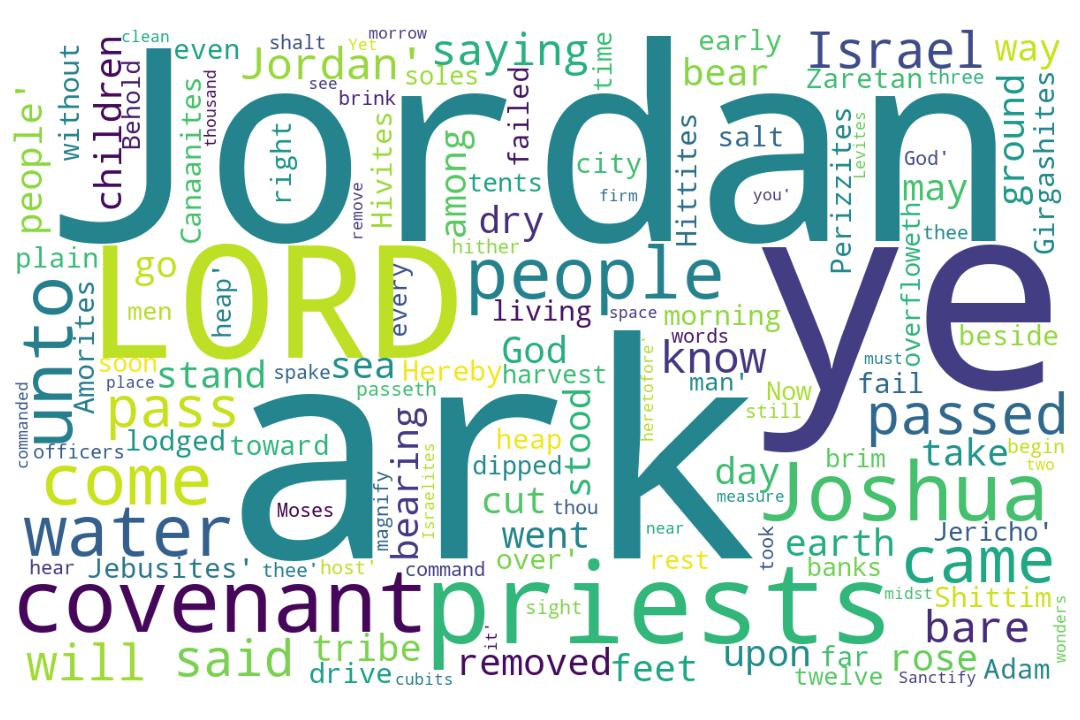
\includegraphics[width=\linewidth]{06OT-Joshua/Joshua3-WordCloud.jpg}
  \caption{Joshua 3 Word Cloud}
  \label{fig:Joshua 3 Word Cloud}
\end{figure}



\marginpar{\scriptsize \centering \fcolorbox{bone}{lime}{\textbf{CROSSING OVER}}\\ (Joshua 3:1-17) \begin{compactenum}[I.][8]
    \item A 3-Day \textbf{Wait} \index[scripture]{Joshua!Jsh 03:03}(Jsh 3:2) 
    \item The \textbf{Way} \index[scripture]{Joshua!Jsh 03:04}(Jsh 3:4) -- had to be miraculous
    \item \textbf{Wonders} Ahead \index[scripture]{Joshua!Jsh 03:05}(Jsh 3:5) 
    \item A Promise  \textbf{Without} Fail \index[scripture]{Joshua!Jsh 03:10}(Jsh 3:10) 
    \item The  \textbf{Waters}  \index[scripture]{Joshua!Jsh 03:13}  \index[scripture]{Joshua!Jsh 03:16} (Jsh 3:13, 16) 
    \item The  \textbf{Words} that Describe this  \index[scripture]{Joshua!Jsh 03:13}  \index[scripture]{Joshua!Jsh 03:16} (Jsh 3:13, 16) -- phrases include ``came over'' (4:22), ``carry over'' (4:3), ``carried over'' (4:8), ``pass over'' (3:6, 14, 4:5), ``passed over'' (3:1, 16, 17 -- 2x, 4:1, 4:7, 4:10, 4:11 -- 2x, 4:12, 4:13, 4:23, 5:1),.
   \item The  \textbf{Witnesses}  \index[scripture]{Joshua!Jsh 04:03}   (Jsh 4:3) 
\end{compactenum}}


\footnote{\textcolor[cmyk]{0.99998,1,0,0}{\hyperlink{TOC}{Return to end of Table of Contents.}}}\footnote{\href{https://audiobible.com/bible/joshua_1.html}{\textcolor[cmyk]{0.99998,1,0,0}{Joshua Audio}}}\textcolor[cmyk]{0.99998,1,0,0}{And Joshua rose early in the morning; and they removed from Shittim, and came to Jordan, he and all the children of Israel, and lodged there before they passed over.}
[2] \textcolor[cmyk]{0.99998,1,0,0}{And it came to pass after \fcolorbox{bone}{lime}{three days}, \fcolorbox{bone}{bone}{that} the officers went through the host;}
[3] \textcolor[cmyk]{0.99998,1,0,0}{And they commanded the people, saying, When ye see the ark of the covenant of the LORD your God, and the priests the Levites bearing it, then ye shall remove from your place, and go after it.}
[4] \textcolor[cmyk]{0.99998,1,0,0}{Yet there shall be a space between you and it, about two thousand cubits by measure: come not near unto it, \fcolorbox{bone}{bone}{that} ye may know the \fcolorbox{bone}{lime}{way} by which ye must go: for ye have not passed \emph{this} way heretofore.}
[5] \textcolor[cmyk]{0.99998,1,0,0}{And Joshua said unto the people, Sanctify yourselves: for to morrow the LORD will do \fcolorbox{bone}{lime}{wonders} among you.}
[6] \textcolor[cmyk]{0.99998,1,0,0}{And Joshua spake unto the priests, saying, Take up the ark of the covenant, and pass over before the people. And they took up the ark of the covenant, and went before the people.}\\
\\
\P \textcolor[cmyk]{0.99998,1,0,0}{And the LORD said unto Joshua, This day will I begin to magnify thee in the sight of all Israel, \fcolorbox{bone}{bone}{that} they may know that, as I was with Moses, \emph{so} I will be with thee.}
[8] \textcolor[cmyk]{0.99998,1,0,0}{And thou shalt command the priests \fcolorbox{bone}{bone}{that} bear the ark of the covenant, saying, When ye are come to the brink of the water of Jordan, ye shall stand still in Jordan.}\\
\\
\P \textcolor[cmyk]{0.99998,1,0,0}{And Joshua said unto the children of Israel, Come hither, and hear the words of the LORD your God.}
[10] \textcolor[cmyk]{0.99998,1,0,0}{And Joshua said, Hereby ye shall know \fcolorbox{bone}{bone}{that} the living God \emph{is} among you, and \emph{that} he will \fcolorbox{bone}{lime}{without fail} drive out from before you the Canaanites, and the Hittites, and the Hivites, and the Perizzites, and the Girgashites, and the Amorites, and the Jebusites.}
[11] \textcolor[cmyk]{0.99998,1,0,0}{Behold, the ark of the covenant of the Lord of all the earth passeth over before you into Jordan.}
[12] \textcolor[cmyk]{0.99998,1,0,0}{Now therefore take you twelve men out of the tribes of Israel, out of every tribe a man.}
[13] \textcolor[cmyk]{0.99998,1,0,0}{And it shall come to pass, as soon as the soles of the feet of the priests \fcolorbox{bone}{bone}{that} bear the ark of the LORD, the Lord of all the earth, shall rest in the \fcolorbox{bone}{lime}{waters} of Jordan, \emph{that} the waters of Jordan shall be cut off \emph{from} the waters \fcolorbox{bone}{bone}{that} come down from above; and they shall stand upon an heap.}
[14] \textcolor[cmyk]{0.99998,1,0,0}{And it came to pass, when the people removed from their tents, to pass over Jordan, and the priests bearing the ark of the covenant before the people;}
[15] \textcolor[cmyk]{0.99998,1,0,0}{And as they \fcolorbox{bone}{bone}{that} bare the ark were come unto Jordan, and the feet of the priests \fcolorbox{bone}{bone}{that} bare the ark were dipped in the brim of the water, (for Jordan overfloweth all his banks all the time of harvest,)}
[16] \textcolor[cmyk]{0.99998,1,0,0}{That the \fcolorbox{bone}{lime}{waters} which came down from above stood \emph{and} rose up upon an heap very far from the city Adam, \fcolorbox{bone}{bone}{that} \emph{is} beside Zaretan: and those \fcolorbox{bone}{bone}{that} came down toward the sea of the plain, \emph{even} the salt sea, failed, \emph{and} were cut off: and the people passed over right against Jericho.}
[17] \textcolor[cmyk]{0.99998,1,0,0}{And the priests \fcolorbox{bone}{bone}{that} bare the ark of the covenant of the LORD stood firm on dry ground in the midst of Jordan, and all the Israelites passed over on dry ground, until all the people were passed clean over Jordan.}\footnote{But lift thou up thy rod, and stretch out thine hand over the sea, and divide it: and the children of Israel shall go on dry ground through the midst of the sea.}\footnote{\textbf{2 Kings 2:8} - And Elijah took his mantle, and wrapped it together, and smote the waters, and they were divided hither and thither, so that they two went over on dry ground.And Elijah took his mantle, and wrapped it together, and smote the waters, and they were divided hither and thither, so that they two went over on dry ground.}
\index[NWIV]{30!Joshua!Jos 3:1}\index[AWIP]{And!Joshua!Jos 3:1}\index[AWIP]{Joshua!Joshua!Jos 3:1}\index[AWIP]{rose!Joshua!Jos 3:1}\index[AWIP]{early!Joshua!Jos 3:1}\index[AWIP]{in!Joshua!Jos 3:1}\index[AWIP]{the!Joshua!Jos 3:1}\index[AWIP]{the!Joshua!Jos 3:1 (2)}\index[AWIP]{morning!Joshua!Jos 3:1}\index[AWIP]{and!Joshua!Jos 3:1}\index[AWIP]{and!Joshua!Jos 3:1 (2)}\index[AWIP]{and!Joshua!Jos 3:1 (3)}\index[AWIP]{and!Joshua!Jos 3:1 (4)}\index[AWIP]{they!Joshua!Jos 3:1}\index[AWIP]{they!Joshua!Jos 3:1 (2)}\index[AWIP]{removed!Joshua!Jos 3:1}\index[AWIP]{from!Joshua!Jos 3:1}\index[AWIP]{Shittim!Joshua!Jos 3:1}\index[AWIP]{came!Joshua!Jos 3:1}\index[AWIP]{to!Joshua!Jos 3:1}\index[AWIP]{Jordan!Joshua!Jos 3:1}\index[AWIP]{he!Joshua!Jos 3:1}\index[AWIP]{all!Joshua!Jos 3:1}\index[AWIP]{children!Joshua!Jos 3:1}\index[AWIP]{of!Joshua!Jos 3:1}\index[AWIP]{Israel!Joshua!Jos 3:1}\index[AWIP]{lodged!Joshua!Jos 3:1}\index[AWIP]{there!Joshua!Jos 3:1}\index[AWIP]{before!Joshua!Jos 3:1}\index[AWIP]{passed!Joshua!Jos 3:1}\index[AWIP]{over!Joshua!Jos 3:1}

\index[NWIV]{15!Joshua!Jos 3:2}\index[AWIP]{And!Joshua!Jos 3:2}\index[AWIP]{it!Joshua!Jos 3:2}\index[AWIP]{came!Joshua!Jos 3:2}\index[AWIP]{to!Joshua!Jos 3:2}\index[AWIP]{pass!Joshua!Jos 3:2}\index[AWIP]{after!Joshua!Jos 3:2}\index[AWIP]{three!Joshua!Jos 3:2}\index[AWIP]{days!Joshua!Jos 3:2}\index[AWIP]{that!Joshua!Jos 3:2}\index[AWIP]{the!Joshua!Jos 3:2}\index[AWIP]{the!Joshua!Jos 3:2 (2)}\index[AWIP]{officers!Joshua!Jos 3:2}\index[AWIP]{went!Joshua!Jos 3:2}\index[AWIP]{through!Joshua!Jos 3:2}\index[AWIP]{host!Joshua!Jos 3:2}

\index[NWIV]{37!Joshua!Jos 3:3}\index[AWIP]{And!Joshua!Jos 3:3}\index[AWIP]{they!Joshua!Jos 3:3}\index[AWIP]{commanded!Joshua!Jos 3:3}\index[AWIP]{the!Joshua!Jos 3:3}\index[AWIP]{the!Joshua!Jos 3:3 (2)}\index[AWIP]{the!Joshua!Jos 3:3 (3)}\index[AWIP]{the!Joshua!Jos 3:3 (4)}\index[AWIP]{the!Joshua!Jos 3:3 (5)}\index[AWIP]{the!Joshua!Jos 3:3 (6)}\index[AWIP]{people!Joshua!Jos 3:3}\index[AWIP]{saying!Joshua!Jos 3:3}\index[AWIP]{When!Joshua!Jos 3:3}\index[AWIP]{ye!Joshua!Jos 3:3}\index[AWIP]{ye!Joshua!Jos 3:3 (2)}\index[AWIP]{see!Joshua!Jos 3:3}\index[AWIP]{ark!Joshua!Jos 3:3}\index[AWIP]{of!Joshua!Jos 3:3}\index[AWIP]{of!Joshua!Jos 3:3 (2)}\index[AWIP]{covenant!Joshua!Jos 3:3}\index[AWIP]{LORD!Joshua!Jos 3:3}\index[AWIP]{your!Joshua!Jos 3:3}\index[AWIP]{your!Joshua!Jos 3:3 (2)}\index[AWIP]{God!Joshua!Jos 3:3}\index[AWIP]{and!Joshua!Jos 3:3}\index[AWIP]{and!Joshua!Jos 3:3 (2)}\index[AWIP]{priests!Joshua!Jos 3:3}\index[AWIP]{Levites!Joshua!Jos 3:3}\index[AWIP]{bearing!Joshua!Jos 3:3}\index[AWIP]{it!Joshua!Jos 3:3}\index[AWIP]{it!Joshua!Jos 3:3 (2)}\index[AWIP]{then!Joshua!Jos 3:3}\index[AWIP]{shall!Joshua!Jos 3:3}\index[AWIP]{remove!Joshua!Jos 3:3}\index[AWIP]{from!Joshua!Jos 3:3}\index[AWIP]{place!Joshua!Jos 3:3}\index[AWIP]{go!Joshua!Jos 3:3}\index[AWIP]{after!Joshua!Jos 3:3}

\index[NWIV]{40!Joshua!Jos 3:4}\index[AWIP]{Yet!Joshua!Jos 3:4}\index[AWIP]{there!Joshua!Jos 3:4}\index[AWIP]{shall!Joshua!Jos 3:4}\index[AWIP]{be!Joshua!Jos 3:4}\index[AWIP]{a!Joshua!Jos 3:4}\index[AWIP]{space!Joshua!Jos 3:4}\index[AWIP]{between!Joshua!Jos 3:4}\index[AWIP]{you!Joshua!Jos 3:4}\index[AWIP]{and!Joshua!Jos 3:4}\index[AWIP]{it!Joshua!Jos 3:4}\index[AWIP]{it!Joshua!Jos 3:4 (2)}\index[AWIP]{about!Joshua!Jos 3:4}\index[AWIP]{two!Joshua!Jos 3:4}\index[AWIP]{thousand!Joshua!Jos 3:4}\index[AWIP]{cubits!Joshua!Jos 3:4}\index[AWIP]{by!Joshua!Jos 3:4}\index[AWIP]{by!Joshua!Jos 3:4 (2)}\index[AWIP]{measure!Joshua!Jos 3:4}\index[AWIP]{come!Joshua!Jos 3:4}\index[AWIP]{not!Joshua!Jos 3:4}\index[AWIP]{not!Joshua!Jos 3:4 (2)}\index[AWIP]{near!Joshua!Jos 3:4}\index[AWIP]{unto!Joshua!Jos 3:4}\index[AWIP]{that!Joshua!Jos 3:4}\index[AWIP]{ye!Joshua!Jos 3:4}\index[AWIP]{ye!Joshua!Jos 3:4 (2)}\index[AWIP]{ye!Joshua!Jos 3:4 (3)}\index[AWIP]{may!Joshua!Jos 3:4}\index[AWIP]{know!Joshua!Jos 3:4}\index[AWIP]{the!Joshua!Jos 3:4}\index[AWIP]{way!Joshua!Jos 3:4}\index[AWIP]{way!Joshua!Jos 3:4 (2)}\index[AWIP]{which!Joshua!Jos 3:4}\index[AWIP]{must!Joshua!Jos 3:4}\index[AWIP]{go!Joshua!Jos 3:4}\index[AWIP]{for!Joshua!Jos 3:4}\index[AWIP]{have!Joshua!Jos 3:4}\index[AWIP]{passed!Joshua!Jos 3:4}\index[AWIP]{\emph{this}!Joshua!Jos 3:4}\index[AWIP]{heretofore!Joshua!Jos 3:4}\index[AWIP]{\emph{this}!Joshua!Jos 3:4}

\index[NWIV]{18!Joshua!Jos 3:5}\index[AWIP]{And!Joshua!Jos 3:5}\index[AWIP]{Joshua!Joshua!Jos 3:5}\index[AWIP]{said!Joshua!Jos 3:5}\index[AWIP]{unto!Joshua!Jos 3:5}\index[AWIP]{the!Joshua!Jos 3:5}\index[AWIP]{the!Joshua!Jos 3:5 (2)}\index[AWIP]{people!Joshua!Jos 3:5}\index[AWIP]{Sanctify!Joshua!Jos 3:5}\index[AWIP]{yourselves!Joshua!Jos 3:5}\index[AWIP]{for!Joshua!Jos 3:5}\index[AWIP]{to!Joshua!Jos 3:5}\index[AWIP]{morrow!Joshua!Jos 3:5}\index[AWIP]{LORD!Joshua!Jos 3:5}\index[AWIP]{will!Joshua!Jos 3:5}\index[AWIP]{do!Joshua!Jos 3:5}\index[AWIP]{wonders!Joshua!Jos 3:5}\index[AWIP]{among!Joshua!Jos 3:5}\index[AWIP]{you!Joshua!Jos 3:5}

\index[NWIV]{34!Joshua!Jos 3:6}\index[AWIP]{And!Joshua!Jos 3:6}\index[AWIP]{And!Joshua!Jos 3:6 (2)}\index[AWIP]{Joshua!Joshua!Jos 3:6}\index[AWIP]{spake!Joshua!Jos 3:6}\index[AWIP]{unto!Joshua!Jos 3:6}\index[AWIP]{the!Joshua!Jos 3:6}\index[AWIP]{the!Joshua!Jos 3:6 (2)}\index[AWIP]{the!Joshua!Jos 3:6 (3)}\index[AWIP]{the!Joshua!Jos 3:6 (4)}\index[AWIP]{the!Joshua!Jos 3:6 (5)}\index[AWIP]{the!Joshua!Jos 3:6 (6)}\index[AWIP]{the!Joshua!Jos 3:6 (7)}\index[AWIP]{priests!Joshua!Jos 3:6}\index[AWIP]{saying!Joshua!Jos 3:6}\index[AWIP]{Take!Joshua!Jos 3:6}\index[AWIP]{up!Joshua!Jos 3:6}\index[AWIP]{up!Joshua!Jos 3:6 (2)}\index[AWIP]{ark!Joshua!Jos 3:6}\index[AWIP]{ark!Joshua!Jos 3:6 (2)}\index[AWIP]{of!Joshua!Jos 3:6}\index[AWIP]{of!Joshua!Jos 3:6 (2)}\index[AWIP]{covenant!Joshua!Jos 3:6}\index[AWIP]{covenant!Joshua!Jos 3:6 (2)}\index[AWIP]{and!Joshua!Jos 3:6}\index[AWIP]{and!Joshua!Jos 3:6 (2)}\index[AWIP]{pass!Joshua!Jos 3:6}\index[AWIP]{over!Joshua!Jos 3:6}\index[AWIP]{before!Joshua!Jos 3:6}\index[AWIP]{before!Joshua!Jos 3:6 (2)}\index[AWIP]{people!Joshua!Jos 3:6}\index[AWIP]{people!Joshua!Jos 3:6 (2)}\index[AWIP]{they!Joshua!Jos 3:6}\index[AWIP]{took!Joshua!Jos 3:6}\index[AWIP]{went!Joshua!Jos 3:6}

\index[NWIV]{36!Joshua!Jos 3:7}\index[AWIP]{And!Joshua!Jos 3:7}\index[AWIP]{the!Joshua!Jos 3:7}\index[AWIP]{the!Joshua!Jos 3:7 (2)}\index[AWIP]{LORD!Joshua!Jos 3:7}\index[AWIP]{said!Joshua!Jos 3:7}\index[AWIP]{unto!Joshua!Jos 3:7}\index[AWIP]{Joshua!Joshua!Jos 3:7}\index[AWIP]{This!Joshua!Jos 3:7}\index[AWIP]{day!Joshua!Jos 3:7}\index[AWIP]{will!Joshua!Jos 3:7}\index[AWIP]{will!Joshua!Jos 3:7 (2)}\index[AWIP]{I!Joshua!Jos 3:7}\index[AWIP]{I!Joshua!Jos 3:7 (2)}\index[AWIP]{I!Joshua!Jos 3:7 (3)}\index[AWIP]{begin!Joshua!Jos 3:7}\index[AWIP]{to!Joshua!Jos 3:7}\index[AWIP]{magnify!Joshua!Jos 3:7}\index[AWIP]{thee!Joshua!Jos 3:7}\index[AWIP]{thee!Joshua!Jos 3:7 (2)}\index[AWIP]{in!Joshua!Jos 3:7}\index[AWIP]{sight!Joshua!Jos 3:7}\index[AWIP]{of!Joshua!Jos 3:7}\index[AWIP]{all!Joshua!Jos 3:7}\index[AWIP]{Israel!Joshua!Jos 3:7}\index[AWIP]{that!Joshua!Jos 3:7}\index[AWIP]{that!Joshua!Jos 3:7 (2)}\index[AWIP]{they!Joshua!Jos 3:7}\index[AWIP]{may!Joshua!Jos 3:7}\index[AWIP]{know!Joshua!Jos 3:7}\index[AWIP]{as!Joshua!Jos 3:7}\index[AWIP]{was!Joshua!Jos 3:7}\index[AWIP]{with!Joshua!Jos 3:7}\index[AWIP]{with!Joshua!Jos 3:7 (2)}\index[AWIP]{Moses!Joshua!Jos 3:7}\index[AWIP]{\emph{so}!Joshua!Jos 3:7}\index[AWIP]{be!Joshua!Jos 3:7}\index[AWIP]{\emph{so}!Joshua!Jos 3:7}

\index[NWIV]{32!Joshua!Jos 3:8}\index[AWIP]{And!Joshua!Jos 3:8}\index[AWIP]{thou!Joshua!Jos 3:8}\index[AWIP]{shalt!Joshua!Jos 3:8}\index[AWIP]{command!Joshua!Jos 3:8}\index[AWIP]{the!Joshua!Jos 3:8}\index[AWIP]{the!Joshua!Jos 3:8 (2)}\index[AWIP]{the!Joshua!Jos 3:8 (3)}\index[AWIP]{the!Joshua!Jos 3:8 (4)}\index[AWIP]{the!Joshua!Jos 3:8 (5)}\index[AWIP]{priests!Joshua!Jos 3:8}\index[AWIP]{that!Joshua!Jos 3:8}\index[AWIP]{bear!Joshua!Jos 3:8}\index[AWIP]{ark!Joshua!Jos 3:8}\index[AWIP]{of!Joshua!Jos 3:8}\index[AWIP]{of!Joshua!Jos 3:8 (2)}\index[AWIP]{of!Joshua!Jos 3:8 (3)}\index[AWIP]{covenant!Joshua!Jos 3:8}\index[AWIP]{saying!Joshua!Jos 3:8}\index[AWIP]{When!Joshua!Jos 3:8}\index[AWIP]{ye!Joshua!Jos 3:8}\index[AWIP]{ye!Joshua!Jos 3:8 (2)}\index[AWIP]{are!Joshua!Jos 3:8}\index[AWIP]{come!Joshua!Jos 3:8}\index[AWIP]{to!Joshua!Jos 3:8}\index[AWIP]{brink!Joshua!Jos 3:8}\index[AWIP]{water!Joshua!Jos 3:8}\index[AWIP]{Jordan!Joshua!Jos 3:8}\index[AWIP]{Jordan!Joshua!Jos 3:8 (2)}\index[AWIP]{shall!Joshua!Jos 3:8}\index[AWIP]{stand!Joshua!Jos 3:8}\index[AWIP]{still!Joshua!Jos 3:8}\index[AWIP]{in!Joshua!Jos 3:8}

\index[NWIV]{19!Joshua!Jos 3:9}\index[AWIP]{And!Joshua!Jos 3:9}\index[AWIP]{Joshua!Joshua!Jos 3:9}\index[AWIP]{said!Joshua!Jos 3:9}\index[AWIP]{unto!Joshua!Jos 3:9}\index[AWIP]{the!Joshua!Jos 3:9}\index[AWIP]{the!Joshua!Jos 3:9 (2)}\index[AWIP]{the!Joshua!Jos 3:9 (3)}\index[AWIP]{children!Joshua!Jos 3:9}\index[AWIP]{of!Joshua!Jos 3:9}\index[AWIP]{of!Joshua!Jos 3:9 (2)}\index[AWIP]{Israel!Joshua!Jos 3:9}\index[AWIP]{Come!Joshua!Jos 3:9}\index[AWIP]{hither!Joshua!Jos 3:9}\index[AWIP]{and!Joshua!Jos 3:9}\index[AWIP]{hear!Joshua!Jos 3:9}\index[AWIP]{words!Joshua!Jos 3:9}\index[AWIP]{LORD!Joshua!Jos 3:9}\index[AWIP]{your!Joshua!Jos 3:9}\index[AWIP]{God!Joshua!Jos 3:9}

\index[NWIV]{45!Joshua!Jos 3:10}\index[AWIP]{And!Joshua!Jos 3:10}\index[AWIP]{Joshua!Joshua!Jos 3:10}\index[AWIP]{said!Joshua!Jos 3:10}\index[AWIP]{Hereby!Joshua!Jos 3:10}\index[AWIP]{ye!Joshua!Jos 3:10}\index[AWIP]{shall!Joshua!Jos 3:10}\index[AWIP]{know!Joshua!Jos 3:10}\index[AWIP]{that!Joshua!Jos 3:10}\index[AWIP]{the!Joshua!Jos 3:10}\index[AWIP]{the!Joshua!Jos 3:10 (2)}\index[AWIP]{the!Joshua!Jos 3:10 (3)}\index[AWIP]{the!Joshua!Jos 3:10 (4)}\index[AWIP]{the!Joshua!Jos 3:10 (5)}\index[AWIP]{the!Joshua!Jos 3:10 (6)}\index[AWIP]{the!Joshua!Jos 3:10 (7)}\index[AWIP]{the!Joshua!Jos 3:10 (8)}\index[AWIP]{living!Joshua!Jos 3:10}\index[AWIP]{God!Joshua!Jos 3:10}\index[AWIP]{\emph{is}!Joshua!Jos 3:10}\index[AWIP]{among!Joshua!Jos 3:10}\index[AWIP]{you!Joshua!Jos 3:10}\index[AWIP]{you!Joshua!Jos 3:10 (2)}\index[AWIP]{and!Joshua!Jos 3:10}\index[AWIP]{and!Joshua!Jos 3:10 (2)}\index[AWIP]{and!Joshua!Jos 3:10 (3)}\index[AWIP]{and!Joshua!Jos 3:10 (4)}\index[AWIP]{and!Joshua!Jos 3:10 (5)}\index[AWIP]{and!Joshua!Jos 3:10 (6)}\index[AWIP]{and!Joshua!Jos 3:10 (7)}\index[AWIP]{\emph{that}!Joshua!Jos 3:10}\index[AWIP]{he!Joshua!Jos 3:10}\index[AWIP]{will!Joshua!Jos 3:10}\index[AWIP]{without!Joshua!Jos 3:10}\index[AWIP]{fail!Joshua!Jos 3:10}\index[AWIP]{drive!Joshua!Jos 3:10}\index[AWIP]{out!Joshua!Jos 3:10}\index[AWIP]{from!Joshua!Jos 3:10}\index[AWIP]{before!Joshua!Jos 3:10}\index[AWIP]{Canaanites!Joshua!Jos 3:10}\index[AWIP]{Hittites!Joshua!Jos 3:10}\index[AWIP]{Hivites!Joshua!Jos 3:10}\index[AWIP]{Perizzites!Joshua!Jos 3:10}\index[AWIP]{Girgashites!Joshua!Jos 3:10}\index[AWIP]{Amorites!Joshua!Jos 3:10}\index[AWIP]{Jebusites!Joshua!Jos 3:10}\index[AWIP]{\emph{is}!Joshua!Jos 3:10}\index[AWIP]{\emph{that}!Joshua!Jos 3:10}

\index[NWIV]{19!Joshua!Jos 3:11}\index[AWIP]{Behold!Joshua!Jos 3:11}\index[AWIP]{the!Joshua!Jos 3:11}\index[AWIP]{the!Joshua!Jos 3:11 (2)}\index[AWIP]{the!Joshua!Jos 3:11 (3)}\index[AWIP]{the!Joshua!Jos 3:11 (4)}\index[AWIP]{ark!Joshua!Jos 3:11}\index[AWIP]{of!Joshua!Jos 3:11}\index[AWIP]{of!Joshua!Jos 3:11 (2)}\index[AWIP]{of!Joshua!Jos 3:11 (3)}\index[AWIP]{covenant!Joshua!Jos 3:11}\index[AWIP]{Lord!Joshua!Jos 3:11}\index[AWIP]{all!Joshua!Jos 3:11}\index[AWIP]{earth!Joshua!Jos 3:11}\index[AWIP]{passeth!Joshua!Jos 3:11}\index[AWIP]{over!Joshua!Jos 3:11}\index[AWIP]{before!Joshua!Jos 3:11}\index[AWIP]{you!Joshua!Jos 3:11}\index[AWIP]{into!Joshua!Jos 3:11}\index[AWIP]{Jordan!Joshua!Jos 3:11}

\index[NWIV]{18!Joshua!Jos 3:12}\index[AWIP]{Now!Joshua!Jos 3:12}\index[AWIP]{therefore!Joshua!Jos 3:12}\index[AWIP]{take!Joshua!Jos 3:12}\index[AWIP]{you!Joshua!Jos 3:12}\index[AWIP]{twelve!Joshua!Jos 3:12}\index[AWIP]{men!Joshua!Jos 3:12}\index[AWIP]{out!Joshua!Jos 3:12}\index[AWIP]{out!Joshua!Jos 3:12 (2)}\index[AWIP]{of!Joshua!Jos 3:12}\index[AWIP]{of!Joshua!Jos 3:12 (2)}\index[AWIP]{of!Joshua!Jos 3:12 (3)}\index[AWIP]{the!Joshua!Jos 3:12}\index[AWIP]{tribes!Joshua!Jos 3:12}\index[AWIP]{Israel!Joshua!Jos 3:12}\index[AWIP]{every!Joshua!Jos 3:12}\index[AWIP]{tribe!Joshua!Jos 3:12}\index[AWIP]{a!Joshua!Jos 3:12}\index[AWIP]{man!Joshua!Jos 3:12}

\index[NWIV]{61!Joshua!Jos 3:13}\index[AWIP]{And!Joshua!Jos 3:13}\index[AWIP]{it!Joshua!Jos 3:13}\index[AWIP]{shall!Joshua!Jos 3:13}\index[AWIP]{shall!Joshua!Jos 3:13 (2)}\index[AWIP]{shall!Joshua!Jos 3:13 (3)}\index[AWIP]{shall!Joshua!Jos 3:13 (4)}\index[AWIP]{come!Joshua!Jos 3:13}\index[AWIP]{come!Joshua!Jos 3:13 (2)}\index[AWIP]{to!Joshua!Jos 3:13}\index[AWIP]{pass!Joshua!Jos 3:13}\index[AWIP]{as!Joshua!Jos 3:13}\index[AWIP]{as!Joshua!Jos 3:13 (2)}\index[AWIP]{soon!Joshua!Jos 3:13}\index[AWIP]{the!Joshua!Jos 3:13}\index[AWIP]{the!Joshua!Jos 3:13 (2)}\index[AWIP]{the!Joshua!Jos 3:13 (3)}\index[AWIP]{the!Joshua!Jos 3:13 (4)}\index[AWIP]{the!Joshua!Jos 3:13 (5)}\index[AWIP]{the!Joshua!Jos 3:13 (6)}\index[AWIP]{the!Joshua!Jos 3:13 (7)}\index[AWIP]{the!Joshua!Jos 3:13 (8)}\index[AWIP]{the!Joshua!Jos 3:13 (9)}\index[AWIP]{the!Joshua!Jos 3:13 (10)}\index[AWIP]{soles!Joshua!Jos 3:13}\index[AWIP]{of!Joshua!Jos 3:13}\index[AWIP]{of!Joshua!Jos 3:13 (2)}\index[AWIP]{of!Joshua!Jos 3:13 (3)}\index[AWIP]{of!Joshua!Jos 3:13 (4)}\index[AWIP]{of!Joshua!Jos 3:13 (5)}\index[AWIP]{of!Joshua!Jos 3:13 (6)}\index[AWIP]{feet!Joshua!Jos 3:13}\index[AWIP]{priests!Joshua!Jos 3:13}\index[AWIP]{that!Joshua!Jos 3:13}\index[AWIP]{that!Joshua!Jos 3:13 (2)}\index[AWIP]{bear!Joshua!Jos 3:13}\index[AWIP]{ark!Joshua!Jos 3:13}\index[AWIP]{LORD!Joshua!Jos 3:13}\index[AWIP]{Lord!Joshua!Jos 3:13}\index[AWIP]{all!Joshua!Jos 3:13}\index[AWIP]{earth!Joshua!Jos 3:13}\index[AWIP]{rest!Joshua!Jos 3:13}\index[AWIP]{in!Joshua!Jos 3:13}\index[AWIP]{waters!Joshua!Jos 3:13}\index[AWIP]{waters!Joshua!Jos 3:13 (2)}\index[AWIP]{waters!Joshua!Jos 3:13 (3)}\index[AWIP]{Jordan!Joshua!Jos 3:13}\index[AWIP]{Jordan!Joshua!Jos 3:13 (2)}\index[AWIP]{\emph{that}!Joshua!Jos 3:13}\index[AWIP]{be!Joshua!Jos 3:13}\index[AWIP]{cut!Joshua!Jos 3:13}\index[AWIP]{off!Joshua!Jos 3:13}\index[AWIP]{\emph{from}!Joshua!Jos 3:13}\index[AWIP]{down!Joshua!Jos 3:13}\index[AWIP]{from!Joshua!Jos 3:13}\index[AWIP]{above!Joshua!Jos 3:13}\index[AWIP]{and!Joshua!Jos 3:13}\index[AWIP]{they!Joshua!Jos 3:13}\index[AWIP]{stand!Joshua!Jos 3:13}\index[AWIP]{upon!Joshua!Jos 3:13}\index[AWIP]{an!Joshua!Jos 3:13}\index[AWIP]{heap!Joshua!Jos 3:13}\index[AWIP]{\emph{that}!Joshua!Jos 3:13}\index[AWIP]{\emph{from}!Joshua!Jos 3:13}

\index[NWIV]{28!Joshua!Jos 3:14}\index[AWIP]{And!Joshua!Jos 3:14}\index[AWIP]{it!Joshua!Jos 3:14}\index[AWIP]{came!Joshua!Jos 3:14}\index[AWIP]{to!Joshua!Jos 3:14}\index[AWIP]{to!Joshua!Jos 3:14 (2)}\index[AWIP]{pass!Joshua!Jos 3:14}\index[AWIP]{pass!Joshua!Jos 3:14 (2)}\index[AWIP]{when!Joshua!Jos 3:14}\index[AWIP]{the!Joshua!Jos 3:14}\index[AWIP]{the!Joshua!Jos 3:14 (2)}\index[AWIP]{the!Joshua!Jos 3:14 (3)}\index[AWIP]{the!Joshua!Jos 3:14 (4)}\index[AWIP]{the!Joshua!Jos 3:14 (5)}\index[AWIP]{people!Joshua!Jos 3:14}\index[AWIP]{people!Joshua!Jos 3:14 (2)}\index[AWIP]{removed!Joshua!Jos 3:14}\index[AWIP]{from!Joshua!Jos 3:14}\index[AWIP]{their!Joshua!Jos 3:14}\index[AWIP]{tents!Joshua!Jos 3:14}\index[AWIP]{over!Joshua!Jos 3:14}\index[AWIP]{Jordan!Joshua!Jos 3:14}\index[AWIP]{and!Joshua!Jos 3:14}\index[AWIP]{priests!Joshua!Jos 3:14}\index[AWIP]{bearing!Joshua!Jos 3:14}\index[AWIP]{ark!Joshua!Jos 3:14}\index[AWIP]{of!Joshua!Jos 3:14}\index[AWIP]{covenant!Joshua!Jos 3:14}\index[AWIP]{before!Joshua!Jos 3:14}

\index[NWIV]{40!Joshua!Jos 3:15}\index[AWIP]{And!Joshua!Jos 3:15}\index[AWIP]{as!Joshua!Jos 3:15}\index[AWIP]{they!Joshua!Jos 3:15}\index[AWIP]{that!Joshua!Jos 3:15}\index[AWIP]{that!Joshua!Jos 3:15 (2)}\index[AWIP]{bare!Joshua!Jos 3:15}\index[AWIP]{bare!Joshua!Jos 3:15 (2)}\index[AWIP]{the!Joshua!Jos 3:15}\index[AWIP]{the!Joshua!Jos 3:15 (2)}\index[AWIP]{the!Joshua!Jos 3:15 (3)}\index[AWIP]{the!Joshua!Jos 3:15 (4)}\index[AWIP]{the!Joshua!Jos 3:15 (5)}\index[AWIP]{the!Joshua!Jos 3:15 (6)}\index[AWIP]{the!Joshua!Jos 3:15 (7)}\index[AWIP]{ark!Joshua!Jos 3:15}\index[AWIP]{ark!Joshua!Jos 3:15 (2)}\index[AWIP]{were!Joshua!Jos 3:15}\index[AWIP]{were!Joshua!Jos 3:15 (2)}\index[AWIP]{come!Joshua!Jos 3:15}\index[AWIP]{unto!Joshua!Jos 3:15}\index[AWIP]{Jordan!Joshua!Jos 3:15}\index[AWIP]{Jordan!Joshua!Jos 3:15 (2)}\index[AWIP]{and!Joshua!Jos 3:15}\index[AWIP]{feet!Joshua!Jos 3:15}\index[AWIP]{of!Joshua!Jos 3:15}\index[AWIP]{of!Joshua!Jos 3:15 (2)}\index[AWIP]{of!Joshua!Jos 3:15 (3)}\index[AWIP]{priests!Joshua!Jos 3:15}\index[AWIP]{dipped!Joshua!Jos 3:15}\index[AWIP]{in!Joshua!Jos 3:15}\index[AWIP]{brim!Joshua!Jos 3:15}\index[AWIP]{water!Joshua!Jos 3:15}\index[AWIP]{(for!Joshua!Jos 3:15}\index[AWIP]{overfloweth!Joshua!Jos 3:15}\index[AWIP]{all!Joshua!Jos 3:15}\index[AWIP]{all!Joshua!Jos 3:15 (2)}\index[AWIP]{his!Joshua!Jos 3:15}\index[AWIP]{banks!Joshua!Jos 3:15}\index[AWIP]{time!Joshua!Jos 3:15}\index[AWIP]{harvest)!Joshua!Jos 3:15}

\index[NWIV]{53!Joshua!Jos 3:16}\index[AWIP]{That!Joshua!Jos 3:16}\index[AWIP]{the!Joshua!Jos 3:16}\index[AWIP]{the!Joshua!Jos 3:16 (2)}\index[AWIP]{the!Joshua!Jos 3:16 (3)}\index[AWIP]{the!Joshua!Jos 3:16 (4)}\index[AWIP]{the!Joshua!Jos 3:16 (5)}\index[AWIP]{the!Joshua!Jos 3:16 (6)}\index[AWIP]{waters!Joshua!Jos 3:16}\index[AWIP]{which!Joshua!Jos 3:16}\index[AWIP]{came!Joshua!Jos 3:16}\index[AWIP]{came!Joshua!Jos 3:16 (2)}\index[AWIP]{down!Joshua!Jos 3:16}\index[AWIP]{down!Joshua!Jos 3:16 (2)}\index[AWIP]{from!Joshua!Jos 3:16}\index[AWIP]{from!Joshua!Jos 3:16 (2)}\index[AWIP]{above!Joshua!Jos 3:16}\index[AWIP]{stood!Joshua!Jos 3:16}\index[AWIP]{\emph{and}!Joshua!Jos 3:16}\index[AWIP]{\emph{and}!Joshua!Jos 3:16 (2)}\index[AWIP]{rose!Joshua!Jos 3:16}\index[AWIP]{up!Joshua!Jos 3:16}\index[AWIP]{upon!Joshua!Jos 3:16}\index[AWIP]{an!Joshua!Jos 3:16}\index[AWIP]{heap!Joshua!Jos 3:16}\index[AWIP]{very!Joshua!Jos 3:16}\index[AWIP]{far!Joshua!Jos 3:16}\index[AWIP]{city!Joshua!Jos 3:16}\index[AWIP]{Adam!Joshua!Jos 3:16}\index[AWIP]{that!Joshua!Jos 3:16}\index[AWIP]{that!Joshua!Jos 3:16 (2)}\index[AWIP]{\emph{is}!Joshua!Jos 3:16}\index[AWIP]{beside!Joshua!Jos 3:16}\index[AWIP]{Zaretan!Joshua!Jos 3:16}\index[AWIP]{and!Joshua!Jos 3:16}\index[AWIP]{and!Joshua!Jos 3:16 (2)}\index[AWIP]{those!Joshua!Jos 3:16}\index[AWIP]{toward!Joshua!Jos 3:16}\index[AWIP]{sea!Joshua!Jos 3:16}\index[AWIP]{sea!Joshua!Jos 3:16 (2)}\index[AWIP]{of!Joshua!Jos 3:16}\index[AWIP]{plain!Joshua!Jos 3:16}\index[AWIP]{\emph{even}!Joshua!Jos 3:16}\index[AWIP]{salt!Joshua!Jos 3:16}\index[AWIP]{failed!Joshua!Jos 3:16}\index[AWIP]{were!Joshua!Jos 3:16}\index[AWIP]{cut!Joshua!Jos 3:16}\index[AWIP]{off!Joshua!Jos 3:16}\index[AWIP]{people!Joshua!Jos 3:16}\index[AWIP]{passed!Joshua!Jos 3:16}\index[AWIP]{over!Joshua!Jos 3:16}\index[AWIP]{right!Joshua!Jos 3:16}\index[AWIP]{against!Joshua!Jos 3:16}\index[AWIP]{Jericho!Joshua!Jos 3:16}\index[AWIP]{\emph{and}!Joshua!Jos 3:16}\index[AWIP]{\emph{and}!Joshua!Jos 3:16 (2)}\index[AWIP]{\emph{is}!Joshua!Jos 3:16}\index[AWIP]{\emph{even}!Joshua!Jos 3:16}

\index[NWIV]{41!Joshua!Jos 3:17}\index[AWIP]{And!Joshua!Jos 3:17}\index[AWIP]{the!Joshua!Jos 3:17}\index[AWIP]{the!Joshua!Jos 3:17 (2)}\index[AWIP]{the!Joshua!Jos 3:17 (3)}\index[AWIP]{the!Joshua!Jos 3:17 (4)}\index[AWIP]{the!Joshua!Jos 3:17 (5)}\index[AWIP]{the!Joshua!Jos 3:17 (6)}\index[AWIP]{the!Joshua!Jos 3:17 (7)}\index[AWIP]{priests!Joshua!Jos 3:17}\index[AWIP]{that!Joshua!Jos 3:17}\index[AWIP]{bare!Joshua!Jos 3:17}\index[AWIP]{ark!Joshua!Jos 3:17}\index[AWIP]{of!Joshua!Jos 3:17}\index[AWIP]{of!Joshua!Jos 3:17 (2)}\index[AWIP]{of!Joshua!Jos 3:17 (3)}\index[AWIP]{covenant!Joshua!Jos 3:17}\index[AWIP]{LORD!Joshua!Jos 3:17}\index[AWIP]{stood!Joshua!Jos 3:17}\index[AWIP]{firm!Joshua!Jos 3:17}\index[AWIP]{on!Joshua!Jos 3:17}\index[AWIP]{on!Joshua!Jos 3:17 (2)}\index[AWIP]{dry!Joshua!Jos 3:17}\index[AWIP]{dry!Joshua!Jos 3:17 (2)}\index[AWIP]{ground!Joshua!Jos 3:17}\index[AWIP]{ground!Joshua!Jos 3:17 (2)}\index[AWIP]{in!Joshua!Jos 3:17}\index[AWIP]{midst!Joshua!Jos 3:17}\index[AWIP]{Jordan!Joshua!Jos 3:17}\index[AWIP]{Jordan!Joshua!Jos 3:17 (2)}\index[AWIP]{and!Joshua!Jos 3:17}\index[AWIP]{all!Joshua!Jos 3:17}\index[AWIP]{all!Joshua!Jos 3:17 (2)}\index[AWIP]{Israelites!Joshua!Jos 3:17}\index[AWIP]{passed!Joshua!Jos 3:17}\index[AWIP]{passed!Joshua!Jos 3:17 (2)}\index[AWIP]{over!Joshua!Jos 3:17}\index[AWIP]{over!Joshua!Jos 3:17 (2)}\index[AWIP]{until!Joshua!Jos 3:17}\index[AWIP]{people!Joshua!Jos 3:17}\index[AWIP]{were!Joshua!Jos 3:17}\index[AWIP]{clean!Joshua!Jos 3:17}


\section{Joshua 3 Outlines}

\subsection{My Outlines}

\subsubsection{Crossing Over}
\index[speaker]{Keith Anthony!Joshua 03 (Crossing Over)}
\index[series]{Joshua (Keith Anthony)!Joshua 03 (Crossing Over)}
\index[date]{2018/03/05!Joshua 03 (Crossing Over) (Keith Anthony)}
\begin{compactenum}[I.]
    \item A 3-Day \textbf{Wait} \index[scripture]{Joshua!Jsh 03:03}(Jsh 3:2) 
    \item The \textbf{Way} \index[scripture]{Joshua!Jsh 03:04}(Jsh 3:4) -- had to be miraculous
    \item \textbf{Wonders} Ahead \index[scripture]{Joshua!Jsh 03:05}(Jsh 3:5) 
    \item A Promise  \textbf{Without} Fail \index[scripture]{Joshua!Jsh 03:10}(Jsh 3:10) 
    \item The  \textbf{Waters}  \index[scripture]{Joshua!Jsh 03:13}  \index[scripture]{Joshua!Jsh 03:16} (Jsh 3:13, 16) 
    \item The  \textbf{Words} that Describe this  \index[scripture]{Joshua!Jsh 03:13}  \index[scripture]{Joshua!Jsh 03:16} (Jsh 3:13, 16) -- phrases include ``came over'' (4:22), ``carry over'' (4:3), ``carried over'' (4:8), ``pass over'' (3:6, 14, 4:5), ``passed over'' (3:1, 16, 17 -- 2x, 4:1, 4:7, 4:10, 4:11 -- 2x, 4:12, 4:13, 4:23, 5:1),.
   \item The  \textbf{Witnesses}  \index[scripture]{Joshua!Jsh 04:03}   (Jsh 4:3) 
\end{compactenum}
\subsection{Outlines from Others}


\section{Joshua 3 Comments}

\subsection{Numeric Nuggets}
\textbf{13: } The word ``that'' is used 13 times in the chapter.

\chapter{Psalm 65}

\begin{figure}
  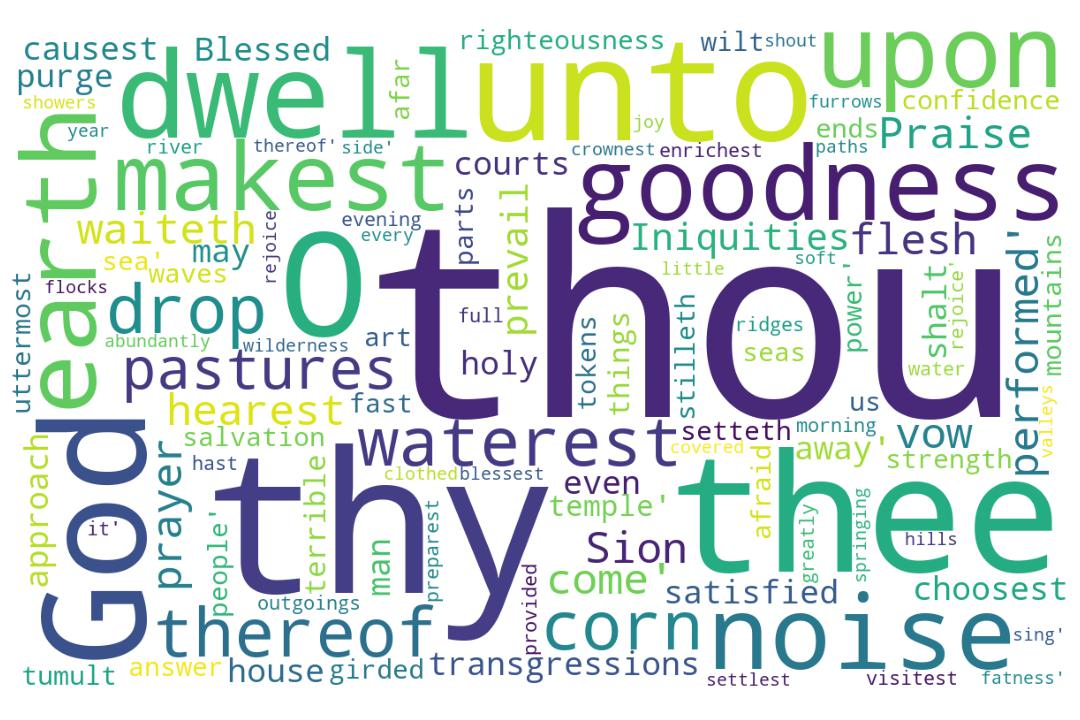
\includegraphics[width=\linewidth]{19OT-Psalms/Psalm65-WordCloud.jpg}
  \caption{Psalm 65 Word Cloud}
  \label{fig:Psalm 65 word Cloud}
\end{figure}


\marginpar{\scriptsize \centering \fcolorbox{bone}{lime}{\textbf{THANKWORTHY}}\\ (Psalm 65:1-13) \begin{compactenum}[I.][8]
    \item \textbf{Grace}  \index[scripture]{Psalms!Psa 065:01--04}(Psa 65:1--4)
    \item \textbf{Goodness}  \index[scripture]{Psalms!Psa 065:04}(Psa 65:4)
    \item \textbf{Greatness}  \index[scripture]{Psalms!Psa 065:05--08}(Psa 65:5--8)
    \item \textbf{Girding}  \index[scripture]{Psalms!Psa 065:06}(Psa 65:6)
    \item \textbf{Grain}  \index[scripture]{Psalms!Psa 065:09--13}(Psa 65:9--13)
    \item \textbf{Gathering}  \index[scripture]{Psalms!Psa 065:09}(Psa 65:9)
    \item \textbf{Gentleness}  \index[scripture]{Psalms!Psa 065:13}(Psa 65:13)
\end{compactenum}}

\footnote{\textcolor[rgb]{0.00,0.25,0.00}{\hyperlink{TOC}{Return to end of Table of Contents.}}}\footnote{\href{https://audiobible.com/bible/psalms_65.html}{\textcolor[cmyk]{0.99998,1,0,0}{Psalm 65 Audio}}}\textcolor[cmyk]{0.99998,1,0,0}{To the chief Musician, A Psalm \emph{and} Song of David.}\\
\\
\textcolor[cmyk]{0.99998,1,0,0}{Praise waiteth for thee, O God, in Sion: and unto thee shall the vow be performed.}\footnote{\textbf{Psalm 22:23-29} - Ye that fear the LORD, praise him; all ye the seed of Jacob, glorify him; and fear him, all ye the seed of Israel. [24] For he hath not despised nor abhorred the affliction of the afflicted; neither hath he hid his face from him; but when he cried unto him, he heard. [25] My praise shall be of thee in the great congregation: I will pay my vows before them that fear him. [26] The meek shall eat and be satisfied: they shall praise the LORD that seek him: your heart shall live for ever. [27] All the ends of the world shall remember and turn unto the LORD: and all the kindreds of the nations shall worship before thee. [28] For the kingdom is the LORD’S: and he is the governor among the nations. [29] All they that be fat upon earth shall eat and worship: all they that go down to the dust shall bow before him: and none can keep alive his own soul.}\footnote{\textbf{Psalm 61:5} -For thou, O God, hast heard my vows: thou hast given me the heritage of those that fear thy name.}
[2] \textcolor[cmyk]{0.99998,1,0,0}{O thou that hearest prayer, unto thee shall all flesh come.}
[3] \textcolor[cmyk]{0.99998,1,0,0}{Iniquities prevail against me: \emph{as} \emph{for} our transgressions, thou shalt purge them away.}
[4] \textcolor[cmyk]{0.99998,1,0,0}{Blessed \emph{is} \emph{the} \emph{man} \emph{whom} \fcolorbox{bone}{lime}{thou choosest}, and causest to approach \emph{unto} \emph{thee,} \emph{that} he may dwell in thy courts: we shall be satisfied with the \fcolorbox{bone}{lime}{goodness} \fcolorbox{bone}{bone}{of} thy house, \emph{even} \fcolorbox{bone}{bone}{of} thy holy temple.}
[5] \textcolor[cmyk]{0.99998,1,0,0}{\emph{By} terrible things in \fcolorbox{bone}{MYGOLD}{righteousness} wilt thou answer us, O God \fcolorbox{bone}{bone}{of} our salvation; \emph{who} \emph{art} the confidence \fcolorbox{bone}{lime}{\fcolorbox{bone}{bone}{of} all the ends \fcolorbox{bone}{bone}{of} the earth}, and \fcolorbox{bone}{bone}{of} them that are afar off \emph{upon} the sea:}
[6] \textcolor[cmyk]{0.99998,1,0,0}{Which by his strength setteth fast the mountains; \emph{being} \fcolorbox{bone}{lime}{girded} with power:}
[7] \textcolor[cmyk]{0.99998,1,0,0}{Which stilleth the noise \fcolorbox{bone}{bone}{of} the seas, the noise \fcolorbox{bone}{bone}{of} their waves, and the tumult \fcolorbox{bone}{bone}{of} the people.}
[8] \textcolor[cmyk]{0.99998,1,0,0}{They also that dwell in the uttermost parts are afraid at thy tokens: thou makest the outgoings \fcolorbox{bone}{bone}{of} the morning and evening to rejoice.}
[9] \textcolor[cmyk]{0.99998,1,0,0}{Thou visitest the earth, and waterest it: thou greatly enrichest it with the river \fcolorbox{bone}{bone}{of} God, \emph{which} is full \fcolorbox{bone}{bone}{of} water: thou preparest them \fcolorbox{bone}{lime}{corn}, when thou hast so provided for it.}
[10] \textcolor[cmyk]{0.99998,1,0,0}{Thou waterest the ridges thereof abundantly: thou settlest the furrows thereof: thou makest it soft with showers: thou blessest the springing thereof.}
[11] \textcolor[cmyk]{0.99998,1,0,0}{Thou crownest the year with thy goodness; and thy paths drop fatness.}
[12] \textcolor[cmyk]{0.99998,1,0,0}{They drop \emph{upon} the pastures \fcolorbox{bone}{bone}{of} the wilderness: and the little hills rejoice on every side.}
[13] \textcolor[cmyk]{0.99998,1,0,0}{The \fcolorbox{bone}{lime}{pastures} are clothed with flocks; the valleys also are covered over with corn; they shout for joy, they also sing.}




\index[NWIV]{16!Psa!Psa 65:1}\index[AWIP]{Praise!Psa!Psa 65:1}\index[AWIP]{waiteth!Psa!Psa 65:1}\index[AWIP]{for!Psa!Psa 65:1}\index[AWIP]{thee!Psa!Psa 65:1}\index[AWIP]{thee!Psa!Psa 65:1 (2)}\index[AWIP]{O!Psa!Psa 65:1}\index[AWIP]{God!Psa!Psa 65:1}\index[AWIP]{in!Psa!Psa 65:1}\index[AWIP]{Sion!Psa!Psa 65:1}\index[AWIP]{and!Psa!Psa 65:1}\index[AWIP]{unto!Psa!Psa 65:1}\index[AWIP]{shall!Psa!Psa 65:1}\index[AWIP]{the!Psa!Psa 65:1}\index[AWIP]{vow!Psa!Psa 65:1}\index[AWIP]{be!Psa!Psa 65:1}\index[AWIP]{performed!Psa!Psa 65:1}

\index[NWIV]{11!Psa!Psa 65:2}\index[AWIP]{O!Psa!Psa 65:2}\index[AWIP]{thou!Psa!Psa 65:2}\index[AWIP]{that!Psa!Psa 65:2}\index[AWIP]{hearest!Psa!Psa 65:2}\index[AWIP]{prayer!Psa!Psa 65:2}\index[AWIP]{unto!Psa!Psa 65:2}\index[AWIP]{thee!Psa!Psa 65:2}\index[AWIP]{shall!Psa!Psa 65:2}\index[AWIP]{all!Psa!Psa 65:2}\index[AWIP]{flesh!Psa!Psa 65:2}\index[AWIP]{come!Psa!Psa 65:2}

\index[NWIV]{13!Psa!Psa 65:3}\index[AWIP]{Iniquities!Psa!Psa 65:3}\index[AWIP]{prevail!Psa!Psa 65:3}\index[AWIP]{against!Psa!Psa 65:3}\index[AWIP]{me!Psa!Psa 65:3}\index[AWIP]{\emph{as}!Psa!Psa 65:3}\index[AWIP]{\emph{for}!Psa!Psa 65:3}\index[AWIP]{our!Psa!Psa 65:3}\index[AWIP]{transgressions!Psa!Psa 65:3}\index[AWIP]{thou!Psa!Psa 65:3}\index[AWIP]{shalt!Psa!Psa 65:3}\index[AWIP]{purge!Psa!Psa 65:3}\index[AWIP]{them!Psa!Psa 65:3}\index[AWIP]{away!Psa!Psa 65:3}\index[AWIP]{\emph{as}!Psa!Psa 65:3}\index[AWIP]{\emph{for}!Psa!Psa 65:3}

\index[NWIV]{35!Psa!Psa 65:4}\index[AWIP]{Blessed!Psa!Psa 65:4}\index[AWIP]{\emph{is}!Psa!Psa 65:4}\index[AWIP]{\emph{the}!Psa!Psa 65:4}\index[AWIP]{\emph{man}!Psa!Psa 65:4}\index[AWIP]{\emph{whom}!Psa!Psa 65:4}\index[AWIP]{thou!Psa!Psa 65:4}\index[AWIP]{choosest!Psa!Psa 65:4}\index[AWIP]{and!Psa!Psa 65:4}\index[AWIP]{causest!Psa!Psa 65:4}\index[AWIP]{to!Psa!Psa 65:4}\index[AWIP]{approach!Psa!Psa 65:4}\index[AWIP]{\emph{unto}!Psa!Psa 65:4}\index[AWIP]{\emph{thee}!Psa!Psa 65:4}\index[AWIP]{\emph{that}!Psa!Psa 65:4}\index[AWIP]{he!Psa!Psa 65:4}\index[AWIP]{may!Psa!Psa 65:4}\index[AWIP]{dwell!Psa!Psa 65:4}\index[AWIP]{in!Psa!Psa 65:4}\index[AWIP]{thy!Psa!Psa 65:4}\index[AWIP]{thy!Psa!Psa 65:4 (2)}\index[AWIP]{thy!Psa!Psa 65:4 (3)}\index[AWIP]{courts!Psa!Psa 65:4}\index[AWIP]{we!Psa!Psa 65:4}\index[AWIP]{shall!Psa!Psa 65:4}\index[AWIP]{be!Psa!Psa 65:4}\index[AWIP]{satisfied!Psa!Psa 65:4}\index[AWIP]{with!Psa!Psa 65:4}\index[AWIP]{the!Psa!Psa 65:4}\index[AWIP]{goodness!Psa!Psa 65:4}\index[AWIP]{of!Psa!Psa 65:4}\index[AWIP]{of!Psa!Psa 65:4 (2)}\index[AWIP]{house!Psa!Psa 65:4}\index[AWIP]{\emph{even}!Psa!Psa 65:4}\index[AWIP]{holy!Psa!Psa 65:4}\index[AWIP]{temple!Psa!Psa 65:4}\index[AWIP]{\emph{is}!Psa!Psa 65:4}\index[AWIP]{\emph{the}!Psa!Psa 65:4}\index[AWIP]{\emph{man}!Psa!Psa 65:4}\index[AWIP]{\emph{whom}!Psa!Psa 65:4}\index[AWIP]{\emph{unto}!Psa!Psa 65:4}\index[AWIP]{\emph{thee}!Psa!Psa 65:4}\index[AWIP]{\emph{that}!Psa!Psa 65:4}\index[AWIP]{\emph{even}!Psa!Psa 65:4}

\index[NWIV]{35!Psa!Psa 65:5}\index[AWIP]{\emph{By}!Psa!Psa 65:5}\index[AWIP]{terrible!Psa!Psa 65:5}\index[AWIP]{things!Psa!Psa 65:5}\index[AWIP]{in!Psa!Psa 65:5}\index[AWIP]{righteousness!Psa!Psa 65:5}\index[AWIP]{wilt!Psa!Psa 65:5}\index[AWIP]{thou!Psa!Psa 65:5}\index[AWIP]{answer!Psa!Psa 65:5}\index[AWIP]{us!Psa!Psa 65:5}\index[AWIP]{O!Psa!Psa 65:5}\index[AWIP]{God!Psa!Psa 65:5}\index[AWIP]{of!Psa!Psa 65:5}\index[AWIP]{of!Psa!Psa 65:5 (2)}\index[AWIP]{of!Psa!Psa 65:5 (3)}\index[AWIP]{of!Psa!Psa 65:5 (4)}\index[AWIP]{our!Psa!Psa 65:5}\index[AWIP]{salvation!Psa!Psa 65:5}\index[AWIP]{\emph{who}!Psa!Psa 65:5}\index[AWIP]{\emph{art}!Psa!Psa 65:5}\index[AWIP]{the!Psa!Psa 65:5}\index[AWIP]{the!Psa!Psa 65:5 (2)}\index[AWIP]{the!Psa!Psa 65:5 (3)}\index[AWIP]{the!Psa!Psa 65:5 (4)}\index[AWIP]{confidence!Psa!Psa 65:5}\index[AWIP]{all!Psa!Psa 65:5}\index[AWIP]{ends!Psa!Psa 65:5}\index[AWIP]{earth!Psa!Psa 65:5}\index[AWIP]{and!Psa!Psa 65:5}\index[AWIP]{them!Psa!Psa 65:5}\index[AWIP]{that!Psa!Psa 65:5}\index[AWIP]{are!Psa!Psa 65:5}\index[AWIP]{afar!Psa!Psa 65:5}\index[AWIP]{off!Psa!Psa 65:5}\index[AWIP]{\emph{upon}!Psa!Psa 65:5}\index[AWIP]{sea!Psa!Psa 65:5}\index[AWIP]{\emph{By}!Psa!Psa 65:5}\index[AWIP]{\emph{who}!Psa!Psa 65:5}\index[AWIP]{\emph{art}!Psa!Psa 65:5}\index[AWIP]{\emph{upon}!Psa!Psa 65:5}

\index[NWIV]{12!Psa!Psa 65:6}\index[AWIP]{Which!Psa!Psa 65:6}\index[AWIP]{by!Psa!Psa 65:6}\index[AWIP]{his!Psa!Psa 65:6}\index[AWIP]{strength!Psa!Psa 65:6}\index[AWIP]{setteth!Psa!Psa 65:6}\index[AWIP]{fast!Psa!Psa 65:6}\index[AWIP]{the!Psa!Psa 65:6}\index[AWIP]{mountains!Psa!Psa 65:6}\index[AWIP]{\emph{being}!Psa!Psa 65:6}\index[AWIP]{girded!Psa!Psa 65:6}\index[AWIP]{with!Psa!Psa 65:6}\index[AWIP]{power!Psa!Psa 65:6}\index[AWIP]{\emph{being}!Psa!Psa 65:6}

\index[NWIV]{18!Psa!Psa 65:7}\index[AWIP]{Which!Psa!Psa 65:7}\index[AWIP]{stilleth!Psa!Psa 65:7}\index[AWIP]{the!Psa!Psa 65:7}\index[AWIP]{the!Psa!Psa 65:7 (2)}\index[AWIP]{the!Psa!Psa 65:7 (3)}\index[AWIP]{the!Psa!Psa 65:7 (4)}\index[AWIP]{the!Psa!Psa 65:7 (5)}\index[AWIP]{noise!Psa!Psa 65:7}\index[AWIP]{noise!Psa!Psa 65:7 (2)}\index[AWIP]{of!Psa!Psa 65:7}\index[AWIP]{of!Psa!Psa 65:7 (2)}\index[AWIP]{of!Psa!Psa 65:7 (3)}\index[AWIP]{seas!Psa!Psa 65:7}\index[AWIP]{their!Psa!Psa 65:7}\index[AWIP]{waves!Psa!Psa 65:7}\index[AWIP]{and!Psa!Psa 65:7}\index[AWIP]{tumult!Psa!Psa 65:7}\index[AWIP]{people!Psa!Psa 65:7}

\index[NWIV]{24!Psa!Psa 65:8}\index[AWIP]{They!Psa!Psa 65:8}\index[AWIP]{also!Psa!Psa 65:8}\index[AWIP]{that!Psa!Psa 65:8}\index[AWIP]{dwell!Psa!Psa 65:8}\index[AWIP]{in!Psa!Psa 65:8}\index[AWIP]{the!Psa!Psa 65:8}\index[AWIP]{the!Psa!Psa 65:8 (2)}\index[AWIP]{the!Psa!Psa 65:8 (3)}\index[AWIP]{uttermost!Psa!Psa 65:8}\index[AWIP]{parts!Psa!Psa 65:8}\index[AWIP]{are!Psa!Psa 65:8}\index[AWIP]{afraid!Psa!Psa 65:8}\index[AWIP]{at!Psa!Psa 65:8}\index[AWIP]{thy!Psa!Psa 65:8}\index[AWIP]{tokens!Psa!Psa 65:8}\index[AWIP]{thou!Psa!Psa 65:8}\index[AWIP]{makest!Psa!Psa 65:8}\index[AWIP]{outgoings!Psa!Psa 65:8}\index[AWIP]{of!Psa!Psa 65:8}\index[AWIP]{morning!Psa!Psa 65:8}\index[AWIP]{and!Psa!Psa 65:8}\index[AWIP]{evening!Psa!Psa 65:8}\index[AWIP]{to!Psa!Psa 65:8}\index[AWIP]{rejoice!Psa!Psa 65:8}

\index[NWIV]{32!Psa!Psa 65:9}\index[AWIP]{Thou!Psa!Psa 65:9}\index[AWIP]{visitest!Psa!Psa 65:9}\index[AWIP]{the!Psa!Psa 65:9}\index[AWIP]{the!Psa!Psa 65:9 (2)}\index[AWIP]{earth!Psa!Psa 65:9}\index[AWIP]{and!Psa!Psa 65:9}\index[AWIP]{waterest!Psa!Psa 65:9}\index[AWIP]{it!Psa!Psa 65:9}\index[AWIP]{it!Psa!Psa 65:9 (2)}\index[AWIP]{it!Psa!Psa 65:9 (3)}\index[AWIP]{thou!Psa!Psa 65:9}\index[AWIP]{thou!Psa!Psa 65:9 (2)}\index[AWIP]{thou!Psa!Psa 65:9 (3)}\index[AWIP]{greatly!Psa!Psa 65:9}\index[AWIP]{enrichest!Psa!Psa 65:9}\index[AWIP]{with!Psa!Psa 65:9}\index[AWIP]{river!Psa!Psa 65:9}\index[AWIP]{of!Psa!Psa 65:9}\index[AWIP]{of!Psa!Psa 65:9 (2)}\index[AWIP]{God!Psa!Psa 65:9}\index[AWIP]{\emph{which}!Psa!Psa 65:9}\index[AWIP]{is!Psa!Psa 65:9}\index[AWIP]{full!Psa!Psa 65:9}\index[AWIP]{water!Psa!Psa 65:9}\index[AWIP]{preparest!Psa!Psa 65:9}\index[AWIP]{them!Psa!Psa 65:9}\index[AWIP]{corn!Psa!Psa 65:9}\index[AWIP]{when!Psa!Psa 65:9}\index[AWIP]{hast!Psa!Psa 65:9}\index[AWIP]{so!Psa!Psa 65:9}\index[AWIP]{provided!Psa!Psa 65:9}\index[AWIP]{for!Psa!Psa 65:9}\index[AWIP]{\emph{which}!Psa!Psa 65:9}

\index[NWIV]{22!Psa!Psa 65:10}\index[AWIP]{Thou!Psa!Psa 65:10}\index[AWIP]{waterest!Psa!Psa 65:10}\index[AWIP]{the!Psa!Psa 65:10}\index[AWIP]{the!Psa!Psa 65:10 (2)}\index[AWIP]{the!Psa!Psa 65:10 (3)}\index[AWIP]{ridges!Psa!Psa 65:10}\index[AWIP]{thereof!Psa!Psa 65:10}\index[AWIP]{thereof!Psa!Psa 65:10 (2)}\index[AWIP]{thereof!Psa!Psa 65:10 (3)}\index[AWIP]{abundantly!Psa!Psa 65:10}\index[AWIP]{thou!Psa!Psa 65:10}\index[AWIP]{thou!Psa!Psa 65:10 (2)}\index[AWIP]{thou!Psa!Psa 65:10 (3)}\index[AWIP]{settlest!Psa!Psa 65:10}\index[AWIP]{furrows!Psa!Psa 65:10}\index[AWIP]{makest!Psa!Psa 65:10}\index[AWIP]{it!Psa!Psa 65:10}\index[AWIP]{soft!Psa!Psa 65:10}\index[AWIP]{with!Psa!Psa 65:10}\index[AWIP]{showers!Psa!Psa 65:10}\index[AWIP]{blessest!Psa!Psa 65:10}\index[AWIP]{springing!Psa!Psa 65:10}

\index[NWIV]{12!Psa!Psa 65:11}\index[AWIP]{Thou!Psa!Psa 65:11}\index[AWIP]{crownest!Psa!Psa 65:11}\index[AWIP]{the!Psa!Psa 65:11}\index[AWIP]{year!Psa!Psa 65:11}\index[AWIP]{with!Psa!Psa 65:11}\index[AWIP]{thy!Psa!Psa 65:11}\index[AWIP]{thy!Psa!Psa 65:11 (2)}\index[AWIP]{goodness!Psa!Psa 65:11}\index[AWIP]{and!Psa!Psa 65:11}\index[AWIP]{paths!Psa!Psa 65:11}\index[AWIP]{drop!Psa!Psa 65:11}\index[AWIP]{fatness!Psa!Psa 65:11}

\index[NWIV]{16!Psa!Psa 65:12}\index[AWIP]{They!Psa!Psa 65:12}\index[AWIP]{drop!Psa!Psa 65:12}\index[AWIP]{\emph{upon}!Psa!Psa 65:12}\index[AWIP]{the!Psa!Psa 65:12}\index[AWIP]{the!Psa!Psa 65:12 (2)}\index[AWIP]{the!Psa!Psa 65:12 (3)}\index[AWIP]{pastures!Psa!Psa 65:12}\index[AWIP]{of!Psa!Psa 65:12}\index[AWIP]{wilderness!Psa!Psa 65:12}\index[AWIP]{and!Psa!Psa 65:12}\index[AWIP]{little!Psa!Psa 65:12}\index[AWIP]{hills!Psa!Psa 65:12}\index[AWIP]{rejoice!Psa!Psa 65:12}\index[AWIP]{on!Psa!Psa 65:12}\index[AWIP]{every!Psa!Psa 65:12}\index[AWIP]{side!Psa!Psa 65:12}\index[AWIP]{\emph{upon}!Psa!Psa 65:12}

\index[NWIV]{21!Psa!Psa 65:13}\index[AWIP]{The!Psa!Psa 65:13}\index[AWIP]{pastures!Psa!Psa 65:13}\index[AWIP]{are!Psa!Psa 65:13}\index[AWIP]{are!Psa!Psa 65:13 (2)}\index[AWIP]{clothed!Psa!Psa 65:13}\index[AWIP]{with!Psa!Psa 65:13}\index[AWIP]{with!Psa!Psa 65:13 (2)}\index[AWIP]{flocks!Psa!Psa 65:13}\index[AWIP]{the!Psa!Psa 65:13}\index[AWIP]{valleys!Psa!Psa 65:13}\index[AWIP]{also!Psa!Psa 65:13}\index[AWIP]{also!Psa!Psa 65:13 (2)}\index[AWIP]{covered!Psa!Psa 65:13}\index[AWIP]{over!Psa!Psa 65:13}\index[AWIP]{corn!Psa!Psa 65:13}\index[AWIP]{they!Psa!Psa 65:13}\index[AWIP]{they!Psa!Psa 65:13 (2)}\index[AWIP]{shout!Psa!Psa 65:13}\index[AWIP]{for!Psa!Psa 65:13}\index[AWIP]{joy!Psa!Psa 65:13}\index[AWIP]{sing!Psa!Psa 65:13}


\section{Psalm 65 Outlines}

\subsection{My Outlines}

\subsubsection{Thankworthy}

\index[speaker]{Keith Anthony!Psalm 065 (Thankworthy)}
\index[series]{Psalms (Keith Anthony)!Psalm 065 (Thankworthy)}
\index[date]{2017/08/08!Psalm 065 (Thankworthy) (Keith Anthony)}

\begin{compactenum}[I.][7]
    \item \textbf{Grace}  \index[scripture]{Psalms!Psa 065:01--04}(Psa 65:1--4)
    \item \textbf{Goodness}  \index[scripture]{Psalms!Psa 065:04}(Psa 65:4)
    \item \textbf{Greatness}  \index[scripture]{Psalms!Psa 065:05--08}(Psa 65:5--8)
    \item \textbf{Girding}  \index[scripture]{Psalms!Psa 065:06}(Psa 65:6)
    \item \textbf{Grain}  \index[scripture]{Psalms!Psa 065:09--13}(Psa 65:9--13)
    \item \textbf{Gathering}  \index[scripture]{Psalms!Psa 065:09}(Psa 65:9)
    \item \textbf{Gentleness}  \index[scripture]{Psalms!Psa 065:13}(Psa 65:13)
\end{compactenum}


\subsection{Outlines from Others}


\section{Psalm 65 Comments}

\subsection{Numeric Nuggets}
Verse 3 has 13 words and 13 unique words. The word ``of'' is used 13 times in Psalm 65. The 13-letter word ``righteousness'' is used in the psalm.

\chapter{Proverb 6}

\begin{figure}
  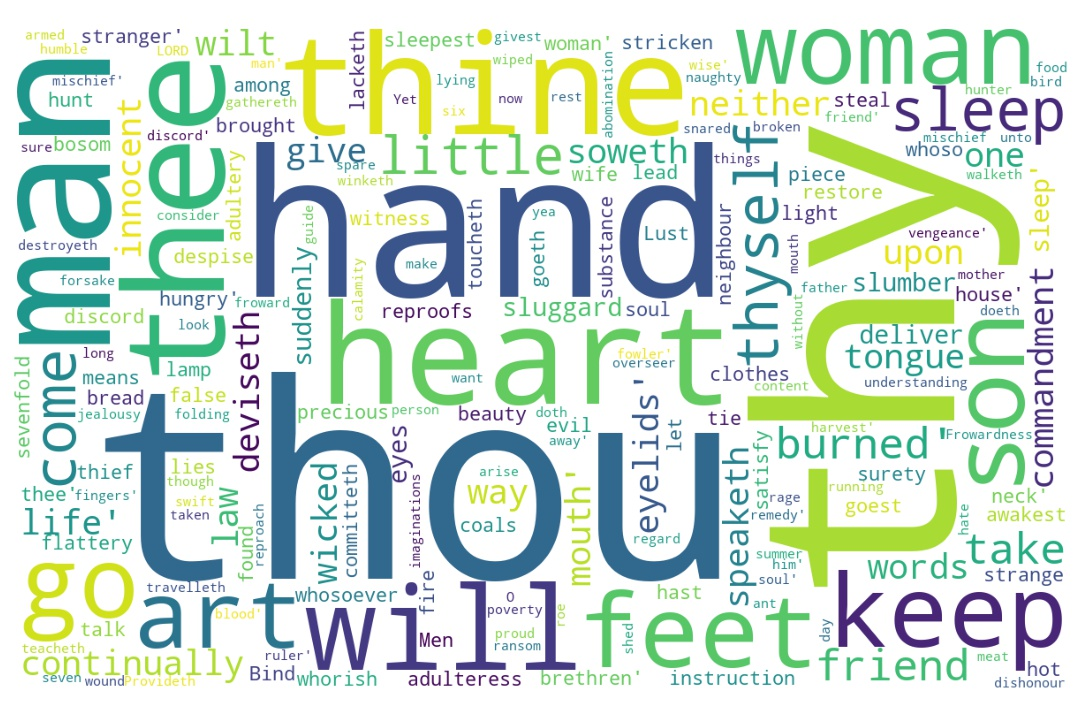
\includegraphics[width=\linewidth]{20OT-Proverbs/Proverb6-WordCloud.jpg}
  \caption{Proverb 6 Word Cloud}
  \label{fig:Proverb 6 Word Cloud}
\end{figure}

\marginpar{\scriptsize \centering \fcolorbox{bone}{lime}{\textbf{THINGS NOT TO DO}}\\ (Proverb 6:1-5) \begin{compactenum}[I.][8]
    \item \textbf{Don't Become Liable} \index[scripture]{Proverbs!Pro 06:01-03}(Proverbs 6:1-3) - and when you do, get out of that liability
    \item \textbf{Don't Became Lazy} \index[scripture]{Proverbs!Pro 06:04}(Pro 6:4) 
    \item \textbf{Don't Lie} \index[scripture]{Proverbs!Pro 06:12, 19} (Pro 6:12, 19) 
    \item \textbf{Don't get an Evil Longing}  \index[scripture]{Proverbs!Pro 06:14}(Pro 6:14) 
    \item \textbf{Don't Get a Proud Look} \index[scripture]{Proverbs!Pro 06:17}(Pro 6:17)
    \item \textbf{Don't Yield to Lust} \index[scripture]{Proverbs!Pro 06:25}(Pro 6:25)
    \item \textbf{Don't Lack Understanding} \index[scripture]{Proverbs!Pro 06:32}(Pro 6:32)
\end{compactenum}}

\footnote{\textcolor[cmyk]{0.99998,1,0,0}{\hyperlink{TOC}{Return to end of Table of Contents.}}}\footnote{\href{https://audiobible.com/bible/proverbs_6.html}{\textcolor[cmyk]{0.99998,1,0,0}{Proverbs Audio}}}\textcolor[cmyk]{0.99998,1,0,0}{My son, if thou be \fcolorbox{bone}{lime}{surety} for thy friend, \emph{if} thou hast stricken thy hand with a stranger,}\
[2] \textcolor[cmyk]{0.99998,1,0,0}{Thou art snared with the words of thy mouth, thou art taken with the words of thy mouth.}\
[3] \textcolor[cmyk]{0.99998,1,0,0}{Do this now, my son, and deliver thyself, when thou art come into the hand of thy friend; go, humble thyself, and make sure thy friend.}
[4] \textcolor[cmyk]{0.99998,1,0,0}{Give not sleep to thine eyes, nor \fcolorbox{bone}{lime}{slumber} to thine eyelids.}
[5] \textcolor[cmyk]{0.99998,1,0,0}{Deliver thyself as a roe from the hand \emph{of} \emph{the} \emph{hunter}, and as a bird from the hand of the fowler.}
[6] \textcolor[cmyk]{0.99998,1,0,0}{Go to the ant, thou sluggard; consider her ways, and be wise:}
[7] \textcolor[cmyk]{0.99998,1,0,0}{Which having no guide, overseer, or ruler,}
[8] \textcolor[cmyk]{0.99998,1,0,0}{Provideth her meat in the summer, \emph{and} gathereth her food in the harvest.}
[9] \textcolor[cmyk]{0.99998,1,0,0}{How long wilt thou sleep, O sluggard? when wilt thou arise out of thy sleep?}
[10] \textcolor[cmyk]{0.99998,1,0,0}{\emph{Yet} a little sleep, a little slumber, a little folding of the hands to sleep:}
[11] \textcolor[cmyk]{0.99998,1,0,0}{So shall thy poverty come as one that travelleth, and thy want as an armed man.}
[12] \textcolor[cmyk]{0.99998,1,0,0}{A naughty person, a wicked man, walketh with a \fcolorbox{bone}{lime}{froward} mouth.}
[13] \textcolor[cmyk]{0.99998,1,0,0}{He winketh with \fcolorbox{bone}{bone}{his} eyes, he speaketh with \fcolorbox{bone}{bone}{his} feet, he teacheth with \fcolorbox{bone}{bone}{his} fingers;}
[14] \textcolor[cmyk]{0.99998,1,0,0}{Frowardness \emph{is} \fcolorbox{bone}{lime}{in \fcolorbox{bone}{bone}{his} heart}, he deviseth mischief continually; he soweth discord.}
[15] \textcolor[cmyk]{0.99998,1,0,0}{Therefore shall \fcolorbox{bone}{bone}{his} calamity come suddenly; suddenly shall he be broken without remedy.}
[16] \textcolor[cmyk]{0.99998,1,0,0}{These six \emph{things} doth the LORD hate: yea, seven \emph{are} an abomination unto him:} %\marginpar{\scriptsize %\textcolor[rgb]{0.00,0.545,0.269}{$\rightarrow$7 Abominations: 
%\begin{compactenum}
%	\item A proud look,
%	\item a lying tongue,
%	\item hands that shed innocent blood,
%	\item An heart that deviseth wicked imaginations,
%	\item feet that be swift in running to mischief,
%	\item A false witness that speaketh lies, and
%	\item he that soweth discord among brethren.
%\end{compactenum}}}
[17] \textcolor[cmyk]{0.99998,1,0,0}{A \fcolorbox{bone}{lime}{proud look}, a lying tongue, and hands that shed innocent blood,}
[18] \textcolor[cmyk]{0.99998,1,0,0}{An heart that deviseth wicked imaginations, feet that be swift in running to mischief,}
[19] \textcolor[cmyk]{0.99998,1,0,0}{A false witness \emph{that} speaketh lies, and he that soweth discord among brethren.}
[20] \textcolor[cmyk]{0.99998,1,0,0}{My son, keep thy father's commandment, and forsake not the law of thy mother:}
[21] \textcolor[cmyk]{0.99998,1,0,0}{Bind them continually upon thine heart, \emph{and} tie them about thy neck.}
[22] \textcolor[cmyk]{0.99998,1,0,0}{When thou goest, it shall lead thee; when thou sleepest, it shall keep thee; and \emph{when} thou awakest, it shall talk with thee.}
[23] \textcolor[cmyk]{0.99998,1,0,0}{For the commandment \emph{is} a lamp; and the law \emph{is} light; and reproofs of instruction \emph{are} the way of life:}\footnote{\textbf{Psalm 119:105} - Thy word is a lamp unto my feet, and a light unto my path.}
[24] \textcolor[cmyk]{0.99998,1,0,0}{To keep thee from the evil woman, from the flattery of the tongue of a strange woman.}
[25] \textcolor[cmyk]{0.99998,1,0,0}{\fcolorbox{bone}{lime}{Lust not} after her beauty in thine heart; neither let her take thee with her eyelids.}
[26] \textcolor[cmyk]{0.99998,1,0,0}{For by means of a whorish woman \emph{a} \emph{man} \emph{is} \emph{brought} to a piece of bread: and the adulteress will hunt for the precious life.}
[27] \textcolor[cmyk]{0.99998,1,0,0}{Can a man take fire in \fcolorbox{bone}{bone}{his} bosom, and \fcolorbox{bone}{bone}{his} clothes not be burned?}
[28] \textcolor[cmyk]{0.99998,1,0,0}{Can one go upon hot coals, and \fcolorbox{bone}{bone}{his} feet not be burned?}
[29] \textcolor[cmyk]{0.99998,1,0,0}{So he that goeth in to \fcolorbox{bone}{bone}{his} neighbour's wife; whosoever toucheth her shall not be innocent.}\footnote{\textbf{1 Corinthians 7:1} - Now concerning the things whereof ye wrote unto me: It is good for a man not to touch a woman.}
[30] \textcolor[cmyk]{0.99998,1,0,0}{\emph{Men} do not despise a thief, if he steal to satisfy \fcolorbox{bone}{bone}{his} soul when he is hungry;}
[31] \textcolor[cmyk]{0.99998,1,0,0}{But \emph{if} he be found, he shall restore sevenfold; he shall give all the substance of \fcolorbox{bone}{bone}{his} house.}
[32] \textcolor[cmyk]{0.99998,1,0,0}{\emph{But} whoso committeth adultery with a woman \fcolorbox{bone}{lime}{lacketh \fcolorbox{bone}{MYGOLD}{understanding}}: he \emph{that} doeth it destroyeth \fcolorbox{bone}{bone}{his} own soul.}
[33] \textcolor[cmyk]{0.99998,1,0,0}{A wound and dishonour shall he get; and \fcolorbox{bone}{bone}{his} reproach shall not be wiped away.}
[34] \textcolor[cmyk]{0.99998,1,0,0}{For jealousy \emph{is} the rage of a man: therefore he will not spare in the day of vengeance.}
[35] \textcolor[cmyk]{0.99998,1,0,0}{He will not regard any ransom; neither will he rest content, though thou givest many gifts.}






\index[NWIV]{18!Proverbs!Pro 6:1}\index[AWIP]{My!Proverbs!Pro 6:1}\index[AWIP]{son!Proverbs!Pro 6:1}\index[AWIP]{if!Proverbs!Pro 6:1}\index[AWIP]{thou!Proverbs!Pro 6:1}\index[AWIP]{thou!Proverbs!Pro 6:1 (2)}\index[AWIP]{be!Proverbs!Pro 6:1}\index[AWIP]{surety!Proverbs!Pro 6:1}\index[AWIP]{for!Proverbs!Pro 6:1}\index[AWIP]{thy!Proverbs!Pro 6:1}\index[AWIP]{thy!Proverbs!Pro 6:1 (2)}\index[AWIP]{friend!Proverbs!Pro 6:1}\index[AWIP]{\emph{if}!Proverbs!Pro 6:1}\index[AWIP]{hast!Proverbs!Pro 6:1}\index[AWIP]{stricken!Proverbs!Pro 6:1}\index[AWIP]{hand!Proverbs!Pro 6:1}\index[AWIP]{with!Proverbs!Pro 6:1}\index[AWIP]{a!Proverbs!Pro 6:1}\index[AWIP]{stranger!Proverbs!Pro 6:1}\index[AWIP]{\emph{if}!Proverbs!Pro 6:1}

\index[NWIV]{18!Proverbs!Pro 6:2}\index[AWIP]{Thou!Proverbs!Pro 6:2}\index[AWIP]{art!Proverbs!Pro 6:2}\index[AWIP]{art!Proverbs!Pro 6:2 (2)}\index[AWIP]{snared!Proverbs!Pro 6:2}\index[AWIP]{with!Proverbs!Pro 6:2}\index[AWIP]{with!Proverbs!Pro 6:2 (2)}\index[AWIP]{the!Proverbs!Pro 6:2}\index[AWIP]{the!Proverbs!Pro 6:2 (2)}\index[AWIP]{words!Proverbs!Pro 6:2}\index[AWIP]{words!Proverbs!Pro 6:2 (2)}\index[AWIP]{of!Proverbs!Pro 6:2}\index[AWIP]{of!Proverbs!Pro 6:2 (2)}\index[AWIP]{thy!Proverbs!Pro 6:2}\index[AWIP]{thy!Proverbs!Pro 6:2 (2)}\index[AWIP]{mouth!Proverbs!Pro 6:2}\index[AWIP]{mouth!Proverbs!Pro 6:2 (2)}\index[AWIP]{thou!Proverbs!Pro 6:2}\index[AWIP]{taken!Proverbs!Pro 6:2}

\index[NWIV]{26!Proverbs!Pro 6:3}\index[AWIP]{Do!Proverbs!Pro 6:3}\index[AWIP]{this!Proverbs!Pro 6:3}\index[AWIP]{now!Proverbs!Pro 6:3}\index[AWIP]{my!Proverbs!Pro 6:3}\index[AWIP]{son!Proverbs!Pro 6:3}\index[AWIP]{and!Proverbs!Pro 6:3}\index[AWIP]{and!Proverbs!Pro 6:3 (2)}\index[AWIP]{deliver!Proverbs!Pro 6:3}\index[AWIP]{thyself!Proverbs!Pro 6:3}\index[AWIP]{thyself!Proverbs!Pro 6:3 (2)}\index[AWIP]{when!Proverbs!Pro 6:3}\index[AWIP]{thou!Proverbs!Pro 6:3}\index[AWIP]{art!Proverbs!Pro 6:3}\index[AWIP]{come!Proverbs!Pro 6:3}\index[AWIP]{into!Proverbs!Pro 6:3}\index[AWIP]{the!Proverbs!Pro 6:3}\index[AWIP]{hand!Proverbs!Pro 6:3}\index[AWIP]{of!Proverbs!Pro 6:3}\index[AWIP]{thy!Proverbs!Pro 6:3}\index[AWIP]{thy!Proverbs!Pro 6:3 (2)}\index[AWIP]{friend!Proverbs!Pro 6:3}\index[AWIP]{friend!Proverbs!Pro 6:3 (2)}\index[AWIP]{go!Proverbs!Pro 6:3}\index[AWIP]{humble!Proverbs!Pro 6:3}\index[AWIP]{make!Proverbs!Pro 6:3}\index[AWIP]{sure!Proverbs!Pro 6:3}

\index[NWIV]{11!Proverbs!Pro 6:4}\index[AWIP]{Give!Proverbs!Pro 6:4}\index[AWIP]{not!Proverbs!Pro 6:4}\index[AWIP]{sleep!Proverbs!Pro 6:4}\index[AWIP]{to!Proverbs!Pro 6:4}\index[AWIP]{to!Proverbs!Pro 6:4 (2)}\index[AWIP]{thine!Proverbs!Pro 6:4}\index[AWIP]{thine!Proverbs!Pro 6:4 (2)}\index[AWIP]{eyes!Proverbs!Pro 6:4}\index[AWIP]{nor!Proverbs!Pro 6:4}\index[AWIP]{slumber!Proverbs!Pro 6:4}\index[AWIP]{eyelids!Proverbs!Pro 6:4}

\index[NWIV]{21!Proverbs!Pro 6:5}\index[AWIP]{Deliver!Proverbs!Pro 6:5}\index[AWIP]{thyself!Proverbs!Pro 6:5}\index[AWIP]{as!Proverbs!Pro 6:5}\index[AWIP]{as!Proverbs!Pro 6:5 (2)}\index[AWIP]{a!Proverbs!Pro 6:5}\index[AWIP]{a!Proverbs!Pro 6:5 (2)}\index[AWIP]{roe!Proverbs!Pro 6:5}\index[AWIP]{from!Proverbs!Pro 6:5}\index[AWIP]{from!Proverbs!Pro 6:5 (2)}\index[AWIP]{the!Proverbs!Pro 6:5}\index[AWIP]{the!Proverbs!Pro 6:5 (2)}\index[AWIP]{the!Proverbs!Pro 6:5 (3)}\index[AWIP]{hand!Proverbs!Pro 6:5}\index[AWIP]{hand!Proverbs!Pro 6:5 (2)}\index[AWIP]{\emph{of}!Proverbs!Pro 6:5}\index[AWIP]{\emph{the}!Proverbs!Pro 6:5}\index[AWIP]{\emph{hunter}!Proverbs!Pro 6:5}\index[AWIP]{and!Proverbs!Pro 6:5}\index[AWIP]{bird!Proverbs!Pro 6:5}\index[AWIP]{of!Proverbs!Pro 6:5}\index[AWIP]{fowler!Proverbs!Pro 6:5}\index[AWIP]{\emph{of}!Proverbs!Pro 6:5}\index[AWIP]{\emph{the}!Proverbs!Pro 6:5}\index[AWIP]{\emph{hunter}!Proverbs!Pro 6:5}

\index[NWIV]{12!Proverbs!Pro 6:6}\index[AWIP]{Go!Proverbs!Pro 6:6}\index[AWIP]{to!Proverbs!Pro 6:6}\index[AWIP]{the!Proverbs!Pro 6:6}\index[AWIP]{ant!Proverbs!Pro 6:6}\index[AWIP]{thou!Proverbs!Pro 6:6}\index[AWIP]{sluggard!Proverbs!Pro 6:6}\index[AWIP]{consider!Proverbs!Pro 6:6}\index[AWIP]{her!Proverbs!Pro 6:6}\index[AWIP]{ways!Proverbs!Pro 6:6}\index[AWIP]{and!Proverbs!Pro 6:6}\index[AWIP]{be!Proverbs!Pro 6:6}\index[AWIP]{wise!Proverbs!Pro 6:6}

\index[NWIV]{7!Proverbs!Pro 6:7}\index[AWIP]{Which!Proverbs!Pro 6:7}\index[AWIP]{having!Proverbs!Pro 6:7}\index[AWIP]{no!Proverbs!Pro 6:7}\index[AWIP]{guide!Proverbs!Pro 6:7}\index[AWIP]{overseer!Proverbs!Pro 6:7}\index[AWIP]{or!Proverbs!Pro 6:7}\index[AWIP]{ruler!Proverbs!Pro 6:7}

\index[NWIV]{13!Proverbs!Pro 6:8}\index[AWIP]{Provideth!Proverbs!Pro 6:8}\index[AWIP]{her!Proverbs!Pro 6:8}\index[AWIP]{her!Proverbs!Pro 6:8 (2)}\index[AWIP]{meat!Proverbs!Pro 6:8}\index[AWIP]{in!Proverbs!Pro 6:8}\index[AWIP]{in!Proverbs!Pro 6:8 (2)}\index[AWIP]{the!Proverbs!Pro 6:8}\index[AWIP]{the!Proverbs!Pro 6:8 (2)}\index[AWIP]{summer!Proverbs!Pro 6:8}\index[AWIP]{\emph{and}!Proverbs!Pro 6:8}\index[AWIP]{gathereth!Proverbs!Pro 6:8}\index[AWIP]{food!Proverbs!Pro 6:8}\index[AWIP]{harvest!Proverbs!Pro 6:8}\index[AWIP]{\emph{and}!Proverbs!Pro 6:8}

\index[NWIV]{15!Proverbs!Pro 6:9}\index[AWIP]{How!Proverbs!Pro 6:9}\index[AWIP]{long!Proverbs!Pro 6:9}\index[AWIP]{wilt!Proverbs!Pro 6:9}\index[AWIP]{wilt!Proverbs!Pro 6:9 (2)}\index[AWIP]{thou!Proverbs!Pro 6:9}\index[AWIP]{thou!Proverbs!Pro 6:9 (2)}\index[AWIP]{sleep!Proverbs!Pro 6:9}\index[AWIP]{O!Proverbs!Pro 6:9}\index[AWIP]{sluggard?!Proverbs!Pro 6:9}\index[AWIP]{when!Proverbs!Pro 6:9}\index[AWIP]{arise!Proverbs!Pro 6:9}\index[AWIP]{out!Proverbs!Pro 6:9}\index[AWIP]{of!Proverbs!Pro 6:9}\index[AWIP]{thy!Proverbs!Pro 6:9}\index[AWIP]{sleep?!Proverbs!Pro 6:9}

\index[NWIV]{15!Proverbs!Pro 6:10}\index[AWIP]{\emph{Yet}!Proverbs!Pro 6:10}\index[AWIP]{a!Proverbs!Pro 6:10}\index[AWIP]{a!Proverbs!Pro 6:10 (2)}\index[AWIP]{a!Proverbs!Pro 6:10 (3)}\index[AWIP]{little!Proverbs!Pro 6:10}\index[AWIP]{little!Proverbs!Pro 6:10 (2)}\index[AWIP]{little!Proverbs!Pro 6:10 (3)}\index[AWIP]{sleep!Proverbs!Pro 6:10}\index[AWIP]{sleep!Proverbs!Pro 6:10 (2)}\index[AWIP]{slumber!Proverbs!Pro 6:10}\index[AWIP]{folding!Proverbs!Pro 6:10}\index[AWIP]{of!Proverbs!Pro 6:10}\index[AWIP]{the!Proverbs!Pro 6:10}\index[AWIP]{hands!Proverbs!Pro 6:10}\index[AWIP]{to!Proverbs!Pro 6:10}\index[AWIP]{\emph{Yet}!Proverbs!Pro 6:10}

\index[NWIV]{16!Proverbs!Pro 6:11}\index[AWIP]{So!Proverbs!Pro 6:11}\index[AWIP]{shall!Proverbs!Pro 6:11}\index[AWIP]{thy!Proverbs!Pro 6:11}\index[AWIP]{thy!Proverbs!Pro 6:11 (2)}\index[AWIP]{poverty!Proverbs!Pro 6:11}\index[AWIP]{come!Proverbs!Pro 6:11}\index[AWIP]{as!Proverbs!Pro 6:11}\index[AWIP]{as!Proverbs!Pro 6:11 (2)}\index[AWIP]{one!Proverbs!Pro 6:11}\index[AWIP]{that!Proverbs!Pro 6:11}\index[AWIP]{travelleth!Proverbs!Pro 6:11}\index[AWIP]{and!Proverbs!Pro 6:11}\index[AWIP]{want!Proverbs!Pro 6:11}\index[AWIP]{an!Proverbs!Pro 6:11}\index[AWIP]{armed!Proverbs!Pro 6:11}\index[AWIP]{man!Proverbs!Pro 6:11}

\index[NWIV]{11!Proverbs!Pro 6:12}\index[AWIP]{A!Proverbs!Pro 6:12}\index[AWIP]{naughty!Proverbs!Pro 6:12}\index[AWIP]{person!Proverbs!Pro 6:12}\index[AWIP]{a!Proverbs!Pro 6:12}\index[AWIP]{a!Proverbs!Pro 6:12 (2)}\index[AWIP]{wicked!Proverbs!Pro 6:12}\index[AWIP]{man!Proverbs!Pro 6:12}\index[AWIP]{walketh!Proverbs!Pro 6:12}\index[AWIP]{with!Proverbs!Pro 6:12}\index[AWIP]{froward!Proverbs!Pro 6:12}\index[AWIP]{mouth!Proverbs!Pro 6:12}

\index[NWIV]{15!Proverbs!Pro 6:13}\index[AWIP]{He!Proverbs!Pro 6:13}\index[AWIP]{winketh!Proverbs!Pro 6:13}\index[AWIP]{with!Proverbs!Pro 6:13}\index[AWIP]{with!Proverbs!Pro 6:13 (2)}\index[AWIP]{with!Proverbs!Pro 6:13 (3)}\index[AWIP]{his!Proverbs!Pro 6:13}\index[AWIP]{his!Proverbs!Pro 6:13 (2)}\index[AWIP]{his!Proverbs!Pro 6:13 (3)}\index[AWIP]{eyes!Proverbs!Pro 6:13}\index[AWIP]{he!Proverbs!Pro 6:13}\index[AWIP]{he!Proverbs!Pro 6:13 (2)}\index[AWIP]{speaketh!Proverbs!Pro 6:13}\index[AWIP]{feet!Proverbs!Pro 6:13}\index[AWIP]{teacheth!Proverbs!Pro 6:13}\index[AWIP]{fingers!Proverbs!Pro 6:13}

\index[NWIV]{12!Proverbs!Pro 6:14}\index[AWIP]{Frowardness!Proverbs!Pro 6:14}\index[AWIP]{\emph{is}!Proverbs!Pro 6:14}\index[AWIP]{in!Proverbs!Pro 6:14}\index[AWIP]{his!Proverbs!Pro 6:14}\index[AWIP]{heart!Proverbs!Pro 6:14}\index[AWIP]{he!Proverbs!Pro 6:14}\index[AWIP]{he!Proverbs!Pro 6:14 (2)}\index[AWIP]{deviseth!Proverbs!Pro 6:14}\index[AWIP]{mischief!Proverbs!Pro 6:14}\index[AWIP]{continually!Proverbs!Pro 6:14}\index[AWIP]{soweth!Proverbs!Pro 6:14}\index[AWIP]{discord!Proverbs!Pro 6:14}\index[AWIP]{\emph{is}!Proverbs!Pro 6:14}

\index[NWIV]{13!Proverbs!Pro 6:15}\index[AWIP]{Therefore!Proverbs!Pro 6:15}\index[AWIP]{shall!Proverbs!Pro 6:15}\index[AWIP]{shall!Proverbs!Pro 6:15 (2)}\index[AWIP]{his!Proverbs!Pro 6:15}\index[AWIP]{calamity!Proverbs!Pro 6:15}\index[AWIP]{come!Proverbs!Pro 6:15}\index[AWIP]{suddenly!Proverbs!Pro 6:15}\index[AWIP]{suddenly!Proverbs!Pro 6:15 (2)}\index[AWIP]{he!Proverbs!Pro 6:15}\index[AWIP]{be!Proverbs!Pro 6:15}\index[AWIP]{broken!Proverbs!Pro 6:15}\index[AWIP]{without!Proverbs!Pro 6:15}\index[AWIP]{remedy!Proverbs!Pro 6:15}

\index[NWIV]{14!Proverbs!Pro 6:16}\index[AWIP]{These!Proverbs!Pro 6:16}\index[AWIP]{six!Proverbs!Pro 6:16}\index[AWIP]{\emph{things}!Proverbs!Pro 6:16}\index[AWIP]{doth!Proverbs!Pro 6:16}\index[AWIP]{the!Proverbs!Pro 6:16}\index[AWIP]{LORD!Proverbs!Pro 6:16}\index[AWIP]{hate!Proverbs!Pro 6:16}\index[AWIP]{yea!Proverbs!Pro 6:16}\index[AWIP]{seven!Proverbs!Pro 6:16}\index[AWIP]{\emph{are}!Proverbs!Pro 6:16}\index[AWIP]{an!Proverbs!Pro 6:16}\index[AWIP]{abomination!Proverbs!Pro 6:16}\index[AWIP]{unto!Proverbs!Pro 6:16}\index[AWIP]{him!Proverbs!Pro 6:16}\index[AWIP]{\emph{things}!Proverbs!Pro 6:16}\index[AWIP]{\emph{are}!Proverbs!Pro 6:16}

\index[NWIV]{12!Proverbs!Pro 6:17}\index[AWIP]{A!Proverbs!Pro 6:17}\index[AWIP]{proud!Proverbs!Pro 6:17}\index[AWIP]{look!Proverbs!Pro 6:17}\index[AWIP]{a!Proverbs!Pro 6:17}\index[AWIP]{lying!Proverbs!Pro 6:17}\index[AWIP]{tongue!Proverbs!Pro 6:17}\index[AWIP]{and!Proverbs!Pro 6:17}\index[AWIP]{hands!Proverbs!Pro 6:17}\index[AWIP]{that!Proverbs!Pro 6:17}\index[AWIP]{shed!Proverbs!Pro 6:17}\index[AWIP]{innocent!Proverbs!Pro 6:17}\index[AWIP]{blood!Proverbs!Pro 6:17}

\index[NWIV]{14!Proverbs!Pro 6:18}\index[AWIP]{An!Proverbs!Pro 6:18}\index[AWIP]{heart!Proverbs!Pro 6:18}\index[AWIP]{that!Proverbs!Pro 6:18}\index[AWIP]{that!Proverbs!Pro 6:18 (2)}\index[AWIP]{deviseth!Proverbs!Pro 6:18}\index[AWIP]{wicked!Proverbs!Pro 6:18}\index[AWIP]{imaginations!Proverbs!Pro 6:18}\index[AWIP]{feet!Proverbs!Pro 6:18}\index[AWIP]{be!Proverbs!Pro 6:18}\index[AWIP]{swift!Proverbs!Pro 6:18}\index[AWIP]{in!Proverbs!Pro 6:18}\index[AWIP]{running!Proverbs!Pro 6:18}\index[AWIP]{to!Proverbs!Pro 6:18}\index[AWIP]{mischief!Proverbs!Pro 6:18}

\index[NWIV]{13!Proverbs!Pro 6:19}\index[AWIP]{A!Proverbs!Pro 6:19}\index[AWIP]{false!Proverbs!Pro 6:19}\index[AWIP]{witness!Proverbs!Pro 6:19}\index[AWIP]{\emph{that}!Proverbs!Pro 6:19}\index[AWIP]{speaketh!Proverbs!Pro 6:19}\index[AWIP]{lies!Proverbs!Pro 6:19}\index[AWIP]{and!Proverbs!Pro 6:19}\index[AWIP]{he!Proverbs!Pro 6:19}\index[AWIP]{that!Proverbs!Pro 6:19}\index[AWIP]{soweth!Proverbs!Pro 6:19}\index[AWIP]{discord!Proverbs!Pro 6:19}\index[AWIP]{among!Proverbs!Pro 6:19}\index[AWIP]{brethren!Proverbs!Pro 6:19}\index[AWIP]{\emph{that}!Proverbs!Pro 6:19}

\index[NWIV]{14!Proverbs!Pro 6:20}\index[AWIP]{My!Proverbs!Pro 6:20}\index[AWIP]{son!Proverbs!Pro 6:20}\index[AWIP]{keep!Proverbs!Pro 6:20}\index[AWIP]{thy!Proverbs!Pro 6:20}\index[AWIP]{thy!Proverbs!Pro 6:20 (2)}\index[AWIP]{father's!Proverbs!Pro 6:20}\index[AWIP]{commandment!Proverbs!Pro 6:20}\index[AWIP]{and!Proverbs!Pro 6:20}\index[AWIP]{forsake!Proverbs!Pro 6:20}\index[AWIP]{not!Proverbs!Pro 6:20}\index[AWIP]{the!Proverbs!Pro 6:20}\index[AWIP]{law!Proverbs!Pro 6:20}\index[AWIP]{of!Proverbs!Pro 6:20}\index[AWIP]{mother!Proverbs!Pro 6:20}

\index[NWIV]{12!Proverbs!Pro 6:21}\index[AWIP]{Bind!Proverbs!Pro 6:21}\index[AWIP]{them!Proverbs!Pro 6:21}\index[AWIP]{them!Proverbs!Pro 6:21 (2)}\index[AWIP]{continually!Proverbs!Pro 6:21}\index[AWIP]{upon!Proverbs!Pro 6:21}\index[AWIP]{thine!Proverbs!Pro 6:21}\index[AWIP]{heart!Proverbs!Pro 6:21}\index[AWIP]{\emph{and}!Proverbs!Pro 6:21}\index[AWIP]{tie!Proverbs!Pro 6:21}\index[AWIP]{about!Proverbs!Pro 6:21}\index[AWIP]{thy!Proverbs!Pro 6:21}\index[AWIP]{neck!Proverbs!Pro 6:21}\index[AWIP]{\emph{and}!Proverbs!Pro 6:21}

\index[NWIV]{23!Proverbs!Pro 6:22}\index[AWIP]{When!Proverbs!Pro 6:22}\index[AWIP]{thou!Proverbs!Pro 6:22}\index[AWIP]{thou!Proverbs!Pro 6:22 (2)}\index[AWIP]{thou!Proverbs!Pro 6:22 (3)}\index[AWIP]{goest!Proverbs!Pro 6:22}\index[AWIP]{it!Proverbs!Pro 6:22}\index[AWIP]{it!Proverbs!Pro 6:22 (2)}\index[AWIP]{it!Proverbs!Pro 6:22 (3)}\index[AWIP]{shall!Proverbs!Pro 6:22}\index[AWIP]{shall!Proverbs!Pro 6:22 (2)}\index[AWIP]{shall!Proverbs!Pro 6:22 (3)}\index[AWIP]{lead!Proverbs!Pro 6:22}\index[AWIP]{thee!Proverbs!Pro 6:22}\index[AWIP]{thee!Proverbs!Pro 6:22 (2)}\index[AWIP]{thee!Proverbs!Pro 6:22 (3)}\index[AWIP]{when!Proverbs!Pro 6:22}\index[AWIP]{sleepest!Proverbs!Pro 6:22}\index[AWIP]{keep!Proverbs!Pro 6:22}\index[AWIP]{and!Proverbs!Pro 6:22}\index[AWIP]{\emph{when}!Proverbs!Pro 6:22}\index[AWIP]{awakest!Proverbs!Pro 6:22}\index[AWIP]{talk!Proverbs!Pro 6:22}\index[AWIP]{with!Proverbs!Pro 6:22}\index[AWIP]{\emph{when}!Proverbs!Pro 6:22}

\index[NWIV]{20!Proverbs!Pro 6:23}\index[AWIP]{For!Proverbs!Pro 6:23}\index[AWIP]{the!Proverbs!Pro 6:23}\index[AWIP]{the!Proverbs!Pro 6:23 (2)}\index[AWIP]{the!Proverbs!Pro 6:23 (3)}\index[AWIP]{commandment!Proverbs!Pro 6:23}\index[AWIP]{\emph{is}!Proverbs!Pro 6:23}\index[AWIP]{\emph{is}!Proverbs!Pro 6:23 (2)}\index[AWIP]{a!Proverbs!Pro 6:23}\index[AWIP]{lamp!Proverbs!Pro 6:23}\index[AWIP]{and!Proverbs!Pro 6:23}\index[AWIP]{and!Proverbs!Pro 6:23 (2)}\index[AWIP]{law!Proverbs!Pro 6:23}\index[AWIP]{light!Proverbs!Pro 6:23}\index[AWIP]{reproofs!Proverbs!Pro 6:23}\index[AWIP]{of!Proverbs!Pro 6:23}\index[AWIP]{of!Proverbs!Pro 6:23 (2)}\index[AWIP]{instruction!Proverbs!Pro 6:23}\index[AWIP]{\emph{are}!Proverbs!Pro 6:23}\index[AWIP]{way!Proverbs!Pro 6:23}\index[AWIP]{life!Proverbs!Pro 6:23}\index[AWIP]{\emph{is}!Proverbs!Pro 6:23}\index[AWIP]{\emph{is}!Proverbs!Pro 6:23 (2)}\index[AWIP]{\emph{are}!Proverbs!Pro 6:23}

\index[NWIV]{17!Proverbs!Pro 6:24}\index[AWIP]{To!Proverbs!Pro 6:24}\index[AWIP]{keep!Proverbs!Pro 6:24}\index[AWIP]{thee!Proverbs!Pro 6:24}\index[AWIP]{from!Proverbs!Pro 6:24}\index[AWIP]{from!Proverbs!Pro 6:24 (2)}\index[AWIP]{the!Proverbs!Pro 6:24}\index[AWIP]{the!Proverbs!Pro 6:24 (2)}\index[AWIP]{the!Proverbs!Pro 6:24 (3)}\index[AWIP]{evil!Proverbs!Pro 6:24}\index[AWIP]{woman!Proverbs!Pro 6:24}\index[AWIP]{woman!Proverbs!Pro 6:24 (2)}\index[AWIP]{flattery!Proverbs!Pro 6:24}\index[AWIP]{of!Proverbs!Pro 6:24}\index[AWIP]{of!Proverbs!Pro 6:24 (2)}\index[AWIP]{tongue!Proverbs!Pro 6:24}\index[AWIP]{a!Proverbs!Pro 6:24}\index[AWIP]{strange!Proverbs!Pro 6:24}

\index[NWIV]{16!Proverbs!Pro 6:25}\index[AWIP]{Lust!Proverbs!Pro 6:25}\index[AWIP]{not!Proverbs!Pro 6:25}\index[AWIP]{after!Proverbs!Pro 6:25}\index[AWIP]{her!Proverbs!Pro 6:25}\index[AWIP]{her!Proverbs!Pro 6:25 (2)}\index[AWIP]{her!Proverbs!Pro 6:25 (3)}\index[AWIP]{beauty!Proverbs!Pro 6:25}\index[AWIP]{in!Proverbs!Pro 6:25}\index[AWIP]{thine!Proverbs!Pro 6:25}\index[AWIP]{heart!Proverbs!Pro 6:25}\index[AWIP]{neither!Proverbs!Pro 6:25}\index[AWIP]{let!Proverbs!Pro 6:25}\index[AWIP]{take!Proverbs!Pro 6:25}\index[AWIP]{thee!Proverbs!Pro 6:25}\index[AWIP]{with!Proverbs!Pro 6:25}\index[AWIP]{eyelids!Proverbs!Pro 6:25}

\index[NWIV]{25!Proverbs!Pro 6:26}\index[AWIP]{For!Proverbs!Pro 6:26}\index[AWIP]{by!Proverbs!Pro 6:26}\index[AWIP]{means!Proverbs!Pro 6:26}\index[AWIP]{of!Proverbs!Pro 6:26}\index[AWIP]{of!Proverbs!Pro 6:26 (2)}\index[AWIP]{a!Proverbs!Pro 6:26}\index[AWIP]{a!Proverbs!Pro 6:26 (2)}\index[AWIP]{whorish!Proverbs!Pro 6:26}\index[AWIP]{woman!Proverbs!Pro 6:26}\index[AWIP]{\emph{a}!Proverbs!Pro 6:26}\index[AWIP]{\emph{man}!Proverbs!Pro 6:26}\index[AWIP]{\emph{is}!Proverbs!Pro 6:26}\index[AWIP]{\emph{brought}!Proverbs!Pro 6:26}\index[AWIP]{to!Proverbs!Pro 6:26}\index[AWIP]{piece!Proverbs!Pro 6:26}\index[AWIP]{bread!Proverbs!Pro 6:26}\index[AWIP]{and!Proverbs!Pro 6:26}\index[AWIP]{the!Proverbs!Pro 6:26}\index[AWIP]{the!Proverbs!Pro 6:26 (2)}\index[AWIP]{adulteress!Proverbs!Pro 6:26}\index[AWIP]{will!Proverbs!Pro 6:26}\index[AWIP]{hunt!Proverbs!Pro 6:26}\index[AWIP]{for!Proverbs!Pro 6:26}\index[AWIP]{precious!Proverbs!Pro 6:26}\index[AWIP]{life!Proverbs!Pro 6:26}\index[AWIP]{\emph{a}!Proverbs!Pro 6:26}\index[AWIP]{\emph{man}!Proverbs!Pro 6:26}\index[AWIP]{\emph{is}!Proverbs!Pro 6:26}\index[AWIP]{\emph{brought}!Proverbs!Pro 6:26}

\index[NWIV]{14!Proverbs!Pro 6:27}\index[AWIP]{Can!Proverbs!Pro 6:27}\index[AWIP]{a!Proverbs!Pro 6:27}\index[AWIP]{man!Proverbs!Pro 6:27}\index[AWIP]{take!Proverbs!Pro 6:27}\index[AWIP]{fire!Proverbs!Pro 6:27}\index[AWIP]{in!Proverbs!Pro 6:27}\index[AWIP]{his!Proverbs!Pro 6:27}\index[AWIP]{his!Proverbs!Pro 6:27 (2)}\index[AWIP]{bosom!Proverbs!Pro 6:27}\index[AWIP]{and!Proverbs!Pro 6:27}\index[AWIP]{clothes!Proverbs!Pro 6:27}\index[AWIP]{not!Proverbs!Pro 6:27}\index[AWIP]{be!Proverbs!Pro 6:27}\index[AWIP]{burned?!Proverbs!Pro 6:27}

\index[NWIV]{12!Proverbs!Pro 6:28}\index[AWIP]{Can!Proverbs!Pro 6:28}\index[AWIP]{one!Proverbs!Pro 6:28}\index[AWIP]{go!Proverbs!Pro 6:28}\index[AWIP]{upon!Proverbs!Pro 6:28}\index[AWIP]{hot!Proverbs!Pro 6:28}\index[AWIP]{coals!Proverbs!Pro 6:28}\index[AWIP]{and!Proverbs!Pro 6:28}\index[AWIP]{his!Proverbs!Pro 6:28}\index[AWIP]{feet!Proverbs!Pro 6:28}\index[AWIP]{not!Proverbs!Pro 6:28}\index[AWIP]{be!Proverbs!Pro 6:28}\index[AWIP]{burned?!Proverbs!Pro 6:28}

\index[NWIV]{16!Proverbs!Pro 6:29}\index[AWIP]{So!Proverbs!Pro 6:29}\index[AWIP]{he!Proverbs!Pro 6:29}\index[AWIP]{that!Proverbs!Pro 6:29}\index[AWIP]{goeth!Proverbs!Pro 6:29}\index[AWIP]{in!Proverbs!Pro 6:29}\index[AWIP]{to!Proverbs!Pro 6:29}\index[AWIP]{his!Proverbs!Pro 6:29}\index[AWIP]{neighbour's!Proverbs!Pro 6:29}\index[AWIP]{wife!Proverbs!Pro 6:29}\index[AWIP]{whosoever!Proverbs!Pro 6:29}\index[AWIP]{toucheth!Proverbs!Pro 6:29}\index[AWIP]{her!Proverbs!Pro 6:29}\index[AWIP]{shall!Proverbs!Pro 6:29}\index[AWIP]{not!Proverbs!Pro 6:29}\index[AWIP]{be!Proverbs!Pro 6:29}\index[AWIP]{innocent!Proverbs!Pro 6:29}

\index[NWIV]{17!Proverbs!Pro 6:30}\index[AWIP]{\emph{Men}!Proverbs!Pro 6:30}\index[AWIP]{do!Proverbs!Pro 6:30}\index[AWIP]{not!Proverbs!Pro 6:30}\index[AWIP]{despise!Proverbs!Pro 6:30}\index[AWIP]{a!Proverbs!Pro 6:30}\index[AWIP]{thief!Proverbs!Pro 6:30}\index[AWIP]{if!Proverbs!Pro 6:30}\index[AWIP]{he!Proverbs!Pro 6:30}\index[AWIP]{he!Proverbs!Pro 6:30 (2)}\index[AWIP]{steal!Proverbs!Pro 6:30}\index[AWIP]{to!Proverbs!Pro 6:30}\index[AWIP]{satisfy!Proverbs!Pro 6:30}\index[AWIP]{his!Proverbs!Pro 6:30}\index[AWIP]{soul!Proverbs!Pro 6:30}\index[AWIP]{when!Proverbs!Pro 6:30}\index[AWIP]{is!Proverbs!Pro 6:30}\index[AWIP]{hungry!Proverbs!Pro 6:30}\index[AWIP]{\emph{Men}!Proverbs!Pro 6:30}

\index[NWIV]{18!Proverbs!Pro 6:31}\index[AWIP]{But!Proverbs!Pro 6:31}\index[AWIP]{\emph{if}!Proverbs!Pro 6:31}\index[AWIP]{he!Proverbs!Pro 6:31}\index[AWIP]{he!Proverbs!Pro 6:31 (2)}\index[AWIP]{he!Proverbs!Pro 6:31 (3)}\index[AWIP]{be!Proverbs!Pro 6:31}\index[AWIP]{found!Proverbs!Pro 6:31}\index[AWIP]{shall!Proverbs!Pro 6:31}\index[AWIP]{shall!Proverbs!Pro 6:31 (2)}\index[AWIP]{restore!Proverbs!Pro 6:31}\index[AWIP]{sevenfold!Proverbs!Pro 6:31}\index[AWIP]{give!Proverbs!Pro 6:31}\index[AWIP]{all!Proverbs!Pro 6:31}\index[AWIP]{the!Proverbs!Pro 6:31}\index[AWIP]{substance!Proverbs!Pro 6:31}\index[AWIP]{of!Proverbs!Pro 6:31}\index[AWIP]{his!Proverbs!Pro 6:31}\index[AWIP]{house!Proverbs!Pro 6:31}\index[AWIP]{\emph{if}!Proverbs!Pro 6:31}

\index[NWIV]{17!Proverbs!Pro 6:32}\index[AWIP]{\emph{But}!Proverbs!Pro 6:32}\index[AWIP]{whoso!Proverbs!Pro 6:32}\index[AWIP]{committeth!Proverbs!Pro 6:32}\index[AWIP]{adultery!Proverbs!Pro 6:32}\index[AWIP]{with!Proverbs!Pro 6:32}\index[AWIP]{a!Proverbs!Pro 6:32}\index[AWIP]{woman!Proverbs!Pro 6:32}\index[AWIP]{lacketh!Proverbs!Pro 6:32}\index[AWIP]{understanding!Proverbs!Pro 6:32}\index[AWIP]{he!Proverbs!Pro 6:32}\index[AWIP]{\emph{that}!Proverbs!Pro 6:32}\index[AWIP]{doeth!Proverbs!Pro 6:32}\index[AWIP]{it!Proverbs!Pro 6:32}\index[AWIP]{destroyeth!Proverbs!Pro 6:32}\index[AWIP]{his!Proverbs!Pro 6:32}\index[AWIP]{own!Proverbs!Pro 6:32}\index[AWIP]{soul!Proverbs!Pro 6:32}\index[AWIP]{\emph{But}!Proverbs!Pro 6:32}\index[AWIP]{\emph{that}!Proverbs!Pro 6:32}

\index[NWIV]{15!Proverbs!Pro 6:33}\index[AWIP]{A!Proverbs!Pro 6:33}\index[AWIP]{wound!Proverbs!Pro 6:33}\index[AWIP]{and!Proverbs!Pro 6:33}\index[AWIP]{and!Proverbs!Pro 6:33 (2)}\index[AWIP]{dishonour!Proverbs!Pro 6:33}\index[AWIP]{shall!Proverbs!Pro 6:33}\index[AWIP]{shall!Proverbs!Pro 6:33 (2)}\index[AWIP]{he!Proverbs!Pro 6:33}\index[AWIP]{get!Proverbs!Pro 6:33}\index[AWIP]{his!Proverbs!Pro 6:33}\index[AWIP]{reproach!Proverbs!Pro 6:33}\index[AWIP]{not!Proverbs!Pro 6:33}\index[AWIP]{be!Proverbs!Pro 6:33}\index[AWIP]{wiped!Proverbs!Pro 6:33}\index[AWIP]{away!Proverbs!Pro 6:33}

\index[NWIV]{18!Proverbs!Pro 6:34}\index[AWIP]{For!Proverbs!Pro 6:34}\index[AWIP]{jealousy!Proverbs!Pro 6:34}\index[AWIP]{\emph{is}!Proverbs!Pro 6:34}\index[AWIP]{the!Proverbs!Pro 6:34}\index[AWIP]{the!Proverbs!Pro 6:34 (2)}\index[AWIP]{rage!Proverbs!Pro 6:34}\index[AWIP]{of!Proverbs!Pro 6:34}\index[AWIP]{of!Proverbs!Pro 6:34 (2)}\index[AWIP]{a!Proverbs!Pro 6:34}\index[AWIP]{man!Proverbs!Pro 6:34}\index[AWIP]{therefore!Proverbs!Pro 6:34}\index[AWIP]{he!Proverbs!Pro 6:34}\index[AWIP]{will!Proverbs!Pro 6:34}\index[AWIP]{not!Proverbs!Pro 6:34}\index[AWIP]{spare!Proverbs!Pro 6:34}\index[AWIP]{in!Proverbs!Pro 6:34}\index[AWIP]{day!Proverbs!Pro 6:34}\index[AWIP]{vengeance!Proverbs!Pro 6:34}\index[AWIP]{\emph{is}!Proverbs!Pro 6:34}

\index[NWIV]{16!Proverbs!Pro 6:35}\index[AWIP]{He!Proverbs!Pro 6:35}\index[AWIP]{will!Proverbs!Pro 6:35}\index[AWIP]{will!Proverbs!Pro 6:35 (2)}\index[AWIP]{not!Proverbs!Pro 6:35}\index[AWIP]{regard!Proverbs!Pro 6:35}\index[AWIP]{any!Proverbs!Pro 6:35}\index[AWIP]{ransom!Proverbs!Pro 6:35}\index[AWIP]{neither!Proverbs!Pro 6:35}\index[AWIP]{he!Proverbs!Pro 6:35}\index[AWIP]{rest!Proverbs!Pro 6:35}\index[AWIP]{content!Proverbs!Pro 6:35}\index[AWIP]{though!Proverbs!Pro 6:35}\index[AWIP]{thou!Proverbs!Pro 6:35}\index[AWIP]{givest!Proverbs!Pro 6:35}\index[AWIP]{many!Proverbs!Pro 6:35}\index[AWIP]{gifts!Proverbs!Pro 6:35}


\section{Proverbs 6 Outlines}

\subsection{My Outlines}

\subsubsection{Some Things Not to Do}
\index[speaker]{Keith Anthony!Proverb 06 (Some Things Not to Do)}
\index[series]{Proverbs (Keith Anthony)!Pro 06 (Some Things Not to Do)}
\index[date]{2014/11/03!Proverb 06 (Some Things Not to Do) ( Keith Anthony)}
\begin{compactenum}[I.]
    \item \textbf{Don't Become Liable} \index[scripture]{Proverbs!Pro 06:01-03}(Proverbs 6:1-3) - and when you do, get out of that liability
    \item \textbf{Don't Became Lazy} \index[scripture]{Proverbs!Pro 06:04}(Pro 6:4) 
    \item \textbf{Don't Lie} \index[scripture]{Proverbs!Pro 06:12, 19} (Pro 6:12, 19) 
    \item \textbf{Don't get an Evil Longing}  \index[scripture]{Proverbs!Pro 06:14}(Pro 6:14) 
    \item \textbf{Don't Get a Proud Look} \index[scripture]{Proverbs!Pro 06:17}(Pro 6:17)
    \item \textbf{Don't Yield to Lust} \index[scripture]{Proverbs!Pro 06:25}(Pro 6:25)
    \item \textbf{Don't Lack Understanding} \index[scripture]{Proverbs!Pro 06:32}(Pro 6:32)
\end{compactenum}

%%% \item The \textbf{Eyelids} \index[scripture]{Proverbs!Pro 06:04}(Proverbs 6:4)
%%% \item The \textbf{Lying} \index[scripture]{Proverbs!Pro 06:17}(Proverbs 6:17)
%%% \item The \textbf{Look} \index[scripture]{Proverbs!Pro 06:17}(Proverbs 6:17)
%%% \item The \textbf{Leading} \index[scripture]{Proverbs!Pro 06:22}(Proverbs 6:22)
%%% \item The \textbf{Lust} \index[scripture]{Proverbs!Pro 06:25}(Proverbs 6:25)
%%% \item The \textbf{Look} \index[scripture]{Proverbs!Pro 06:32}(Proverbs 6:32)
%%% \item The \textbf{Lacking} \index[scripture]{Proverbs!Pro 06:32}(Proverbs 6:32)
\subsection{Outlines from Others}


\section{Proverb 6 Comments}

\subsection{Numeric Nuggets}
\textbf{13:} Verses 8, 5, and 19 have 13 words. Verses 18, 19, 20, 27, and 33 have 13 unique words. The word ``his'' is found 13 times in the chapter. There is a single 13-letter word in the chapter, ``understanding.''

\subsection{Proverb 6:13}
The parts of an evil man involved in evil: eyes, feet, and fingers.

\subsection{Proverb 6:16-17}
The verses have the list of seven abominations: A proud look, lying tongue, hands that shed innocent blood, an heart that deviseth wicked imaginations, feet that be swift in running to mischief, a false witness that speaketh lies, and sowing discord among brethren.


\subsection{Proverb 6:22}
God's law does three things:
\begin{compactenum}[1.]
    \item Leads wherever one goes
    \item Keeps when one sleeps, and
    \item Talks when one is awake.
\end{compactenum}

\subsection{Proverb 6:29}
The principle is repeated in the New Testament in 1 Corinthians 7:1, but more broadly.\footnote{\textbf{1 Corinthians 7:1} - Now concerning the things whereof ye wrote unto me: It is good for a man not to touch a woman.}



%%% For Indexes

%\index[DEVOTIONAL]{TGIF1!Os Hillman (Living for a Cause Greater Than Yourself) - Proverb 19:17!2021/12/21}

%\index[DEVOTIONAL]{TGIF1!Os Hillman (Living for a Cause Greater Than Yourself) - Proverb 19:17!2021/12/21}

















%%% colour: cardinal red - \textcolor[cmyk]{0,0.85,0.70,0.23}{text}


%%%% Example marginpar with a compactenum list --- green color text
%\marginpar{\scriptsize \textcolor[rgb]{0.00,0.545,0.269}{$\rightarrow$7 Abominations: 
%\begin{compactenum}
%	\item A proud look,
%	\item a lying tongue,
%	\item hands that shed innocent blood,
%	\item An heart that deviseth wicked imaginations,
%	\item feet that be swift in running to mischief,
%	\item A false witness that speaketh lies, and
%	\item he that soweth discord among brethren.
%\end{compactenum}}}



%\newpage

%\begin{mdframed}[style=MyFrame]
%\begin{center}
%\begin{longtable}{|p{.5in}|p{3.5in}|}

%\caption[Corruption Alert: Proverbs 18:1]{Corruption Alert: Proverbs 18:1} \label{table:CorruptionProv18:1} \\ 

%\hline  
%\multicolumn{1}{|c|}{\textbf{Version}} & 
%\multicolumn{1}{c|}{\textbf{Corruption}}  \\ \hline 
%\endfirsthead
 
%\multicolumn{2}{c}
%{{\bfseries \tablename\ \thetable{} -- continued from previous page}} \\  \hline  
%\multicolumn{1}{|c|}{\textbf{Version}} & 
%\multicolumn{1}{c|}{\textbf{Corruption}}  \\ \hline 
%\endhead
 
%\hline \multicolumn{2}{|r|}{{Continued on next page}} \\ \hline
%\endfoot 
%\textcolor[rgb]{0.00,0.00,1.00}{AV} & \textcolor[rgb]{0.00,0.00,1.00}{Through desire a man, having separated himself, seeketh \emph{and} intermeddleth with all wisdom.} \\ \hline
%
%ASV &  He that separateth himself seeketh his own desire, And  rageth against all sound wisdom. \\ \hline
%
%CEB &  Unfriendly people look out for themselves; they bicker with sensible people.\\ \hline
%
%ESV & Whoever isolates himself seeks his own desire;  he breaks out against all sound judgment. \\ \hline
%
%NASV &  He who separates himself seeks his own desire, He quarrels against all sound wisdom.\\ \hline
%
%MEV & He who separates himself seeks his own desire; he seeks and quarrels against all wisdom.\\ \hline
%
%NIV &  An unfriendly person pursues selfish ends and against all sound judgment starts quarrels. \\ \hline
%
%NKJV &  A man who isolates himself seeks his own desire; He rages against all wise judgment.\\ \hline
%
%RSV &  He who is estranged seeks pretexts  to break out against all sound judgment.\\ \hline

% \multicolumn{2}{p{4.3in}}{{Modern translations, such as the ASV and others, strike out the first part of the verse, concealing the intent of mankind in genewisdom clearly revealed in scripture. How wonderful is the obfuscated RSV text: ``He who is estranged seeks pretexts.'' What does THAT mean?}} \\ %\hline

%\hline

%\end{longtable}
%\end{center}

%\normalsize 
%\end{mdframed}

%\marginpar{\scriptsize \centering \fcolorbox{black}{lime}{\textbf{OUTIDE THE PLACE OF PROMISE}}\\ (Psalm 137:1--9) 
%\begin{compactenum}[I.][8]
%	\item \textbf{Plight \& Distress} \index[scripture]{Psalms!Psa 137:01} (Psalm 137:1)
%	\item The \textbf{Place Desired} \index[scripture]{Psalms!Psa 137:01} (Psalm 137:1)
%	\item \textbf{Pining \& Despiar} \index[scripture]{Psalms!Psa 137:02} (Psalm 137:2)
%	\item \textbf{Provoked \& Degraded}\index[scripture]{Psalms!Psa 137:03} (Psalm 137:3)
%	\item The \textbf{Predicament Described}\index[scripture]{Psalms!Psa 137:04} (Psalm 137:4)
%	\item A \textbf{Preference Decided}\index[scripture]{Psalms!Psa 137:06} (Psalm 137:6)
%	\item A \textbf{Prediction of Destruction}\index[scripture]{Psalms!Psa 137:08} (Psalm 137:8)
%\end{compactenum} }


%\subsection{Outlines from Others}

%\subsubsection{Words on Wisdom}
%\index[speaker]{John Battles!Proverbs 01 (Words on Wisdom)}
%\index[series]{Proverbs (John Battles)!Proverbs 01 (Words on Wisdom)}
%\index[date]{2016/01/20!Proverbs 01 (Words on Wisdom) (John Battles)}
%\textbf{Lineage}: adpated from S. Conway\\
%\textbf{Introduction}: Proverbs distinctly points out things that a fool does:
%\begin{compactenum}[I.][4]
%	\item \textbf{Welcome to Wisdom} \index[scripture]{Proverbs!Pro 01:01-09}(Proverbs 1:1-9)
%	\item \textbf{Warnings of Wisdom} \index[scripture]{Proverbs!Pro 01:10-19}(Proverbs 1:10-19).
%	\item \textbf{Woe of Wisdom} \index[scripture]{Proverbs!Pro 01:24-32}(Proverbs 1:24-32)
%	\item \textbf{Watchcare of Wisdom} \index[scripture]{Proverbs!Pro 01:33}(Proverbs 1:33).
%\end{compactenum}


%%%%% COLOR FOR MARGINPAR OUTLINES
%% 1  LIME - \marginpar{\scriptsize \centering \fcolorbox{black}{lime}{\textbf{TITLE}}\\ (Passage) 
%% 2. YELLOW - \marginpar{\scriptsize \centering \fcolorbox{black}{yellow}{\textbf{TITLE}}\\ (Passage) 
%% 3. Blue BGND, WHITE LETTERS - \marginpar{\scriptsize \centering \fcolorbox{black}{blue}{\textbf{\textcolor[cmyk]{0,0,0,0}{TITLE}}}\\ (Passage) 
%% 4. black BGND, WHITE LETTERS - \marginpar{\scriptsize \centering \fcolorbox{black}{black}{\textbf{\textcolor[cmyk]{0,0,0,0}{TITLE}}}\\ (Passage) 
%% 5. red BGND, WHITE LETTERS - \marginpar{\scriptsize \centering \fcolorbox{black}{red}{\textbf{\textcolor[cmyk]{0,0,0,0}{TITLE}}}\\ (Passage) 

%%%%%% INCLUSION OF GRAPHIC
%\newpage

%\begin{figure}
%\begin{center}
%\includegraphics[scale=0.5, angle=90]{07OT-Judges/References/b201107i1-large}
%\caption[Summary of the 13 Judges]{Summary of the 13 Judges}
%\label{fig:Summary of the 13 Judges}
%\end{center}
%\end{figure}


%%%%%%%%%%%
%%%%%%%%%%%

% SYTEMATIC THEOLOGY (10 + 2)
% Theology proper – The study of the character of God
% Angelology – The study of angels
% Biblical theology – The study of the Bible
% Christology – The study of Christ
% Ecclesiology – The study of the church
% Eschatology – The study of the end times[5]
% Hamartiology – The study of sin
% Pneumatology – The study of the Holy Spirit
% Soteriology – The study of salvation
% Theological anthropology – The study of the nature of humanity.
% ++
% Moral theology
% Bilical cosomolgy

%%%%%%%%%%%%%%
%%%%%%%%%%%%%%

% \footnote{\href{https://audiobible.com/bible/psalms_91.html}{\textcolor[cmyk]{0.99998,1,0,0}{Psalm 91 Audio}}}

% \marginpar{\scriptsize \centering \fcolorbox{black}{lime}{\textbf{JERUSALEM}}\\
% \fcolorbox{black}{lime}{\textbf{DON'T GO BACK TO EGYPT}} \\ (Isaiah 31:1--9) 

%%%%%%%%%%%%%%
%%% Extra Colors
%%% from https://latexcolor.blogspot.com/2019/10/list-of-latex-colors.html
%%%%%%%%%%%%%%
% \definecolor{champagne}{rgb}{0.97,0.91,0.81}
% \definecolor{bone}{rgb}{0.89,0.85,0.79}
%\titleJE
%

%%%%% EXAMPLE Index entry:
% \index[DOCTRINES]{Eschatology - Millennium!Psalms!Psa 069:036}

%%% for things found 13 times
%\fcolorbox{black}{bone}{TEXT}
\scriptsize

%%%%%%%%%%%%%%%%%%%%%%%%%%%%%
%Indices

\chapter{Indexes}
\printindex[DOCTRINES]
\printindex[scripture]
\printindex[speaker]
%\printindex[series]



\printbibliography
\end{document}

